\documentclass[a4paper,twoside]{report}

\usepackage[english]{babel}
\usepackage[T1]{fontenc}
\usepackage[utf8]{inputenc}
\usepackage{amsmath}
\usepackage{graphicx}
\usepackage{pifont}
\usepackage{hyperref}
\usepackage{tabularx}
\usepackage[margin=1cm]{caption}
\usepackage{listings}
\usepackage[section]{placeins}
\usepackage{fancyhdr}
\usepackage[usenames,dvipsnames,svgnames,table]{xcolor}
\usepackage[notindex,nottoc,notlof,notlot]{tocbibind}

\title{Genomizer}

\author{You}

\date{\today}

\fancyfoot{}
\fancyhead[RO,LE]{\thepage}
\fancyhead[LO]{\leftmark}
\fancyhead[RE]{\rightmark}

\begin{document}

\pagestyle{fancy}
%\maketitle

\title{Tidsrapport \\ 
	Programvaruteknik \\5DV151\\
	VT-14 }
	\begin{titlepage}
		\thispagestyle{empty}
		\begin{large}
			\begin{tabular}{@{}p{\textwidth}@{}}
				%\textbf{\hfill \today} \\
				%\textbf{2014} \\
			\end{tabular}
		\end{large}
		\vspace{35mm}
		\begin{center}
			\Huge{\textbf{Technical documentation}\\ Genomizer} \\
			\vspace{10mm}
			\LARGE{Version 2.2} \\
           \vspace{5mm}
           
            Publication date: 2015-04-22 \\
            

			\vspace{70mm}
            
			\begin{normalsize}				
		 %
         %
         %	
			\end{normalsize}
		\end{center}
	\end{titlepage}


%\begin{abstract}
%Your abstract.
%\end{abstract}

\makeatletter
\renewcommand\paragraph{%
   \@startsection{paragraph}{4}{0mm}%
      {-\baselineskip}%
      {.5\baselineskip}%
      {\normalfont\normalsize\bfseries}}
      
\renewcommand\subparagraph{%
   \@startsection{paragraph}{4}{0mm}%
      {-\baselineskip}%
      {.5\baselineskip}%
      {\normalfont\normalsize\bfseries}}
\makeatother

\lstdefinestyle{customc}{
  belowcaptionskip=1\baselineskip,
  breaklines=true,
  frame=L,
  xleftmargin=\parindent,
  language=C,
  showstringspaces=false,
  basicstyle=\footnotesize\ttfamily,
  keywordstyle=\bfseries\color{green!40!black},
  commentstyle=\itshape\color{purple!40!black},
  identifierstyle=\color{blue},
  stringstyle=\color{orange},
}

\lstdefinestyle{customsh}{
  belowcaptionskip=1\baselineskip,
  breaklines=true,
  frame=L,
  xleftmargin=\parindent,
  language=C,
  showstringspaces=false,
  basicstyle=\footnotesize\ttfamily,
  keywordstyle=\bfseries\color{green!40!black},
  commentstyle=\itshape\color{purple!40!black},
  identifierstyle=\color{blue},
  stringstyle=\color{orange},
}

\newcommand{\appName}{\textit{Genomizer}}
\newcommand{\addImage}[1]{\centering\includegraphics[width=\textwidth, keepaspectratio=true]{#1}}
\newcommand{\addScaledImage}[2]{\centering\includegraphics[scale=#1]{#2}}
\newcommand{\addImageVertical}[1]{\centering\includegraphics[height=\textwidth, angle=90, keepaspectratio=true]{#1}}
\newcommand{\addScaledImageVertical}[2]{\centering\includegraphics[scale=#1, angle=90]{#2}}
\newcommand{\refer}[1]{\autoref{#1}}
\newcommand{\addCode}[3][c]{\lstinputlisting[caption=#3, escapechar=, style=custom#1]{#2}}
\newcommand{\filePath}[1]{\texttt{#1}}
%\newcommand{\click}[1]{\ding{43} \textbf{\textit{{#1}}}}
\newcommand{\click}[1]{\textbf{\textit{{#1}}}}
\newcommand{\term}[1]{\textit{#1}}
\newcommand{\strongTerm}[1]{\textbf{\term{#1}}}
\newcommand{\serverPort}{\texttt{7000}}
\newcommand{\userstory}[2]{
\begin{tabular}{|l|}
\hline
\\
{\large \textbf{#1}} \\ \hline
\\
\begin{minipage}{0.958\textwidth}
#2
\end{minipage}
\\
\\ \hline
\end{tabular}
}

\newcommand{\addTwoImages}[2]{
\centering
\begin{tabular}{l l}
    \begin{minipage}{0.4\textwidth}
        \includegraphics[width=\textwidth, keepaspectratio=true]{#1} 
    \end{minipage}
& 
    \begin{minipage}{0.4\textwidth}
        \includegraphics[width=\textwidth, keepaspectratio=true]{#2} 
    \end{minipage}
\\ 
\end{tabular}
}


\newcommand{\addThreeImages}[3]{
\centering
\begin{tabular}{l l l}
    \begin{minipage}{0.3\textwidth}
        \includegraphics[width=\textwidth, keepaspectratio=true]{#1} 
    \end{minipage}
& 
    \begin{minipage}{0.3\textwidth}
        \includegraphics[width=\textwidth, keepaspectratio=true]{#2} 
    \end{minipage}
&
    
    \begin{minipage}{0.3\textwidth}
        \includegraphics[width=\textwidth, keepaspectratio=true]{#3} 
    \end{minipage}
\\ 
\end{tabular}
}

\newcommand{\addFourImages}[4]{
\centering
\begin{tabular}{l l}
    \begin{minipage}{0.4\textwidth}
        \includegraphics[width=\textwidth, keepaspectratio=true]{#1} 
    \end{minipage}
& 
    \begin{minipage}{0.4\textwidth}
        \includegraphics[width=\textwidth, keepaspectratio=true]{#2} 
    \end{minipage}
\\ 
    \begin{minipage}{0.4\textwidth}
        \includegraphics[width=\textwidth, keepaspectratio=true]{#3} 
    \end{minipage}
&
    \begin{minipage}{0.4\textwidth}
        \includegraphics[width=\textwidth, keepaspectratio=true]{#4} 
    \end{minipage}
\\
\end{tabular}
}

\setcounter{secnumdepth}{5}

\setlength{\parindent}{0pt}
\setlength{\parskip}{10pt}

\graphicspath{ {figures/} }

\tableofcontents

\chapter{Introduction}
\appName\ is a system for storing and analyzing \term{DNA}-sequence data. It was designed for researchers in the field of epigenetics, who are interested in where on a \term{DNA} string certain proteins binds. In order to get this information, experiments are conducted and \term{raw} data files collected. These data files are then converted, in a series of steps, to files suitable for analysis. These files are hence refered to as \term{profile} data. \appName\ allows the researchers to upload \term{raw} files to a server and automate the generation of analysis data aswell as store the generated analysis data in a database for later access. 

The documentation contains three main parts. Introduction chapters that explain the goal of the project aswell as a non-technical description of the project implementation. The development part of the document where the current implementation of each part of the project is explained how they look and work aswell as an attempt to explain why certain design choices where done. Then finally there is a big collection of appendicies that goes deeper in their explenation of certain details of the implementation aswell as maintenance guides.

\nomenclature{raw}{Collection word for files that are the result from a \textit{DNA}-sequencing machine.}
\nomenclature{profile}{Data converted to a human readable file for analysis.}

\chapter{Target group and needs}
The \appName\ system was designed with a specific target group in mind: Epigenitic researchers. This chapter will explain the needs of these users, the problems they faced before this system was provided and the requirements that were collected and taken into account during the project.
\nomenclature{Genomizer}{Collective name for the project.}
\section{Target group}

The target group for the \appName\ system is  \term{Epigenetic Cooperation Norrland (EpiCoN)}, a diverse group of researchers at \term{Umeå University} made up of many different nationalities. Their main communication language is English.

\term{EpiCon} are involved in the research of how proteins bind to \term{DNA} strings and its effects. Experiments are carried out which yield large amounts of raw data. This information, combined with knowledge about the location of genes within a given genome, enable the researchers to gain valuable information about which proteins are active in enabling and disabling genes. These results are important in the study of how cells ''remember'' which genes should be enabled after cell division.

Previous to the \appName\ project the raw data files retrieved from experiments were manually processed by the researchers using inefficient \term{Perl} scripts. This process also involved using \term{Bowtie}\cite{BOWTIE}, a program used to unscramble the \term{DNA} data, and \term{LiftOver}\cite{LIFTOVER} which is used to adjust results to conform to different \term{genome releases}.

The researchers at \term{EpiCoN} have varying computer skills. While they all have basic computer knowledge, not all are familiar with more advanced computing tasks such as running scripts at command line level. As such, some researchers have become dependent on others to process the raw data. At \term{EpiCon} the researcher that has the knowledge to use all the scripts and software performs many of these time consuming tasks for other researchers.

From time to time students of molecular biology are interested in working with the data, however their access is limited to viewing and analysing the data. 

\nomenclature{Bowtie}{Program the preforms parsing of the raw data and counts base pairs}
\nomenclature{liftOver}{Converts genome release versions.}
\nomenclature{genome releases}{Constant research gives more understanding, new genome versions are often found.}

\section{Client needs}
The researchers at \term{EpiCoN} need a system to structure the large amount of genetic data they use daily. The requirements, as described below, were collected and handled as a number of \term{user stories}, each of which describe a desired function from the end users perspective. A complete list of the \term{user stories} are presented in \fullref{chap:userstories}. %When discussed below the title of the relevant \term{user story} will be used.
A overview of the requested system may be seen below in \refer{fig:requestOverview}. Where orange colored nodes are must have features while gray nodes are visions of the clients that may be implemented if time allows for it.

There are three main data types used in the research and that the system should handle: \term{raw}, \term{profile} and \term{region} data. \term{Raw} data is the raw output from an experiment and cannot be analysed directly. It is first processed to so called \term{profile} data. \term{Profile} data describes the amount of reads found for every base--pair in an organism's genome. \term{Region} data is further processed \term{profile} data consisting of the regions where every base--pair's read strength is above a given threshold and fault tolerance. The region gets a value based on the average of the base-pair reads for the given region.

\nomenclature{region}{Region data is small parts of the profile data.}
\begin{figure}[h!]
\centering
\begin{tikzpicture}[ 
	font=\sffamily,
  every matrix/.style={ampersand replacement=\&,column sep=0.5cm,row sep=0.5cm},
  db/.style={cylinder, shape border rotate=90, draw, fill=orange!40, minimum height=2cm, minimum width=1.5cm},
  must/.style={rectangle, draw, fill=orange!40, minimum height=1cm, minimum width=2cm, font=\ttfamily\footnotesize},
  vision/.style={rectangle, draw, fill=gray!40, minimum height=1cm, minimum width=2cm, font=\ttfamily\footnotesize}, 
  both/.style={<->,>=stealth',shorten >=1pt,semithick,font=\sffamily\footnotesize},
  to/.style={->,>=stealth',shorten >=1pt,semithick,font=\sffamily\footnotesize},
  every node/.style={align=center}]
  
\matrix{
	\node[must] (proc) {Processing}; \&
	\node[must] (add) {Upload}; \&
	\node[vision] (visual) {Visualization}; \\
	\node[vision] (analys) {Analysis}; \& 
	\node[db] (B) {DB}; \& 
	\node[vision] (quality) {Quality\\ Control}; \\
 	\& 	\node[must] (extract) {Download}; \&
 	\node[must] (format) {Format Conversion}; \\
	};
	
	\draw[both] (proc) -- (B);
	\draw[to] (add) -- (B);
	\draw[both] (visual) -- (B);
	\draw[both] (analys) -- (B);
	\draw[both] (B) -- (quality);
	\draw[to] (B) -- (extract);	
	\draw[both] (format) -- (B);

\end{tikzpicture}
\caption{\footnotesize Overview of targeted system}
\label{fig:requestOverview}
\end{figure}

\subsection{Upload \& Download}

When conducting experiments the researchers generate \term{raw} data that generates what they call \term{Raw}-files. These files along with profile data, region data and genome release data may be added and related to an experiment. The requested functionality is to be able to upload these files to the database from multiple sources. The sources may be directly from an experiment conducted by the researchers or from official publications.

When results are published in scientific articles the \term{raw} data from the experiments are often also provided. One location where these \term{raw} data files can be published is the \term{GEO} (\term{Gene Expression Omnibus}) database. A desire to be able to initialize an upload to \appName\ with the source of the upload beeing  \term{GEO}.

\nomenclature{GEO}{Centralized database where article data can be found.}

\subsection{Database}
The \texttt{Database} module requested has the purpose to archive experiment data in a way of easy access. To allow for this the experiments and files associated with them needs to have information vital for good readability. This is solved with the help of annotations. The researchers must add annotations to files related to an experiment.
This data is the foundation for further research and so must be stored securely. To ensure security the client requested a system for authorization that protects the data from outside tampering. To protect against hardware failure there exists a request for a backup system.

\subsection{Processing}
The unordered \term{raw} data gained from an experiment requires processing in order to be analysed. The researchers have written a number of scripts and, when combined with the \term{BowTie} algorithm, generate \term{profile} data. In this format the \term{DNA} pieces are ordered and mapped to the \term{DNA} string. It is important that the system automates this process so that all researchers can easily process the large \term{raw} files.

As new discoveries are made in the area, new standards for the order of the base pairs in a \term{DNA} string are set. This results in a new \term{Genome Release} for a specific species. These are obtained as a set of files specifying this order and are used in the processing of \term{raw} data. \appName\ must support the uploading of new sets of \term{genome release} files to be used in processing otherwise the system will very quickly become outdated. 

It would also be an advantage if the system could carry out further processing from \term{profile} to \term{region} files.

After processing, the resulting data files should be annotated and saved in the database alongside their parent files. It is important that the parent files remain traceable and that the parameters used in processing are saved so that the process can be repeated and confirmed.

\subsection{Format Conversion}
\appName\ should also provide a way to convert \term{profile} data files between different genome releases. This involves the ability to upload new \term{Chain Files} which enable conversion using \term{LiftOver} and the embedding of this program. The \term{LiftOver} program compares the differences between two genome releases and converts it to one update genome release.

It is not uncommon to discover errors in a new release after publication, thus it is important to store files generated using older genome releases, even though newer releases has been published to allow for \term{LiftOver} conversion.

\nomenclature{Chain files}{Genome release files with small alterations to previous genome releases.}


\chapter{Service description}



This chapter will present an overview of the services that the \appName\ system currently provides. 

\section{Usage}



\begin{figure}[h]
\addImage{genomizerDiagramServiceDescription.png}
\caption{Communication diagram of the product}
\label{fig:con_serviceDescription}
\end{figure}
	
In order to give the users flexibility when using the service there are clients for many different platforms (Windows, Linux, OSX, Web, Mobile devices). 
When a user chooses a given task, for example start \term{raw} to \term{profile} processing, that task is sent via Internet to the server as shown in \refer{fig:con_serviceDescription} which will handle the request and send a response back to the user.

\section{User Input}
The user input in the \appName/ system may be done with four different clients: a desktop client, a web client, an \textit{Android} client and a \textit{iOS} client. The last two clients are collected under mobile application since they offer the same functionality.

\section{Desktop}
The desktop client is the main client for the \appName system. It offers all implemented functionality. 
\begin{itemize}
\item Login and logout.
\item Searching for experiments and different files.
\item Create new experiments.
\item Modify existing experiments.
\item Upload files to experiments.
\item Download files from experiments.
\item Process files from raw to profile.
\item Delete files and experiments from the database.
\item Add annotations to experiments.
\item Remove and modify annotations.
\item Search annotations by name.
\item Upload, remove and rename genome release files.
\end{itemize}

\section{Web}
The web client mimics the behaviour and functionality of the desktop client. Additionally, unlike the desktop client, it enables the user to log in and use the service remotely via Internet. This is useful if the user needs to, for example, download or upload files to the server but is not currently on the same local network as the server. The web client is easy to start using since it runs in a web browser and needs no installation.


\section{Mobile application}
Due to the limited storage available on mobile devices it is not appropriate to enable uploading and downloading of files, however the mobile applications enable the searching of files in the database and the scheduling of processing procedures for the conversion of \term{raw} to \term{profile} data.

\section{Server}
The servers purpose is to take care of the organizations of files and experiments as seen in the top part of Figure \ref{fig:con_serviceDescription} as the part \textit{Data storage}. The server also has the purpose of taking care of the heavy workload of processing the files added to the \textit{Data storage}.

\subsection{Data storage}
The main purpose of the \appName\ system is to centralize all data. To enable this a user can annotate and upload data to the server using both desktop and web based clients.
Advanced database searches can be performed on the annotations to find previously uploaded data. When the required data is found the user can choose to download the files or request that they be processed on the server.
\subsubsection{Experiments}


\subsubsection{Annotations}
Annotations is a way for the researchers to keep track of what an experiment consists of aswell as files associated with an experiment.
\appName has two kinds of annotations. There is \textit{multiple-choice} annotations which have a defined name and choices. An example is the annotation named \textit{species} that have the choices human, fly and rat.
Then there is \textit{free text} annotations where the user may enter what they want.

Dynamic annotations must also be managed in order to keep the system clean and up to date. \appName\ therefore provides full editing options for existing annotations if the user have the credentials. This includes the editing of \term{mulitple-choice} annotation choices and the removal of unused annotations.

\begin{example}
If the user has an experiment that was conducted in zero gravity and the database does not have the annotation field ``Zero Gravity'' the user can add this as a new annotation. In this case a \term{Drop Down} annotation type may be appropriate, with the simple choices ``yes'' or ``no''. Of course it is also possible to leave the annotation type as \term{Free Text} which enables users to write  freely the value of the annotation.
\end{example}

\subsection{Processing}
Users can request that a \term{raw} file set be processed to \term{profile} files. This procedure is carried out on the server to avoid heavy workload and the requirements of certain programs on the clients side. The processing carried out between \term{raw} data and \term{profile} data involves a number of different steps. The user can choose which steps are carried out and the various parameters used.


\chapter{User manual}
%User manuals for the different clients. Directed towards users (includes everyone). Start with subsection here.

%This chapter explains to the user how each client should be used. It starts with the desktop and web clients. These clients are the main clients that can handle the main features. Then comes instructions for the mobile clients that are designed to search for files and tell the server to convert them.

This chapter explains how you use each of the \appName\ clients. First instructions on how to use the desktop and the web clients are presented. These are the clients which provide the most functionality. The mobile clients are more lightweight and offer a subset of the functionality presented by the desktop client. Instructions on using the smartphone applications for \term{Android} and \term{iOS} are presented in their on sections at the end of the chapter. 


\section{Desktop application}
This is a user manual for the desktop client. It will provide guides on how to 
use the client and the different functionalities it holds. The screen shots 
shown in this document are made from a Linux machine, but the application 
also runs on Windows or Mac, and will follow the design principles thereafter. 
Because of this, some details of the look of the client may vary, but the functionality is the same.

\subsection{Login and startup}
When you start this application the first thing that's displayed is a login screen, as illustrated in \refer{fig:des_login-pic}. In this screen you enter your username, password and the IP-Address for the server and then press enter or login to enter the \appName\ Desktop.

\begin{figure}[htb]
	\addScaledImage{0.5}{des_login_picture.png}
	\caption{Screenshot of the login screen.}
	\label{fig:des_login-pic}
\end{figure}
The application is built with tabs, as illustrated below in \refer{fig:des_tabs-view}. Each tab contains separate features of the application. There are five tabs: Search, Upload, Process, Workspace and Administration.
\begin{figure}[htb]
	\addImage{des_tabs.png}
	\caption{Illustration of the different tabs of \appName Desktop and displaying the Search tab.}
	\label{fig:des_tabs-view}
\end{figure}
\FloatBarrier

\subsection{Search}
The first tab that meets the user after logging in is the Search tab, illustrated in \refer{fig:des_search-query}. The Search tab uses the same query building technique as the “Pubmed Advanced Search Builder”\cite{des_3}. It has one text field where you either can type in the query yourself or you can use the query builder below it. To switch between manually editing the query and using the query builder there are two radio buttons to the left of the text field. Each row in the query builder has at most five components. These are a logical expression, an annotation name field, a free text field or a drop down menu to insert search words, a minus button and a plus button. The minus button removes a row and the plus button adds a row. These buttons are however not available in each row. The plus button is only available in the last row. The minus button is available in every row except if there is only one row in the query builder. The logical expressions combines the annotations, so they are available in every row but the first.
By writing in the annotation text field or selecting a value in the drop down menu you can specify the query the row will produce. Together each row builds a full query. As illustrated in \refer{fig:des_search-query} below.
\begin{figure}[htb]
	\addImage{des_search_tab.png}
	\caption{Illustration of a query, made by the query builder.}
	\label{fig:des_search-query}
\end{figure}
\FloatBarrier
\subsubsection{Search results}
When the search button is clicked the search tab will change it's view to display the search results as illustrated in \refer{fig:des_search-results}. The results are displayed as experiments in a tree table. The experiment nodes in the table can be expanded to view the files associated with the experiment. The tree table can be sorted both vertically by clicking the headings and horizontally by dragging and dropping the columns. The user can choose which columns to display by using the menu in the upper right corner of the table. In the same menu there are also buttons for expanding and collapsing all experiments in the search results. To go back to the previous view, the user can click the \emph{Back} button. There is also a button called \emph{Add to workspace} for adding the selected files or experiments to the workspace.

\begin{figure}[htb]
	\addImage{des_search_res.png}
	\caption{Illustration of search results.}
	\label{fig:des_search-results}
\end{figure}
\FloatBarrier

\subsection{Upload}
If the user needs to upload files to the database it can be done through the upload tab. When the tab is pressed the user gets presented with a text field and two buttons. The textfield and the first button is used for searching for existing experiments. The second button is used for creating new experiments. This is illustrated in \ref{fig:des_upload-tab}.
\subsubsection{Existing experiment}
\label{sec:des_exists}
In order to upload files to an existing experiments the users needs to write the experiment name in the textfield and press the "Search for existing experiment"-button shown in figure \refer{fig:des_upload-exists}. When this is done the experiment information get retrieved from the server and presented for the user. For an existing experiment no editing of the annotations can be done. So after retrieving the wanted experiment the user presses the "Browse files"-button. Then a file browser window pops up, it is illustrated in \ref{des_upload}. Here the user selects the files that are supposed to be added to the experiments and then presses "open". The files will be added to the upload tab and there will be some new choices available for the user. Each file  will be associated with one file row, this is also shown in \ref{des_upload_existing}. The new choices are whether the new files are either raw, region or profile files. And if it is region or profile there is another choice for which genome release. There is also the possiblity to delete the file row, by clicking the "X"-button, in case this file is not suppose to be added to the experiment. After all is decided and the files are correct the user simply clicks the "Upload files"-button. Then the progress bar starts to progress and if all goes well it will reach 100\% and the files is added to the existing experiment.
\subsubsection{New experiment}
\label{sec:des_create}
The first thing a user needs to do when creating a new experiment is pressing the "Create new experiment"-button in the upload tab. After pressing this button all the different annotations get retrieved from the server. If the annotation is of the type that should be filled with text there is an textfield to be filled out, and if it's a multiple choice annotation there is a dropdown menu of the different choices. The boldtexted annotations are forced and needs to be filled out in order to create the experiment. There are also three buttons added to the view. This is illustrated in \ref{fig:des_upload-new}. In order to add files to this experiment the user needs to press the "Browse files"-button and choose in the file browser window which files are to be added. When the files are added they each get displayed in a file row. The file row consists of the file name and a progress bar. And apart from this there are also three button and a checkbox. The checkbox will be explained in section \ref{sec:des_batch} below. The other three button are used in the same manner as in section \ref{sec:des_exists} above. When all the annotations that are needed is filled and the associated files are added the user presses the "Create with all files"-button. The "Create experiment with selected files"-button is discussed in section \ref{sec:des_batch} below.
\subsubsection{Batch upload experiments}
\label{sec:des_batch}
In order to batch upload experiment the workflow of this application is suggested as follows:
First the user start of as usual when uploading one experiment, as explained in \ref{sec:des_create}. But instead of choosing the wanted files for that experiment the user chooses all the files that are supposed to be uploaded to all the different experiments that are supposed to be batched. When the annotations for the first experiment to be uploaded are chosen the user selects the files to be associated to this experiment by click the "select"-checkbox. Then presses "Create experiment with selected files"-button. This creates the first experiment and starts to upload the files to it. And then the user changes the annotations that needs to be changed for the second experiment and then selects the files for that experiment in the same manner. The user then clicks the "Create experiment with selected files"-button again and then changes the annotations to match the third experiment and the selects the files for it and starts the upload. Every file that is finished will disappear from the view and for each finished experiment a popup window will be shown. So when all files are gone from the view they are all added to the different experiment that the user filled out.

\begin{figure}[htb]
	\addImage{des_upload_tab.png}
	\caption{Illustration of the starting view of the upload tab.}
	\label{fig:des_upload-tab}
\end{figure}

\begin{figure}[htb]
	\addImage{des_upload_existing.png}
	\caption{Illustration of the add to existing experiment part of the upload tab.}
	\label{fig:des_upload-exists}
\end{figure}

\begin{figure}[htb]
	\addImage{des_upload_new.png}
	\caption{Illustration of the create new experiment part of the upload tab.}
	\label{fig:des_upload-new}
\end{figure}

\begin{figure}[htb]
	\addScaledImage{0.4}{des_upload_select.png}
	\caption{Illustration of the file browsing window.}
	\label{fig:des_upload}
\end{figure}
\FloatBarrier

\subsection{Process}
In the process tab there is a list of files to the left. These files are chosen from the Workspace tab for process, see \ref{sec:des_workspace}. From this list the user can mark RAW-files and choose to create profile data. By left clicking on the files they will be marked. If the user left clicks once again on the same file it will be unmarked. For each file there exists only one specie, the list shows the user which specie a file has. When a file is marked the \emph{Genome release files} dropdown list will be filled with all genome versions that exists for that specie. If the user then enters the create profile data tab and presses the Start process button which is visible in the middle of the tab see \refer{fig:des_process-view}, all the files that are marked will now be processed to profile data. This list of files will be empty unless the user has chosen to process selected RAW-files from the workspace tab. If that is the case then those selected RAW-files will then be visible in the list of files in the process tab. When the user has selected some RAW files the user has the option to change processing parameters that is above the Start process button as illustrated in \refer{fig:des_process-view}. These parameters has pre-set values and allowed intervals. The conversion parameters are \emph{Flags, Genome release files, Window size, Smooth type, Step position, Step size, Print mean} and \emph{Print} zeros. Information about all the different parameters can be found in a popup windows showed in \refer{fig:des_process-view-info}. For the user to reach this window he/she needs to press the information button that is on the upper right side in the process tab. To be able to process files some parameters needs to be set in order for the process to start. If the parameters are invalid, empty or wrong parameters then process will not be able to start until that is fixed. Depending on what format the user chooses to process to different parameters will be enabled. For example ratio calculation parameters cant be set unless SGR format is used.

If the user has selected some RAW-files and pressed the Start process button, then if all went well and the server could process the files a message "The server has started process on file: <File> from experiment: <Experiment>" will print in the Console for each file that was converted to profile data. If for some reason the server couldn't create profile data for any RAW-file another message "WARNING - The server couldn't start processing on file: <File> from experiment: <Experiment>" will print in the console that is visible in the middle bottom of the process tab see \refer{fig:des_process-view}. If the user wants to perform a ratio calculation while processing a file the user has the option to press the \emph{Use ratio calculation} button. When pressed a popup window appears and the user gets the option to write in several ratio calculation parameters. These parameters consists of eight parameters \emph{Ratio calculation, Input reads cut-off, Chromosomes, Window size , Smooth type, Step position, print mean} and  \emph{print zeros}. If the Console area gets filled with messages then the user has the option to clear the Console area from text. This is possible when pressing the Clear console button which is positioned bottom/center in the process tab. When a user has started a process he/she can choose to check which priority that process currently have. This is done by pressing the Get process feedback button which is located in the bottom/right corner of the process tab se \refer{fig:des_process-view}.




\begin{figure}[htb]
	\addImage{des_process_tab.png}
	\caption{Screenshot of the process tab in the program.}
	\label{fig:des_process-view}
\end{figure}

\begin{figure}[htb]
	\addScaledImage{0.4}{des_parameter_info.png}
	\caption{The parameter information popup window.}
	\label{fig:des_process-view-info}
\end{figure}

\begin{figure}[htb]
	\addScaledImage{0.4}{des_ratio_calc_popup.png}
	\caption{The popup window for ratio calculation parameters.}
	\label{fig:des_process-view-ratio}
\end{figure}

\FloatBarrier

\subsection{Workspace} \label{sec:des_workspace}
The workspace Tab seen in \refer{fig:des_workspace-view} seen in \refer{fig:des_workspace-view} is a tab where a user can temporarily store experiments and their files, and choose different options for action. Results from various searches can be stored here, and the contents of the workspace is saved as long as the program is running. Files and/or experiments are chosen by clicking them, multiple files by using either Shift-click, Ctrl-click or simply holding down the mouse button and dragging the cursor over multiple files. By choosing an experiment, all of the containing files are selected. Items can be deleted from the Workspace by pressing \emph{Remove from workspace}.
\subsubsection{Delete from database}
To delete the selected data from the database the \emph{Delete from database} button should be used instead. When pressing the delete button a small popup window with a progress bar will be displayed. By closing this window the deletion of data can be aborted.
\subsubsection{Upload to}
If the user wants to upload files to an experiment they have in the workspace, they can simply click the \emph{Upload to} button to switch to the upload tab and upload to the experiment they have selected. If multiple experiments have been selected, only the first one will be uploaded to.
\subsubsection{Process}
If the user wants to add files to the process tab there is a \emph{Process} button which transfers the selected files to the process tab file list.
\subsubsection{Download}
The user can make the choice to download files to their local computer. If the user presses the \emph{Download} button seen in \refer{fig:des_workspace-view}, then the user gets to choose a directory where the files will be saved. When a directory has been chosen, the files get downloaded and all current and completed download can be seen in the tab \emph{downloads}, see \refer{fig:des_download-view}. The current downloads can be aborted by clicking the X button and completed downloads can be removed in the same way. The down
\begin{figure}[htb]
	\addImage{des_workspace_select.png}
	\caption{Screenshot of the workspace tab in the program.}
	\label{fig:des_workspace-view}
\end{figure}
\begin{figure}[htb]
	\addImage{des_download.png}
	\caption{The downloads tab of the workspace}
	\label{fig:des_download-view}
\end{figure}
\FloatBarrier

%SYSADMIN START HERE...!
\subsection{Administration}
The system administration tools for the desktop client is available under the Administration tab. There are two different tools: Annotation and Genome files. The annotation tab is the first sub tab in the Administration tab. Annotations are used for specifying properties of uploaded data. For example, if new data from an experiment done with rat tissue is uploaded, the data shuld have an annotation called "species" with the value "rat". The Annotations sub tab in the Administration tab gives the user the tools to create, edit and remove annotations and annotation values. 
\begin{figure}[htb]
	\addImage{annotationsView.png}
	\caption{The annotation view}
	\label{fig:annotationsView}
\end{figure}

In the annotations tab, when a user selects the "Add" button in the sidepanel a new popup window appears. It is possible to write the name of the new annotation and name of new values in this popup, as well as check a "forced" annotation box. The "forced" value determines if the annotation will have to be present in all future file uploads. See \refer{fig:adm_addAnnotationPopup}

\begin{figure}[htb]
	\addScaledImage{0.4}{adm_addAnnotationPop.png}
	\caption{The add annotation popup}
	\label{fig:adm_addAnnotationPopup}
\end{figure}

If the user wants to have free text as a value, for example if the annotation is pubmedID, the value of that annotation will not be able to be chosen from a drop-down menu, since the number available values is enormous. The user might then want to use a freetext annotation, which allows them to type any value they want. To create a freetext annotation the user clicks on the freetext tab on the "add" popup. 


To remove an annotation, the user selects an annotation from the table in the center of the view, and clicks on the remove button on the right side. The user then has to confirm this deletion. After that the annotation is completely removed and cannot be brought back to life, see \refer{fig:adm_desktopRemoveAnnotation}. Some annotations cannot be removed for security reasons, 'Species' is such an annotation. Trying to remove it will generate an error message.
\begin{figure}[h!]
\addImage{adm_removeAnnotation.png}
\caption{The remove annotation popup.}
\label{fig:adm_desktopRemoveAnnotation}
\end{figure}

The genome files tab shown in \refer{fig:adm_desktopGenomeTab} contains a table with information about which genome release versions are stored on the server. If the user clicks on one of the entries, a smaller frame is displayed at the bottom of the table showing which files are included in the selected genome release. To the right of the genome release tab are the tools for adding new genome releases. The user can name the new genome release in the text field and is then able to upload the files associated with that genome release. When the desired files are selected, progress bars representing the upload of those files appear at the bottom of the "Add Genome Release" frame. When the user presses "Upload", the upload of the selected files will commence and the user can follow the upload progress from the progress bars. After the upload is finished, the user will be notified of its success or failure with a message dialog.
Genome releases can also be removed by selecting the release version from the table and pressing the "Remove genome release" button which appears at the bottom of the table when a release version is selected. This will remove the genome release and all associated files.

\begin{figure}[h!]
\addImage{genomeReleaseViewExtraInfo.png}
\caption{The genome release view.}
\label{fig:adm_desktopGenomeTab}
\end{figure}

If the user wants to add a new species to add or remove genome releases for, this can be done in the top right corner of the genome release tab. The user simply writes the name of the new species and presses the "add" button and the species will be added to the "Species" annotation.

\FloatBarrier

\section{Web application}
To access the web application, navigate to a domain and directory that publicly serves the web page. An example of this could be: \url{https://scratchy.cs.umu.se:8000/app/}. All functionality of the web application is (or rather should be) fairly self-explanatory and intuitive. A short description and explanation will be given for each component that has been implemented so far.
\subsection{Using the interface}
This section describes how to use the interface and how to interact with it.
\subsubsection{Start view}
%figure 1
\begin{figure}[h]
\centering
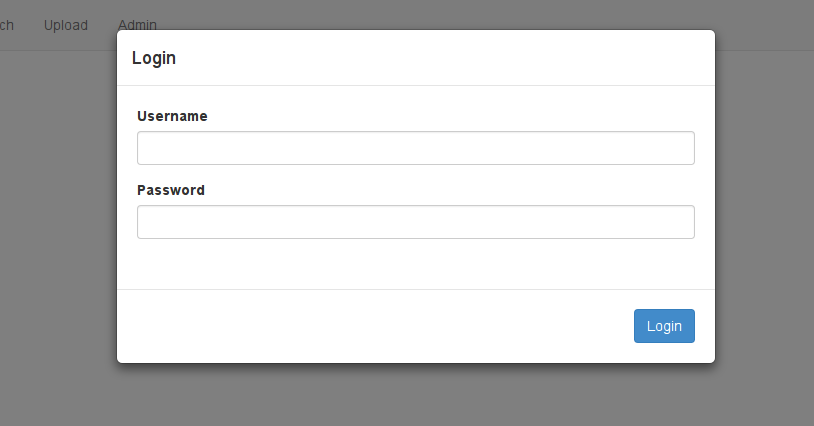
\includegraphics[width=0.75\textwidth]{web/manual/web_login.png}
\caption{\label{fig:web_search_login} The login pop-up window.}
\end{figure}
When first entering the web page, the login pop-up window in \refer{fig:web_search_login} is shown and the user will have to enter their username and password to gain access to the application.

%figure 2
\begin{figure}[h] 
\centering
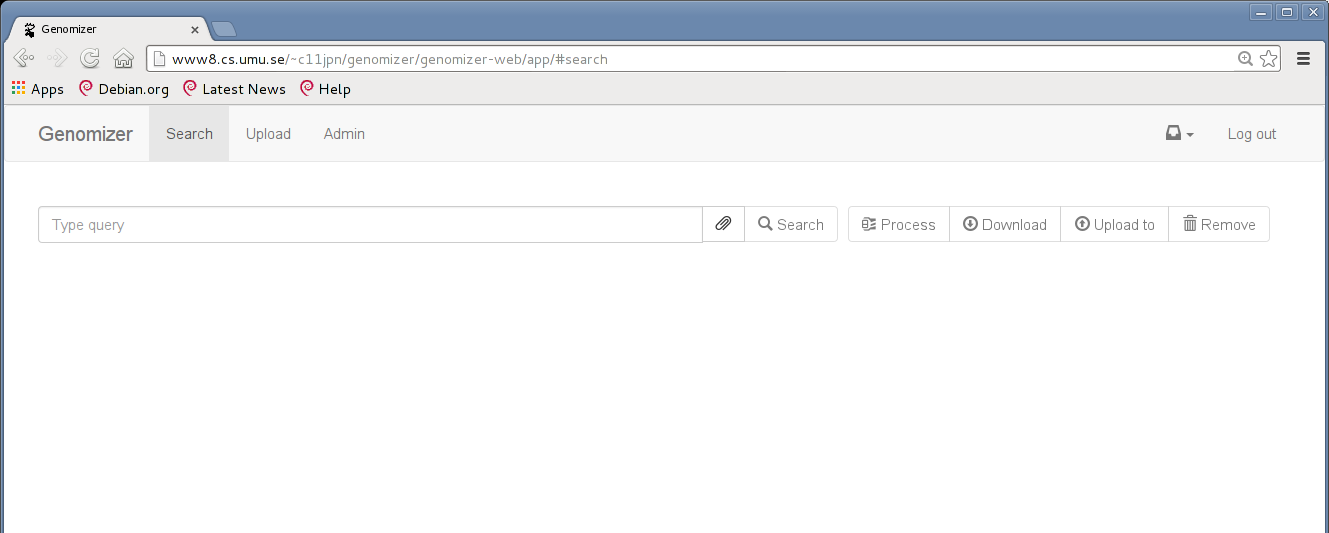
\includegraphics[width=1\textwidth]{web_search_welcome.png}
\caption{\label{fig:web_search_welcome} The start view of the web page.}
\end{figure}

When the user has logged in, the user is taken to the search page as shown in \refer{fig:web_search_welcome}.

The navigation bar at the top has a number of buttons to the left and two buttons to the right with the following functionality:
\begin{itemize}
	\item Clicking the “Genomizer” logo takes the user right back to the start view.
	\item The “Search” button will bring up the search view where the user can enter search strings to be sent to the server, and view search results.
	\item The “Upload” button will bring up the upload view where the user can select files to be uploaded and input annotation to a new experiment.
	\item The “Process” button will bring up the process view where the user can select an experiment to process.
	\item The “Administration” button will bring up the admin view where the user can handle genome releases and annotations.
    \item The inbox icon on the left side opens a dropdown list which displays the statuses of files currently being processed.
    \item The “Log out” button will log out the user.
\end{itemize}
This navigation bar is persistent through all sub pages and can easily be accessed.

\subsubsection{Search view}

In the search view, below the navigation bar, a “search-and-functionality” bar is visible. There is a search field and there are seven buttons that are explained below, starting with the left-most button: 

\begin{itemize}
	\item ”Query builder”, represented by a paperclip, brings up a query builder, shown in \refer{fig:web_search_queryBuilder}, that helps unexperienced users construct a valid query used for searching experiments. Just select a value in the three fields and press add. The correct pubmed-styled query will be shown in the search field and the three query fields will be reset so the user can add more things to search for in their query.
	\item “Search” searches for the query in the search field. 
	\item “Process” processes the selected files. This feature is demonstrated further in \refer{fig:web_process_modalView}.
    \item “Convert” converts the selected files. This feature is demonstrated further in section \ref{sssec:convertView}.
    \item “Upload to” opens the upload view with the selected experiments selected where the user can upload new files to an already existing experiment.
    \item “Remove” opens a new view where the files which are going to be deleted are presented along with a confirmation dialog that the user really wants to delete those files and experiments.
\end{itemize}

\begin{figure}[h]
\centering
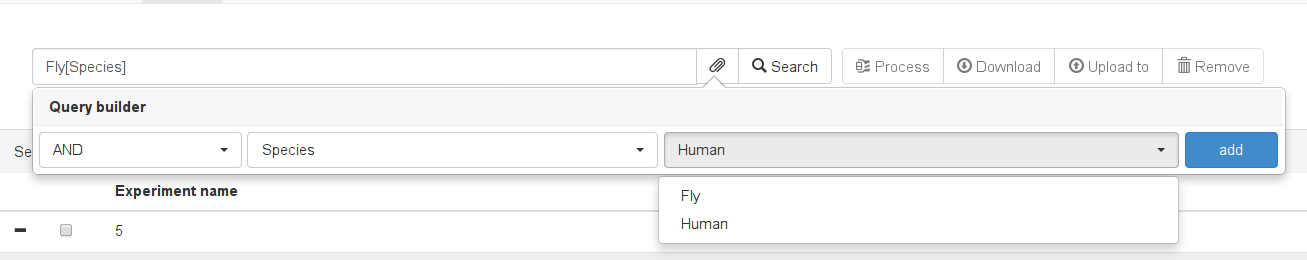
\includegraphics[width=1\textwidth]{web_search_queryBuilder.png}
\caption{\label{fig:web_search_queryBuilder}The query builder.}
\end{figure}

When first entering the search view, only the query builder button and the search button are clickable. The rest of the buttons become clickable once the user selects experiments or files. To search, the user can either write a pubmed style query (for example: \textit{”Fly[Species]”} to search for every experiment with ”Fly” as value of the annotation ”Species”) or use the query builder. When clicking the search button, a loading screen is shown. The experiment data is displayed once it has been retrieved from the server.

%figure x3
\begin{figure}[h]
\centering
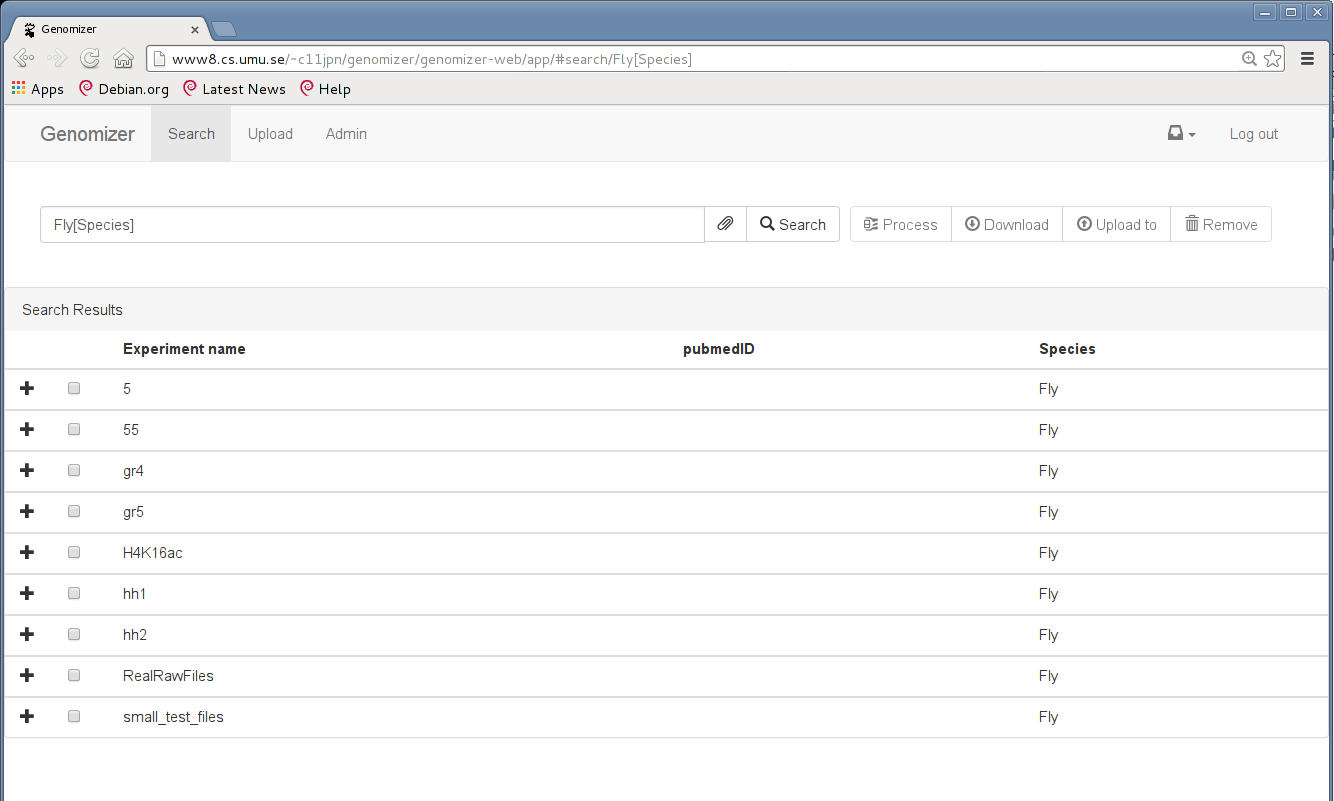
\includegraphics[width=1\textwidth]{web_search_searchTab.png}
\caption{\label{fig:web_search_searchTab}The search tab after searching for \textit{“Fly[Species]”}.}
\end{figure}

The view in \refer{fig:web_search_searchTab} is shown when the user has searched for the query \textit{”Fly[Species]”}. The displayed list contains all experiments returned from the search and a header on top with all annotation types. Every experiment can be expanded by clicking it to show the file types it contains. Each file type can be further expanded to show all files of that type in the experiment. Every file and experiment has a checkbox next to it that is used to select it. In \refer{fig:web_search_searchResult}, an experiment called \class{Ratiotest} and its contained collection of \class{raw} files have been expanded. Furthermore, the files \class{test.fastq} and \class{test2.fastq} have been selected. These files can now, for example, be processed or removed by using the buttons in the “search-and-functionality” bar.

%figure x4
\begin{figure}[h]
\centering
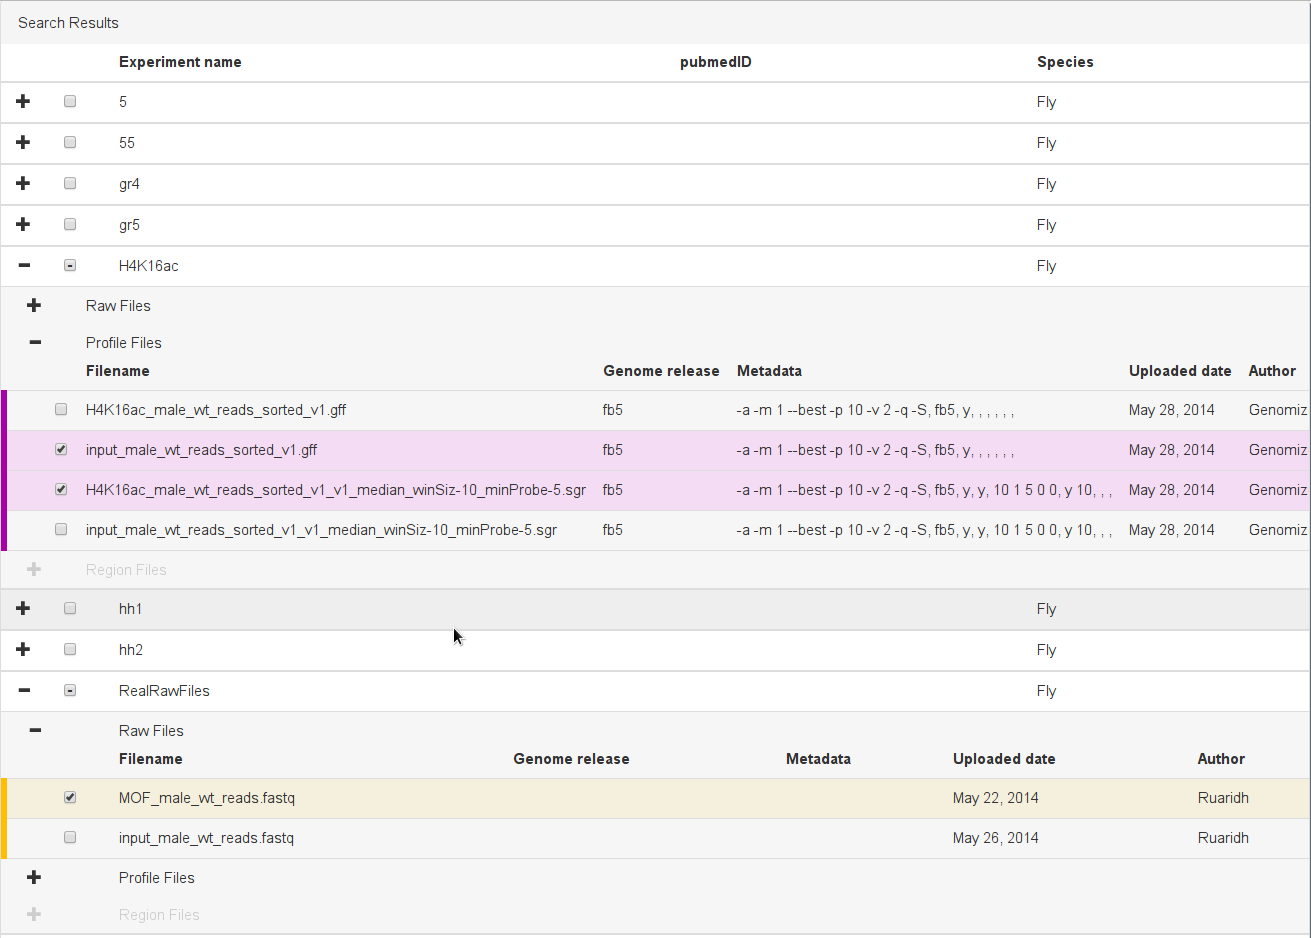
\includegraphics[width=1\textwidth]{web_search_searchResult.png}
\caption{\label{fig:web_search_searchResult}The search results table zoomed in, displaying the information of a \class{raw} file after having expanded an experiment.}
\end{figure}

If no experiments match the search query, the Search Results table will be empty stating “No search results found”.

\pagebreak
\subsubsection{The processing modal}
%figure X6
\begin{figure}[h]
\centering
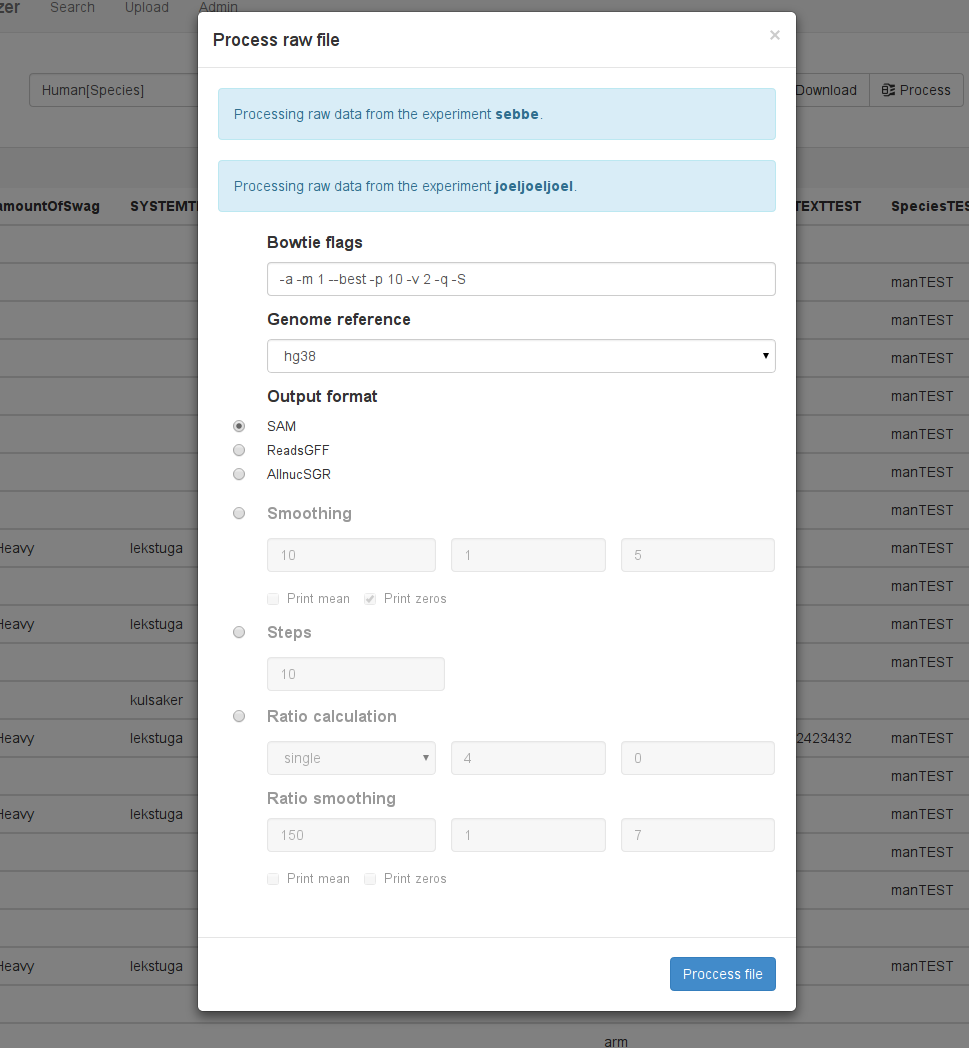
\includegraphics[width=1\textwidth]{web_process_modalView.png}
\caption{\label{fig:web_process_modalView}The processing modal.}
\end{figure}
\FloatBarrier
When the user has selected some files that are going to be processed the user will be presented with the view from \refer{fig:web_process_modalView}. The user can here choose which level of processing should be done on the \class{raw} files.

By clicking the radio buttons on the left side that much processing will be done on the \class{raw} files. All the steps above the selected will also be executed since they are needed to reach that level of processing.
At the top of the modal the experiments currently going through processing are presented.
\begin{figure}[h]
\centering
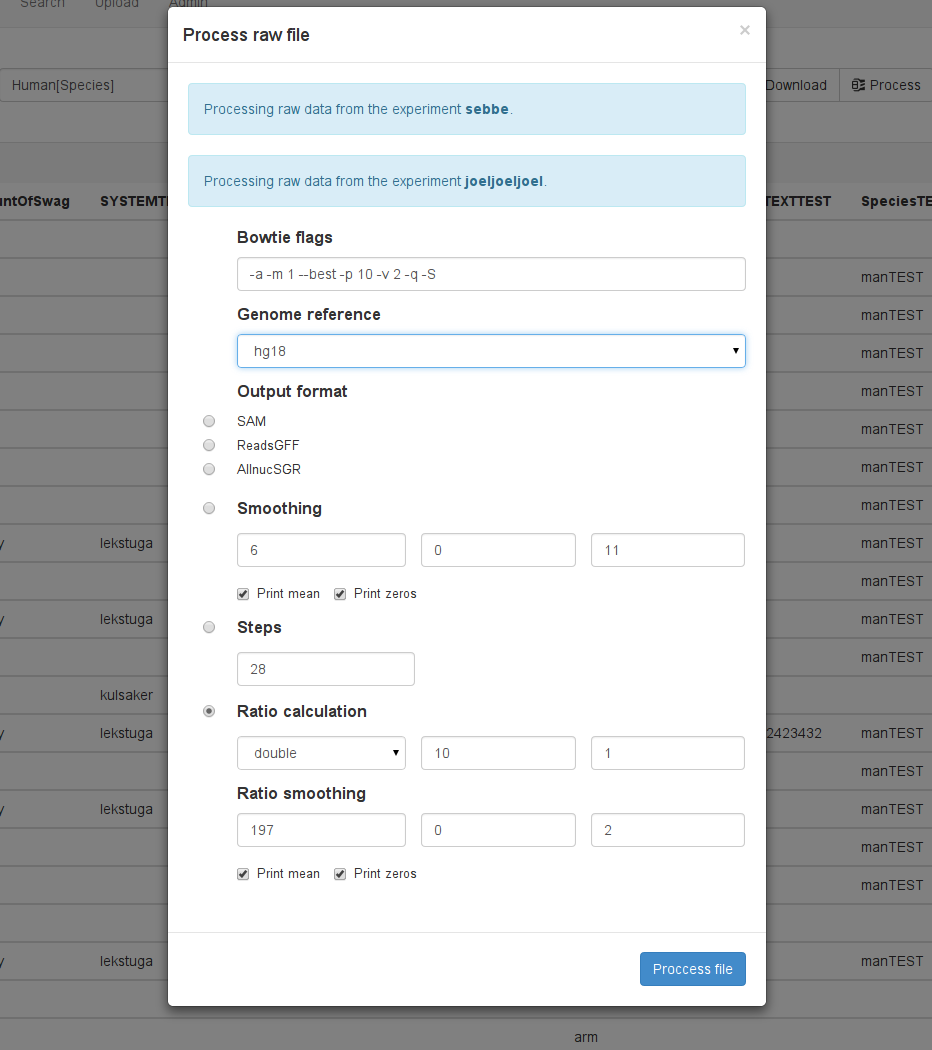
\includegraphics[width=1\textwidth]{web_process_modalValues.png}
\caption{\label{fig:web_process_modalValues}The process modal with selected parameters.}
\end{figure}
\FloatBarrier
When the user has decided the parameters as shown in \refer{fig:web_process_modalValues} and wants to start the processing the process button in the bottom right should be pressed. 
\begin{figure}[h]
\centering
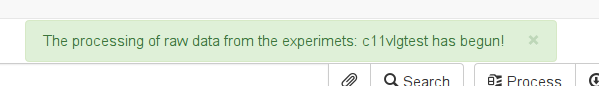
\includegraphics[width=0.8\textwidth]{web_process_success.png}
\caption{\label{fig:web_process_success}Success message.}
\end{figure}
\FloatBarrier
When results are received from the server and they were all successful the processing modal will disappear and a success message indicating that the processing is starting will be displayed to the user like in \refer{fig:web_process_success}.
\begin{figure}[h]
\centering
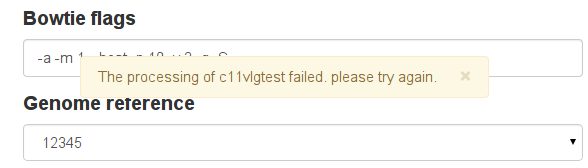
\includegraphics[width=0.8\textwidth]{web_process_notSuccess.png}
\caption{\label{fig:web_process_notSuccess}Fail message.}
\end{figure}
If some of the files that was going to be processed did for some reason fail the user will learn this by a warning message that tells the user which experiment did not start processing and which did as shown in \refer{fig:web_process_notSuccess}. The ones which started to process will be removed from the modal and the ones that did not start to process will remain. The user can now choose other parameters or do something else to make it work and try to submit a processing request again.
\pagebreak



\subsubsection{The convert view} \label{sssec:convertView}

The web application allows conversion between a number of file formats which both are of profile type. More specifically, the user may convert any of the file formats \class{.sgr, .wig, .bed} and \class{.gff} to either \class{.wig} or \class{.sgr}, with the exception that a file cannot be converted to the same file format.

\begin{figure}[h]
\centering
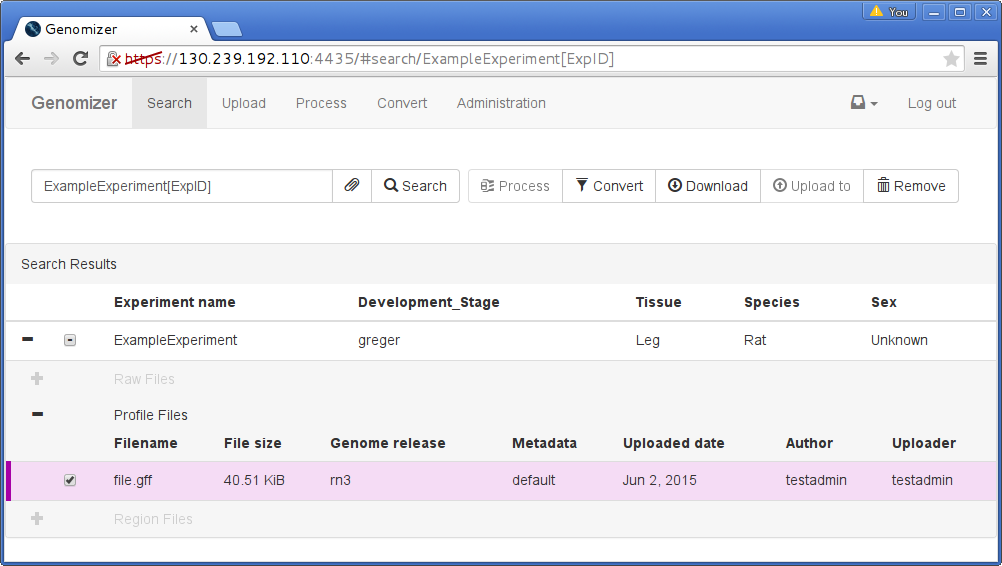
\includegraphics[width=1\textwidth]{web_convert_searchExp.png}
\caption{\label{fig:web_convert_searchExp}Selecting a file to convert.}
\end{figure}

Assume that there is an experiment \class{ExampleExperiment} which contains a profile file \class{file.gff}. Then the experiment will show up in the search view, see \refer{fig:web_convert_searchExp}, when typing ”ExampleExperiment[ExpID]” as search query and then clicking the search button. If the user wants to convert \class{file.gff} to a new file of format \class{.wig} called \class{file.wig}, the following steps can be taken:
\begin{itemize}
	\item From the view in \refer{fig:web_convert_searchExp}, select \class{file.gff} by clicking in its checkbox.
	\item Click the “Convert” button next to the search text field.
	\item The user will now be taken to the convert view shown in \refer{fig:web_convert_convertView}.
	\item Select \class{file.gff} by clicking on it.
	\item Mark the \class{.wig} checkbox in “Convert to” and click the “Convert” button.
\end{itemize}

\begin{figure}[h]
\centering
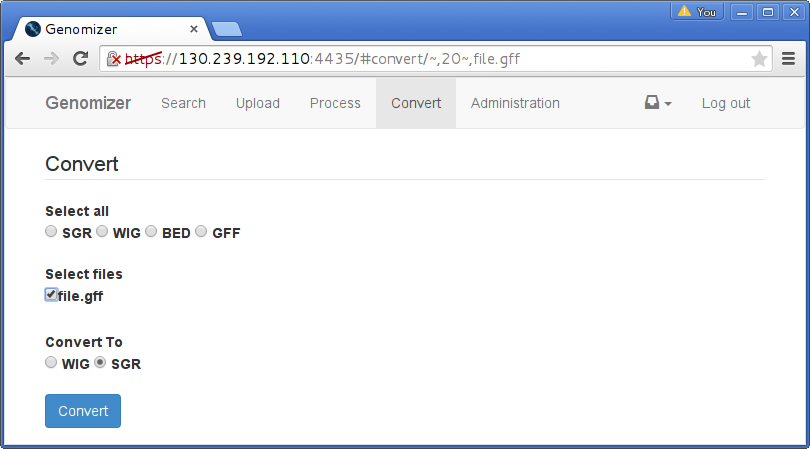
\includegraphics[width=1\textwidth]{web_convert_convertView.png}
\caption{\label{fig:web_convert_convertView}The convert view.}
\end{figure}

The file conversion will now start on the server. Once the conversion is done, the user will be able to see \class{file.wig} listed together with the old file \class{file.gff} when searching for the experiment.

If multiple files are selected for conversion, all of them will appear as a list in the convert view. If the user quickly wants to select all files of a specific file format, for example all \class{.wig} files, the GFF option can be marked in “Select all”. Then all files in the list of the format \class{.wig} will automatically be selected.

\subsubsection{The remove pop-up window}
\begin{figure}[h]
\centering
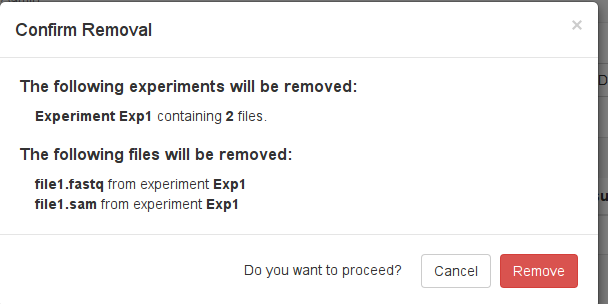
\includegraphics[width=0.8\textwidth]{web/manual/web_remove.png}
\caption{\label{fig:web_remove_removeFiles}The remove pop-up window.}
\end{figure}
\FloatBarrier
When the remove button is pressed the pop-up window in \refer{fig:web_remove_removeFiles} is shown displaying which files and experiments will be removed when the remove button is pressed.


\subsubsection{The process status dropdown}
\begin{figure}[h]
\centering
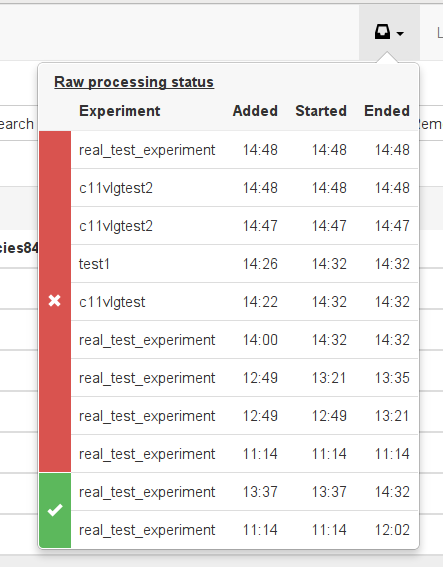
\includegraphics[width=0.5\textwidth]{web_processStatus_withData.png}
\caption{\label{fig:web_processStatus_withData}The process status dropdown.}
\end{figure}
\FloatBarrier
When pressing the inbox icon, a dropdown is shown as in \refer{fig:web_processStatus_withData} displaying the status of experiments currently being processed. There are four different statuses a processing can have, all grouped into colors: Waiting (yellow), Running (blue), Complete (green) and Failed (red). For example, in the figure, the two bottom experiments are complete and the rest have failed. If there are no experiments being processed, the dropdown will simply display “No process status available”.


\subsubsection{The upload view}

%figure X7
\begin{figure}[h]
\centering
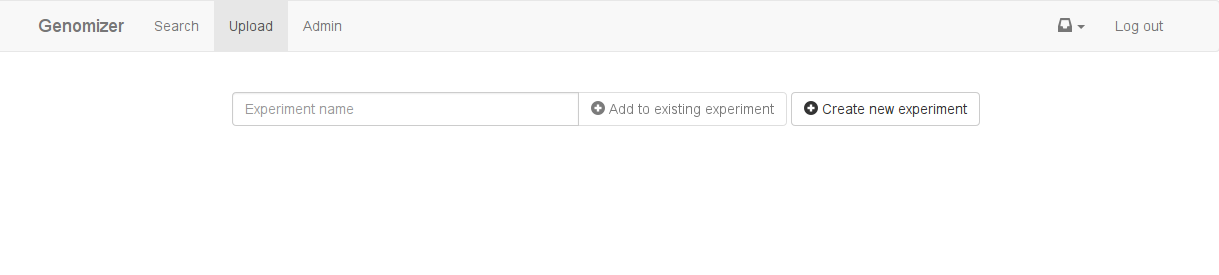
\includegraphics[width=1\textwidth]{web_upload_uploadView.png}
\caption{\label{fig:web_upload_uploadView}The upload view.}
\end{figure}

When the user clicks the upload tab in the navigation bar, the view in \refer{fig:web_upload_uploadView} will appear. The user has the option to create a new and fresh experiment or to load an existing experiment by entering its experiment name. 

%figure X8
\begin{figure}[h]
\centering
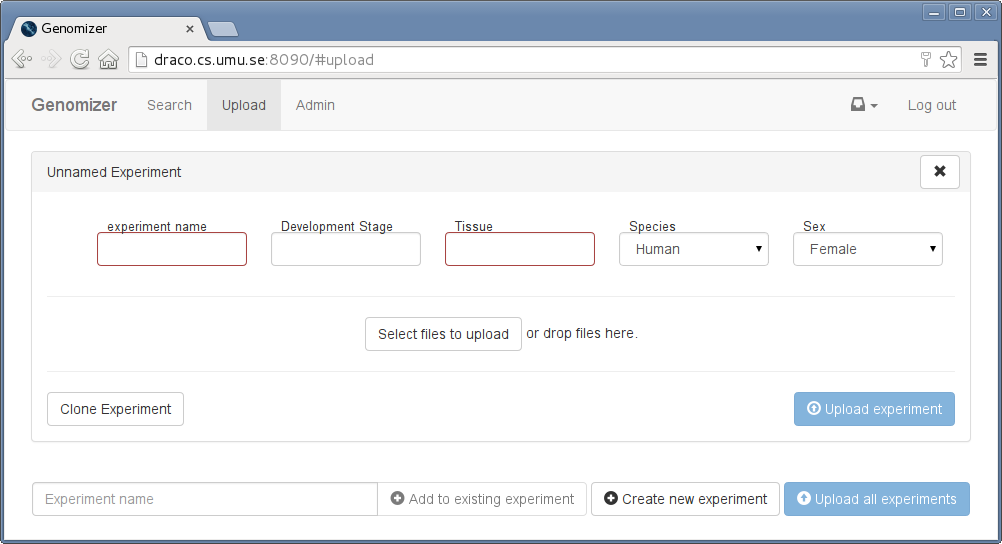
\includegraphics[width=1\textwidth]{web_upload_newExperiment.png}
\caption{\label{fig:web_upload_newExperiment}Creating a new experiment.}
\end{figure}

After clicking the “Create new experiment” button, the view in \refer{fig:web_upload_newExperiment} will appear. Here the user can input the annotations for the experiment through either freetext fields or dropdown lists. If a freetext field has a red border around it, that annotation is required and the experiment cannot be uploaded before all required fields have been filled in and at least one file has been added.

The user can create more experiments by clicking the “Create new experiment” button and a new empty experiment will be placed below the first experiment. The user can also clone an experiment by clicking the “Clone Experiment” button. What happens in this case, is that the every filled-in annotations gets copied to the new experiment.

To add files to the experiments the user can browse for local files and upload them by clicking the “Select files to upload” button. The user will only see file types that have to do with experiments but have the ability to search for all file types. There is also a way of adding files to the experiment by dragging them from a file browser and dropping them onto the experiment “drag and drop”.

An experiment can only contain two \class{raw} files and if the user tries to upload more a message with this information will appear and the experiment cannot be uploaded before the extra \class{raw} file/s is removed. 

To add files to a existing experiment the user types the name of the experiment in the field next to the “Upload to existing experiment” and clicks the button. If the experiment exists on the server it will appear in the experiment view the same way that a new experiment is shown. The annotations of an existing experiment cannot be changed from this view and if there are files already in this experiment they cannot be manipulated. Adding new files to existing experiments works the same way as to a new experiment.

%figure X9
\begin{figure}[h]
\centering
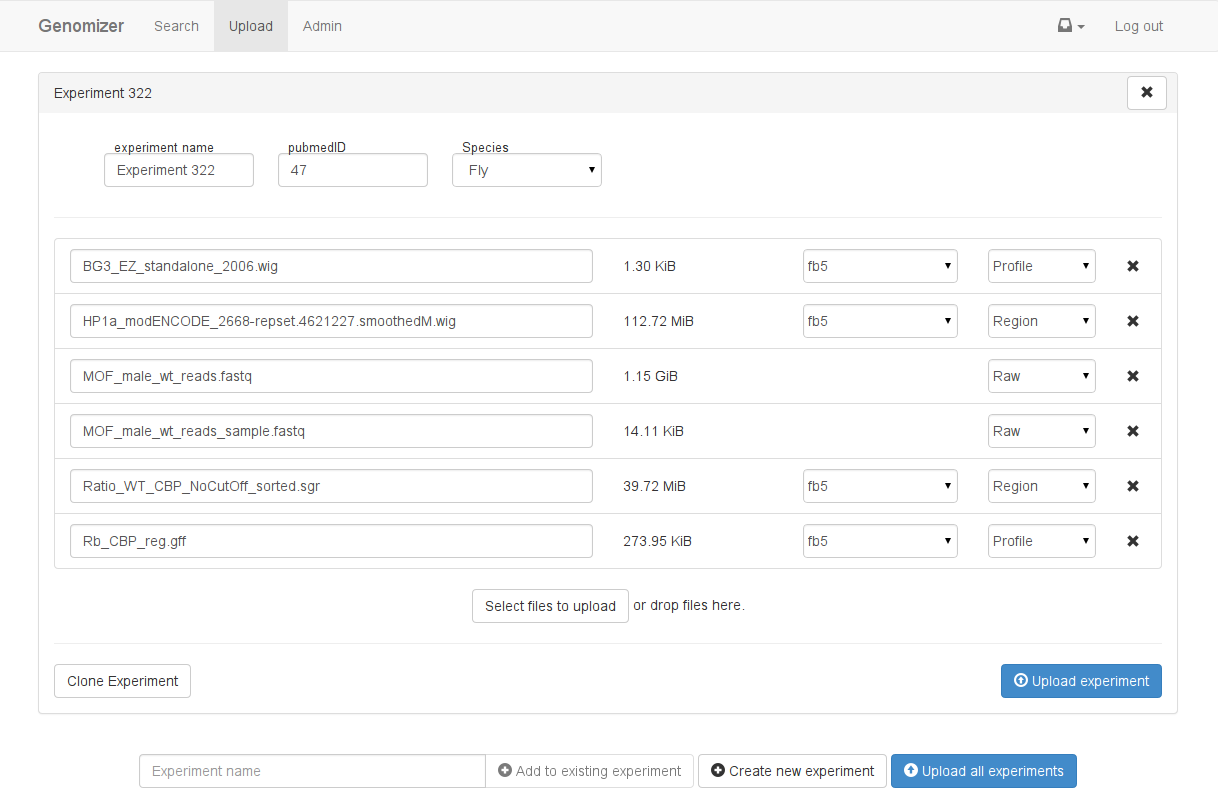
\includegraphics[width=1\textwidth]{web_upload_fileUpload.png}
\caption{\label{fig:web_upload_fileUpload}Files selected for upload.}
\end{figure}
 
When the user selects files, they will appear below the annotations as in \refer{fig:web_upload_fileUpload}. The file name is displayed in a text field on the left side of the file view. Next to the file name is a box that shows the size of the selected file. On the right side there is an option to select what type of file is being uploaded and an option to remove the file from the experiment. If the file type is either \class{profile} or \class{region}, there is an option to select what genome release the file is mapped to. The file type option will automatically be filled in with a guessed value depending on the file ending as follows: \class{.fastq} files are considered \class{raw} and all other formats (\class{.sgr, .wig, .gff}) are interpreted as \class{profile}.

When the user is done selecting files, filling in annotations and clicks the “Upload experiment” button the experiment view will be minimized showing only the name of the experiment and the progress bar of the files being uploaded. When the progress bar is done it turns green and now the experiment with all the files have been uploaded to the server. The user also has a way of uploading several experiments at the same time by clicking “Upload all experiments”. 

\subsubsection{System administration view}

This part of the web application is only accessible if the user has administrator rights. It is integrated with the rest of the web user interface and accessible through the “Administration” tab. The administrator can through this site see all annotations, add new annotations and edit existing ones.

The start page of this section has a “Create New Annotation” button, a list of existing annotations in the database and an edit button per existing annotation. The view looks like in \refer{adm__web_annotationView}. 

\begin{figure}[h]
 \addImage{web_SysadminAnnotationView.jpg}
 \caption{The start page for the administrator in the web client.}
 \label{adm__web_annotationView}
\end{figure}

For each annotation in the annotations list, an “Edit” button is available. When pressed, it will take the user to a page in which they can edit the selected annotation to change its name and what values the dropdown list will have if it is not a freetext field (see \refer{adm_web_editView}). 

\begin{figure}[h]
 \addImage{web_SysadminEditView.jpg}
 \caption{The edit annotation view.}
 \label{adm_web_editView}
\end{figure}
In the edit page, the admin can see the attributes of the chosen annotation and is able to delete the chosen annotation or change the information of it. The “Delete Annotation” button will delete the whole annotation, and for that reason two pop-up windows will appear to confirm that the administrator is sure of the action.

The administrator can change the list of annotation values. The site will automatically check whether something is added, removed or both and sends a request to change the annotation values to the server when the “Update Annotation” button is clicked.

If the admin clicks on the “Create new annotation” button from the admin start page, another view will open with the following structure:
\begin{itemize}
 \item Annotation Name
 \subitem Admin can enter a name for the annotation.
 
 \item Annotation Types
 \subitem Yes/No/Unknown - creates a dropdown list with those three options.
 \subitem freetext - creates an annotation where the users will be able to enter anything.
 \subitem Dropdown list - will enable a fourth field enabling the admin to enter which items that this list will contain.
 
 \item Forced Annotation
 \subitem Admin can choose if the new annotation should be required by users to enter. 
\end{itemize}

A Create Annotation will, if all necessary information has been entered, result in a popup (see \refer{adm_web_createPopup}) showing the resulting annotation and if confirmed, the annotation is added to the database. 
If canceled the administrator can keep making changes or go back to exit this view. If not all values is entered the admin will be alerted of the mistake and nothing will be created.

\begin{figure}[h]
 \centering
 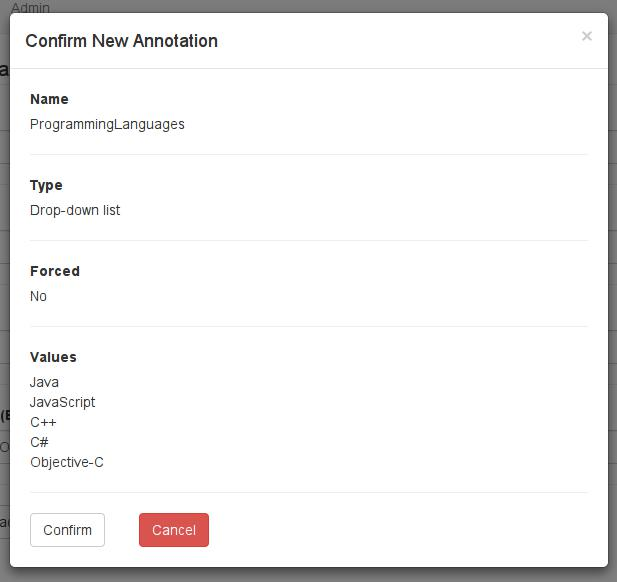
\includegraphics[width=0.7\textwidth]{web_SysadminCreateAnnotationConfirm.jpg}
 \caption{The confirm annotation pop-up.}
 \label{adm_web_createPopup}
\end{figure}



The example in \refer{adm_web_createPopup} will result in a drop-down annotation with the name Number of toes and possible values: 0, 1, 2, 3, 4, 5 with 0 as default and is not forced.

A back button which takes the user back to the annotations start page is also available in this view. In \refer{adm_web_createView} the create annotation view can be seen.

\begin{figure}[t]
 \addImage{web_SysadminCreateAnnotation.jpg}
 \caption{The view for administrators where new annotations can be created.}
 \label{adm_web_createView}
\end{figure}

The “Genome-releases” link on the sidebar takes the administrator to a page where it is possible to add and remove genome releases to and from the server (see \refer{adm_web_genomereleaseView}.

\begin{figure}[h]
 \addImage{web_SysadminGenomeReleaseView.jpg}
 \caption{The genome-release view.}
 \label{adm_web_genomereleaseView}
\end{figure}

The button “Select files to upload” opens the native file explorer where the user can select one ore multiple files and click on “OK”. This will open a popup-window, seen in \refer{adm_web_uploadconfirm}, showing what files that where chosen and asks for species and genome version before uploading. 

\begin{figure}[h]
 \centering
 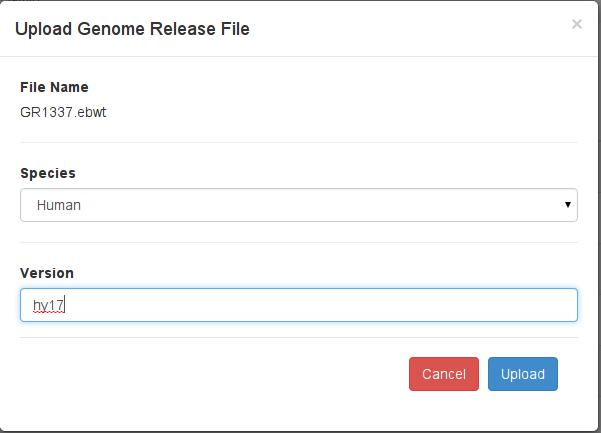
\includegraphics[width=0.7\textwidth]{web_SysadminUploadGenomeReleaseModal.jpg}
 \caption{Popup for uploading genome releases.}
 \label{adm_web_uploadconfirm}
\end{figure}

When the upload begins the popup closes and a progress-bar appears showing the progress, showing ''Upload completed'' when done. The user can at this stage move between pages without disturbing the upload but should not close or refresh the web browser. 

Every genome release in the table can be deleted by clicking on the “Delete” button next to the release. This will prompt a small popup asking for user confirmation and if given a positive response, deletes the genome release from the server and updates the view. 

If any genome release is used by an experiment already an error will appear telling the user exactly that. 

\subsection{Setting up the application}
To setup the application, move the content of the folder \url{genomizer-web/app/} to the desired location from where the application should be run. To run the web page, open a web browser and enter the url to the folder which contains the \class{index.html} file (where the content of app was placed).
For example, given that the \url{genomizer-web} folder is placed in the home folder of the Umeå university CS user \class{c12abc} and that user wants to put the web app in a folder called \url{public/html/} which is also in the home folder of the user. In Linux, do the following steps:
\begin{enumerate}
	\item Navigate to the app folder: \texttt{“cd ~/genomizer-web/app/”}
	\item Move the contents of app to the folder \url{public/html}: \texttt{“mv * ~/public\_html/”}
	\item Given that the url to \url{public/html} is: \filePath{“www8.cs.umu.se/~c12abc/”}
	\item To run the application start a web browser and type \filePath{“www8.cs.umu.se/~c12abc/”}
\end{enumerate}
This will open the web page in the browser.


\FloatBarrier

\section{Android application}
In this section instructions for the usage of the \appName\ Android application is presented. In \refer{sec:and_start} there is a description on how to start the application and \refer{sec:and_search} gives instructions on how to search for experiments.

\subsection{Start the Application and Login}
\label{sec:and_start}

%Localize the \appName\ icon in your list of Android applications and click the icon in order to start \appName.

The user needs to login in order to start working with the \appName\ app. The  user name and password is inserted in the corresponding boxes and the clicking the \term{Sign in} button initiates the main application. If you dont have a user name or password, the system administrator should be contacted to help with the creation of an account.

\begin{figure}[h]
\addScaledImage{0.1}{figures/and_login.png}
\caption{Login View}
\label{fig:and_login_man}
\end{figure}
\FloatBarrier


In \refer{fig:and_login_man}, the tool button in the upper right corner leads to the \term{Settings View}, described in  \refer{sec:and_manual_settings} below.

\subsection{Settings}\label{sec:and_manual_settings}
The \term{Settings} view acts to enable the user to choose which server to connect to when using the Genomizer application. As of the current release of the application, in the Settings View, the user is able to:

\begin{enumerate}
\item Select one of previously used server URLs
\item Add a server URL
\item Remove a server URL
\item Edit an existing server URL
\end{enumerate}

The left most image in \refer{fig:and_settings_man} show three buttons in the top right corner of the view. These buttons are used to access the functionalities listed above. The button with a green plus sign enables the user to add a new server URL, as illustrated in the image in the middle of \refer{fig:and_settings_man}. The button in the middle with a paint brush icon will on selection show the server URL edit view, as illustrated in the right most image in \refer{fig:and_settings_man}. And the left most button with a red cross icon will upon selection enable the user to remove the currently selected server URL from the drop down menu containing all saved server URLs.


Any selection, removal, edit or addition of server URLs are stored locally on the device and and are loaded upon subsequent application launches.


\begin{figure}[h]
\addThreeImages
{figures/and_server_settings_select.png}
{figures/and_server_settings_add.png}
{figures/and_server_settings_edit.png}
\caption{Settings View}
\label{fig:and_settings_man}
\end{figure}
\FloatBarrier


\subsection{Searching for files}\label{sec:and_search}

When entering the Search View, as illustrated in \refer{fig:and_search_man} all annotations are automatically downloaded from the server and displayed as a list. Each annotation consists of an annotation-identifier, a dropdown table/text-input field where the user may specify desired value, and a checkbox. When putting a check-mark in the checkbox, it means that this particular annotation type should be used when searching for files in the database. The search is initiated by pressing \term{Search} at the bottom of the view.

Once the user has been logged in to the system, three buttons will always be visible in the top right corner of each view:
\begin{enumerate}
\item Search button
\item Selected Files button
\item Process Status button
\end{enumerate}

Clicking these buttons switches the context of the application and allow the user to quickly navigate between different functionalities.

The search view also contain a button visible in the top right corner, used to activate the advanced search mode described in the following \refer{sec:and_search_pub}. 

\begin{figure}[h]
\addScaledImage{0.1}{figures/and_search.png}
\caption{The Search View}
\label{fig:and_search_man}
\end{figure}
\FloatBarrier


\subsection{Pubmed Search}\label{sec:and_search_pub}
The Pubmed Search view provide the means of free-text search using Pubmed-Style queries as seen in \refer{fig:and_pubmed_man}. This view include a text-input field together with two buttons. The text field  is populated with the annotations that the user may have selected within the regular Sarch View. However, if no annotations have been previously selected in the Search View, the user must input all annotations manually. The annotations selected in the Search View are associated with logical connectives. These logical connectives, as well as annotation values, can be manually modified by the user. The supported logical connectives are: 

\begin{enumerate}
\item AND
\item NOT
\item OR
\end{enumerate}

The user may also choose to provide perentheses to device more specific searches.

\begin{figure}[h]
\addScaledImage{0.1}{figures/and_search_advanced.png}
\caption{The Pubmed Search View}
\label{fig:and_pubmed_man} 
\end{figure}
\FloatBarrier


%Explains several steps, remove others or shorten this?
\subsection{Search Results}
When searching the user will be redirected to the search results view  that displays a list of available experiments matching the search annotations. Every experiment is listed showing the experiment name. To receive more information about data files that are available for each experiment, click on an experiment in the list. By clicking an entry you will be taken to a new view displaying all available data files for that experiment, presented in the Experiment List View. 

Clicking on the cogwheel button in the top right corner of the view enables the user to modify which annotations are presented within the Search Results View, and is described further in the following \refer{sec:search_settings}.

\begin{figure}[h]
\addScaledImage{0.1}{figures/and_search_result.png}
\caption{The Search Results View}
\label{fig:and_search_results_man} 
\end{figure}
\FloatBarrier


\subsection{Search Settings View}\label{sec:search_settings}
The Search Settings View display settings for the files presented to the user after a search is done, as illustrated in  \refer{fig:and_search_settings_man} below. The Search Settings View contains all different annotations the user will be able to display about the experiments presented in the Search Results View. The user are able to select annotations by marking the checkbox next to the annotation name and then clicking the Save settings button to save changes. If the user has no special requests it is also possible to use default settings, which will display (experiment-Id, created by, pubmed and type) annotations for the files displayed. 



\begin{figure}[ht]
\addScaledImage{0.1}{figures/and_search_select_visible_annotations.png} 
\caption{Search Settings View}
\label{fig:and_search_settings_man}
\end{figure}
\FloatBarrier


\subsection{Experiment File View}
The Experiment File View is used to present the user with all files associated with an experiment. This includes all raw, profile and region files derived from the experiment. A user may select and add an arbitrary number of files to the Selected Files view, which is described in \refer{sec:and_manual_selected}, by marking the checkbox of the desired files, as done in  \refer{fig:and_experiment_man}, and pressing \term{Add to selection}.

Clicking on a file presented within this view creates a popup containing all different annotations for the selected file, as illustrated in the right most image in \refer{fig:and_experiment_man}.

\begin{figure}[h]
\addTwoImages{figures/and_experiment_files.png}{figures/and_experiment_file_info.png}
\caption{The Experiment File View}
\label{fig:and_experiment_man}
\end{figure}
\FloatBarrier






\subsection{Selected Files}\label{sec:and_manual_selected}
Once the user has signed in to the server, the user is presented with a \term{Selected Files} view, as illustrated in \refer{fig:and_selected_man}.
This is the main part of the application where all work and conversions are done to files, when the user has searched and found files that are interesting for further use, it can be moved to the selected files area. 
The page contains three different tabs that the user may use to show different type of files saved in the selected files workarea. All files stored in this page are only saved during the current session and is meant to be used as a temporary grouping area for files. 

\begin{itemize}

	\item \term{Raw}, will diplay all the Raw files that the user has choosen to save to the temporary work area. The files here can be marked and used for converting to profile data.
    \item \term{Profile}, will display the Profile files that the user has choosen to move to the selected files area. No conversions or other work can be done at this stage to profile files.
    \item \term{Region}, this page will display all the region files the user has selected to move to the selected files area for further work. No conversions or other work can in this stage be done to region files.
    
\end{itemize}

Similar to the Experiment View, clicking on a file will present the user with a popup containing the annotations for that file.


\begin{figure}[h]
\addTwoImages{figures/and_selected_files.png}{figures/and_selected_files_file_info.png}
\caption{Selected Files View}
\label{fig:and_selected_man}
\end{figure}
\FloatBarrier


\subsection{Converting Files}
When the user has choosen a file (or several files) for conversion, the user will be presented with the Conversion View as seen in \refer{fig:and_conversion_man}. In this view the user may enter the parameters needed to perform a Raw-to-Profile-file conversion.
\newline
There are 9 different parameters to be specified in this page for the conversion to be done in a proper way. All parameters do not have to be filled, but they have to be specified in the order that is presented to the user. In order to fill out parameter number 3, both parameter 1 and 2 have to be filled out first.

\begin{enumerate}
	\item \term{Bowtie}, is a freetext field where the different parameters for the bowtie program are to be inserted.
    \item \term{Genome Version}, is a dropdown menu where the user is presented with all the different genome versions that can be used for the conversion.
    \item \term{Sam to GFF}, is an on/off option.
    \item \term{GFF to SGR}, is an on/off option. 
    \item \term{Smoothing}, free text field for the parameters for smoothing if it is to be used.
    \item \term{Stepsize}, free text field for which stepsize is to be used for the conversion.
    \item \term{Ratio calculation}, on/off field which determines if the ratio calculation is to be used. If checked it will require both next two fields to be filled out.
    \item \term{Ratio}, free text field with the parameters for the ratio, if ratio calculation is wanted.
    \item \term{Smoothing}, free text field for parameters regarding the smoothing for the ratio calculation.     

\end{enumerate}

\begin{figure}[h]
\addScaledImage{0.1}{figures/and_convert_view.png}
\caption{The Conversion View}
\label{fig:and_conversion_man}
\end{figure}

\FloatBarrier


\subsection{Process View}
The process view, as illustrated in \refer{fig:and_process_man} below, is used to visualize the current workload on the server. The view contains a list of tasks that has been assigned to the server. Each task contains the name of the experiment in which the process is currently operating in, the time when the process was added, the time when the process was started and the time when the process was finished. Each item also contains information about the process current state.

Each process may have one of these four states:
\begin{enumerate}
\item{Waiting} - The task is awaiting processing by the server
\item{Started} - The task is currently being processed by the server
\item{Finished} - The task has been completed
\item{Crashed} - The task was not successfully completed
\end{enumerate}

\begin{figure}[h]
\addScaledImage{0.1}{figures/and_process_status.png}
\caption{ The Process View}
\label{fig:and_process_man}
\end{figure}

\FloatBarrier


\FloatBarrier

\section{iOS application}
\subsection{How to run the app in Xcode}
In order to use the program, import the project from github into Xcode from the following repository:
\url{https://github.com/genomizer/genomizer-iOS.git} 

To compile and run the program, press \click{cmd+R}. A simulator will start and the login screen will be shown as seen in \refer{fig:ios_login}a.

\subsection{How to login}

\begin{enumerate}
\item Tap the settings button in the upper right corner and enter the url and port for the server you want to use and press \click{Done}. See \refer{fig:ios_login}a,c.
\item Tap on the \click{Username} textfield and enter your username.
\item Tap on the \click{Password} textfield and enter your password.
\item Tap on \click{Sign in} to sign in.
\end{enumerate}
A user gets logged in when accepted credentials are entered in the ‘username’ and ‘password’ fields and the ‘Sign in’ button is pressed. If incorrect credentials are entered, a popup message is shown, informing the user that the username or password is incorrect.

\begin{figure}[ht]
\addThreeImages{ios_login1.PNG}{a}{ios_login2.PNG}{b}{ios_login3.PNG}{c}
\caption{The login screen.}
\label{fig:ios_login}
\end{figure}
\FloatBarrier

\subsection{How to logout}
\begin{enumerate}
\item Tap \click{Gear}-symbol on the tab bar and a \emph{Setting}-screen will appear. See \refer{fig:ios_more}
\item Tap \click{Logout} to logout.
\end{enumerate}

\begin{figure}[htb]
\addScaledImage{0.17}{ios_settings.PNG}
\caption{The settings screen.}
\label{fig:ios_more}
\end{figure}
\FloatBarrier

\subsection{How to search for experiments}

\begin{enumerate}
\item Ensure that you on the search-screen by looking at the title on the top. If it says \emph{Search} you can skip step (2). 
\item Tap on leftmost button(magnifying glass) on the tab bar which you can find on the bottom of the screen.
\item Tap on the annotation you want to search for and a spinning wheel with options will appear from the bottom of the screen. See \refer{fig:ios_search}a.
\item Drag the wheel up or down to select the option you want.
\item Enable the annotation to use when searching by toggling the switch to the right of the annotation. See \refer{fig:ios_search}b.
\item Do steps (2)-(4) for more search criteria.
\item Tap \click{Search} to search.
\end{enumerate}

\begin{figure}[ht]
\addThreeImages{ios_search1.PNG}{a}{ios_search2.PNG}{b}{ios_search4.PNG}{c}
\caption{The search screen.}
\label{fig:ios_search}
\end{figure}
\FloatBarrier

\subsection{How to use advanced search}

\begin{enumerate}
\item Ensure that you on the search-screen by looking at the title on the top. If it says \emph{Search} you can skip step (2). 
\item Tap on leftmost button(magnifying glass) on the tab bar which you can find on the bottom of the screen.
\item Tap on the symbol to top right of the screen and a new view will appear with the title \emph{Advanced Search}. See \refer{fig:ios_search}c.
\item Write your search criteria in PubMed-style and tap \click{search}
\end{enumerate}
The annotations you select on the search-screen will also show in advanced search.

\subsection{How to process files}


\begin{enumerate}
\item Search for experiments
\item In \emph{Search Results}-screen tap on an experiment and the \emph{Files}-screen will appear showing the files which belongs to the experiment. See \refer{fig:ios_files_view}a
\item Tap the \click{Plus}-symbol next to the file you want to process.
\item Do step (3) for every file you want to process. Same file can be used more than once. A counter will appear next to the Plus-symbol to keep track on how many times the file will be used in the process-step, see \refer{fig:ios_files_view}b.
\item Tap the \click{Process}-button and \emph{Make a process}-view will appear with every file you have selected. See \refer{fig:ios_make_process_view}a
\item Tap \click{Add Process} and select what kind of process you want to do on the selected files.
\item After you have selected a process the input files and output files will appear with the selected process separating them. You can add parameter values by tapping \click{Flag}-symbol below the input files. The output files can be renamed by tapping on the filename. See \refer{fig:ios_make_process_view}b
\item Do step (6) to create a sequence of processes to be made on the selected files. See \refer{fig:ios_make_process_view}c for an example of a process sequence.

\item Tap \click{Done}-button to send the sequence of processes to the server.
\end{enumerate}

%\begin{figure}[htb]
%\addScaledImage{0.17}{ios_process_files.jpg}
%\caption{Files screen.}
%\label{fig:ios_process_files}
%\end{figure}
%\FloatBarrier

\begin{figure}[htb]
\addTwoImages{ios_process_files.jpg}{a}{ios_files_added.jpg}{b}
\caption{Files view.}
\label{fig:ios_files_view}
\end{figure}
\FloatBarrier

\begin{figure}[htb]
\addThreeImages{ios_empty_make_process.jpg}{a}{ios_one_process.jpg}{b}{ios_many_process.jpg}{c}
\caption{Create processes.}
\label{fig:ios_make_process_view}
\end{figure}
\FloatBarrier


\subsection{How to set which annotation to be visible on Search Results}

\begin{enumerate}
\item In Search Results view, tap \click{Edit} and \emph{Select Annotations}-screen will appear
\item Select which annotations to show by toggle the switch next to each annotation.
\item Tap \click{Back} to go back to \emph{Search Results}. See \refer{fig:ios_searchResult}a-c
\end{enumerate}

\begin{figure}[ht]
\addThreeImages{ios_result1.PNG}{a}{ios_result2.PNG}{b}{ios_result3.PNG}{c}
\caption{Select annotation}
\label{fig:ios_searchResult}
\end{figure}
\FloatBarrier

%\subsection{How to remove files from workspace}
%\begin{enumerate}
%\item Tap \click{Star}-symbol on the tab bar to view the workspace.
%\item Toggle the switch next to the file you want to remove.
%\item Tap \click{Trash can}-symbol to the upper right corner to remove the selected files. See \refer{fig:ios_selectedFiles}
%\end{enumerate}

\subsection{How to view process status on the server}

\begin{enumerate}
\item Tap \click{Process}-symbol(the symbol between the star and the trash can) to view the processes on the server.
\item To refresh the view, drag the view down until an activity indicator icon is visible below the title of the screen and release. See \refer{fig:ios_processes}
\end{enumerate}

\begin{figure}[htb]
\addScaledImage{0.3}{ios_processes1.PNG}
\caption{The select task screen.}
\label{fig:ios_processes}
\end{figure}
\FloatBarrier

\subsection{How to view information about a file}

\begin{enumerate}
\item Tap \click{information}-symbol next to the file to view information of the file.
\item Close by tapping \click{Close}. See \refer{fig:ios_files1}a-b
\end{enumerate}

\begin{figure}[htb]
\addTwoImages{ios_files4.PNG}{a}{ios_files2.PNG}{b}
\caption{The files screen.}
\label{fig:ios_files1}
\end{figure}
\FloatBarrier




\FloatBarrier


\chapter{Deployment and maintenance}
%This section describes how administrators and developers can deploy and maintain the system. Directed towards administrators. Start with subsection here.

This chapter is directed towards administrators and developers that wants to set up a server and install the software needed to get a fully functional system. It also gives instructions on how to maintain the system in case of problems that can arise.

\section{Configure server}
This chapter is directed towards administrators and developers who want to
set up a server and install the software needed to get a fully functional system.
It also contains instructions on how to maintain the system in case problems arise.
\section{Manuals}
To set up the server with the necessary software and configurations two guides are available. These two manuals are created to help a system administrator in the installation process of the server machine needed for the project. The manuals are written for configuration of the server on two different operating systems, Ubuntu 14.04 and Debian 7.5. 

The manuals can be found in Appendix \ref{chap:exp_app_ubuntu} and \ref{chap:exp_app_debian}.

\section{Configuration}
The \appName\ system needs special configuration to work properly. See the manual for the running operating system to get the correct settings for the \appName\ server machine. All settings can be changed, but when changed the system may not work properly anymore. Please only make changes that are documented in the corresponding manual.


\section{Administer the database}
This chapter contains instructions for setting up the postgresql database and user accounts.

    \subsection{Set up postgresql account}
      This step is only required if you do not already have a \texttt{psql} username and password. If you have been assigned this from a sysadmin proceed to \emph{Upload SQL Script to server}.

    \begin{enumerate}
      \item Log in to the server:
      \begin{verbatim}
> ssh <username>@<host>
      \end{verbatim}

      \item Become sudo-user “postgres”:
      \begin{verbatim}
> sudo su postgres
      \end{verbatim}

      \item Add yourself as a postgresql user:
      \begin{verbatim}
> createuser <username>
      \end{verbatim}

      \item Log into postgresql as root:
      \begin{verbatim}
> psql
      \end{verbatim}

      \item Set your password:
      \begin{verbatim}
> \password <username>
      \end{verbatim}

      \item Create database:
      \begin{verbatim}
> create database genomizer;
      \end{verbatim}

      \item Grant yourself all permissions on the \appName\ database: \begin{verbatim}
> grant all on database genomizer to <username>;
> \q
      \end{verbatim}

      \item Navigate to postgresql configuration folder:
      \begin{verbatim}
> cd /
> cd etc/postgresql/9.3/main
      \end{verbatim}

      \item Navigate to postgresql configuration folder:
      \begin{verbatim}
> sudo nano postgresql.conf
      \end{verbatim}

      \item Change connection settings:\\Locate line: 
      \begin{verbatim}
#listen_adresses = ‘<settings>’    # what IP address(es) to listen on;
      \end{verbatim}
      Change to:
      \begin{verbatim}
listen_addresses = '*'    # what IP address(es) to listen on;
      \end{verbatim}

      \item Write changes and exit:\\
      Hold down ctrl and press o\\
      Hold down ctrl and press x

      \item Open configuration file:
      \begin{verbatim}
> sudo nano pg_hba.conf
      \end{verbatim}

      \item Change Client Authentication Configuration:\\Locate the heading: 
      \begin{verbatim}
# IPv4 local connections:
      \end{verbatim}
      Under the heading, add the line:
      \begin{verbatim}
host    all    all    127.0.0.1/32    md5
      \end{verbatim}

      \item Write changes and exit:\\
      Hold down ctrl and press o\\
      Hold down ctrl and press x

      \item Restart postgresql:
      \begin{verbatim}
> cd /
> sudo /etc/init.d/postgresql restart
      \end{verbatim}

    \end{enumerate}

    \subsection{Upload SQL Script to server}

    \begin{enumerate}

      \item In a termainal window navigate to the folder where the \verb+genomizer_database_tables.sql+ script resides.

      \item Establish secure ftp connection to the server:
      \begin{verbatim}
> sftp <username>@<host>
      \end{verbatim}

      \item Create a new folder on the server:
      \begin{verbatim}
> mkdir SqlScripts
      \end{verbatim}

      \item Upload \verb+genomizer_database_tables.sql+:
      \begin{verbatim}
> put genomizer_database_tables.sql SqlScripts/
      \end{verbatim}

      \item Exit \texttt{sftp}:
      \begin{verbatim}
> exit
      \end{verbatim}

    \end{enumerate}

    \subsection{Create the \appName\ Tables}

    \begin{enumerate}

      \item Log in to the server:
      \begin{verbatim}
> ssh <username>@<host>
      \end{verbatim}

      \item Log in to the database:
      \begin{verbatim}
> psql genomizer
      \end{verbatim}

      \item Run \verb+genomizer_database_tables.sql+
      \begin{verbatim}
> \i SqlScripts/genomizer_database_tables.sql
      \end{verbatim}


    \end{enumerate}

The \appName\ database is now ready to use.


\section{Install the server}
To start the server, java needs to be installed on the computer and a runnable JAR file needs to be created.
There are many ways to create such a file, for example, the terminal or
an IDE like eclipse could be used. \\The server also needs a database to work properly. This guide assumes that a database is present, otherwise a new database needs to be created and currently hardcoded into the server.\\
\\
The creation of the runnable JAR file in the IDE eclipse will be explained in \ref{sec:com_UsingEclipse} below.
\subsection{Using eclipse to create a runnable JAR file}
\label{sec:com_UsingEclipse}
This guide was written 2014-05-09 which means that the process of creating the runnable JAR file with eclipse might have changed slightly, but the main idea should still be valid.\\
\\
To create the runnable JAR file with eclipse, follow these steps:
\begin{enumerate}
\item Open eclipse and import all the code into a project.
\item Rightclick on the project and choose export.
\item Expand the folder "java" and then choose "runnable JAR file".
\item Make or choose an already existing launch configuration where ServeMain is the class containing the main-method.
\item Choose an export location for the runnable JAR file.
\end{enumerate}

\subsection{Starting the server}
Here the actual startup of the server will be explained in a step by step manner.
In order for this to work, the runnable JAR file must have been created.
\begin{enumerate}
\item Choose a computer that should host the server.
\item Make a runnable JAR file of all the code and place it inside a folder on the computer.
\item Start the terminal and navigate to the folder containing the runnable JAR file.
\item In the terminal, type: "java -jar "jarfilename".jar "dbsetting" "portnumber"" (exclude all "). All arguments are explained in more detail in \ref{sec:com_ArgExpl}.\\ 
The image \refer{fig:com_runserverterminal} below is an example of what it could look like when running the command. 
\end{enumerate}
\begin{figure}[h]
\addImage{com_RunServer.png}
\caption{Example of execution of the server}
\label{fig:com_runserverterminal}
\end{figure}

\subsubsection{Argument explenation}
\label{sec:com_ArgExpl}
To start the server, the system administrator needs to take some arguments into consideration before the starting command in the terminal is executed.\\
There are two different arguments that are passed to the server when it is started.
The server uses default settigs if less then two arguments are passed, which currently is the database give from support and port 7001.

\paragraph{dbsetting}
This is the argument that tells the server what kind of database to use.
The argument currenlty has tre choices: global, test and nothing. 


\begin{itemize}
\item If "global" is selected, the server currently uses a database that is located at Umeå universitet in lecture hall MC333.
\item If "test" is the choice, the server used a database that has been given by support at Umeå universitet. 
\end{itemize}

\paragraph{Flags}
A set of flags may be set when starting the server from terminal. These are:
\begin{itemize}
\item -p [port] \\This flag sets the listening port. 
\item -d [database] \\Here you may chose which database to be used. Can be either "global" or "test".
\item -debug \\If this flag is set the server will print output to terminal for every request and response. Also other outputs are written aswell.
\item -f [file] \\This flag may be used instead of -d [database]. If this flag is set the database settings will be read from file. This flag is ignored if -d is used.
\item -nri \\If this flag is set the server will not remove inactive users which are logged in on the server.
\end{itemize}

\paragraph{port}
This is the server portnumber: \serverPort\ .


\section{Set up processing}
To be able to run the processes such as raw to profile convertion the right scripts and programs need to be in the folder resources. The scripts needed for converting will be there but bowtie need to be downloaded and extracted to resources, which need to be a folder in the servers root directory.




\chapter{Interaction design}
%The interaction design of the clients, what principles has been used. Directed towards developers. Start with subsection here. Android and iOS need to start with subsubsection.

This chapter goes into detail on how the graphical and interactive parts of the clients are designed. It starts with a general view of the interaction design and then divideds into chapters based on the different clients.

\section{Desktop clients}
Screen clients use a tab based navigation between views, these tabs are shown at the top of the user interface. The common views in the current system are search, upload and process.

Search results are displayed in a table, experiments can be expanded to reveal the files contained in the experiment. The files in an experiment are grouped by types where each type consists of a row in the table that may be expanded to reveal the files of that type.

The upload view consists of experiment groups. Each experiment group contains a set of input fields for annotation and a list of files added to this experiment. The user may create new experiments in this view or add files to an existing experiment, multiple files may be added to multiple experiments simultaneously.

The base for the process view contains a set of input fields for the parameters that are to be used when processing a file.

\FloatBarrier
\subsection{\term{Windows}/\term{OS X}/\term{Linux} application}
The first thing a user will see when starting the desktop client is the login window (see \refer{fig:des_login_window}). The window prompts the user for user name, password, and a server IP to connect to. If the correct credentials are entered, the user will be logged in and taken to the next screen. If the user enters an invalid password, user name, or server, an appropriate error message will be displayed as seen in \refer{fig:des_login_failed}. This feedback informs that user the login was unsuccessful.
\begin{figure}[h]
	\addScaledImage{0.9}{des_login_window.png}
	\caption{The login window.}
	\label{fig:des_login_window}
\end{figure}
\begin{figure}[h!]
	\addScaledImage{0.9}{des_login_failed.png}
	\caption{The login window with an error message after a failed login.}
	\label{fig:des_login_failed}
\end{figure}
\\\\
After the user has been successfully logged in, the main window will appear (see \refer{fig:des_main_window}). The main window  is built with tabs to simplify work by letting the user easily switch between different views for different work tasks. Each tab is described by appropriate name and contains related functionality. The main window also has a log out button. This button is of little importance, and is therefore located in the upper right corner.
\\\\
At the bottom of the main window a status panel is located. The status panel gives feedback from different tasks executed by the user. When a task is executed successfully, the color of the status bar will turn green, and display a message. In case of an unsuccessful execution, the status bar will turn red, to indicate that something went wrong.
\begin{figure}[h]
	\addScaledImage{0.5}{des_main_window.png}
	\caption{The Genomizer desktop client's main window. The window have tabs for different views (1), a log out button (2), and a status panel for feedback (3).}
	\label{fig:des_main_window}
\end{figure}

From the search view (see \refer{fig:des_search_tab_interaction}) the user can build search queries and look up existing experiments. The search view has been designed to have a similar layout and interaction as the advanced search tool on the site \\ \href{http://www.ncbi.nlm.nih.gov/pubmed/advanced}{http://www.ncbi.nlm.nih.gov/pubmed/advanced}
. The researchers are familiar with this site, so they can recognize interaction elements from it when using the search function of the desktop client.
\\\\
To search for experiments the user can click the magnifying glass. This icon is well-known and often associated with searching. The icon is located next to the search field, so that the user can easily understand that the search field and the icon are connected. The user can also press the enter key to perform a search, without letting go of the keyboard, making the interaction faster. Next to the magnifying glass is a button for emptying the search field. The button has an icon depicting a trash can -- a well-known metaphor for removing or emptying things.

\begin{figure}[h!]
	\addScaledImage{0.7}{des_search_tab_interaction.png}
	\caption{The search view of the Genomizer desktop client with the icons for search and emptying the search field highlighted.}
	\label{fig:des_search_tab_interaction}
\end{figure}

From the upload view (see \refer{fig:des_upload_view}) the user can create new experiments and upload files to them. When creating a new experiment the user is forced to fill in some fields. These fields have been given a bold-texted label, to indicate that they are of more importance than the others. A text below the fields also states that bold fields are forced. Non-forced fields are labeled with non-bold text.

To inform the user that information is missing, constraints has been put on the buttons for creating the experiment. If any forced field has not been filled in, or no files have been added for upload, these buttons will be grayed-out and cannot be clicked.

For each file added to the experiment there is a progress bar. This bar gives the user feedback on upload process. Each file also has  its size displayed after its name. This gives the user an idea of how time consuming the upload will be.

\begin{figure}[h!]
	\addScaledImage{0.6}{des_upload_view.png}
	\caption{The upload view of the Genomizer desktop client. An empty forced field (1), as stated by the bold-texted label (2), makes the upload buttons (3) grayed-out. The upload progression bar (4) and the size of the file (5) gives the user an idea of how time consuming the uploading process will be.}
	\label{fig:des_upload_view}
\end{figure}

The workspace tab lets the user easily manage files and experiments. Files and experiments in the work space are listed the same way as search results in the search view, making the design consistent throughout the system. The workspace view has easy access to the download and process functions.

The administration view (see \refer{fig:des_admin_view}) is divided into two seperate views, one for managing annotations and the other one for managing genome releases. The division of the views makes the interface less cluttered and less confusing, and also increases the cohesion of the views. The user can easily switch between the views by clicking the the tabs on the left-hand side.

\begin{figure}[h]
	\addScaledImage{0.9}{des_admin_view.png}
	\caption{The administration view showing part of the view for managing annotation. The highlighted tabs to the left let's the user switch between views.}
	\label{fig:des_admin_view}
\end{figure}

To improve the feedback when errors occur, an error dialog (see \refer{fig:des_error_dialog}) will be shown. The dialog explains what went wrong and why the error occurred. The user can find additional information about the error by clicking a button labled 'More info'. This information can be useful for system administrators, developers or support, but not for regular users (which is why it is initially hidden).

\begin{figure}[h!]
	\addScaledImage{0.6}{des_error_dialog.png}
	\caption{An error dialog that explains that the user have entered invalid characters for an experiment name.}
	\label{fig:des_error_dialog}
\end{figure}

\FloatBarrier



\FloatBarrier
\subsection{Web application}
% WHAT?
% WHY?
% User story compatibility 

Generally, the design of the user interface for the web application is an integration of the principles previously described with core design elements of web and the twitter bootstrap element library. 

\subsubsection{Layout and Structure}
The structure of the application is in most cases shallow, the navigational depth is usually two steps but sub views with modal views may result in a depth of 3. There are three types of views which are hierarchical in some way, main views contain sub views and modal views, sub views may contain modal views.

\begin{itemize}
    \item \textbf{Navigation bar:}
A navigation bar is a menu that contains an overview of the functionality in the form of, in this case, tabs that leads the user to other views and that is always visible for the user to allow easy navigation. The navigation bar for the application can be seen in \autoref{adm_web_annotationView1}. Since the most important parts of the application is to be able to upload, process and convert files, these are each a natural part of the navigation bar (although conversion is not yet implemented and therefore not shown in the figure).

\begin{figure}
 \centering
 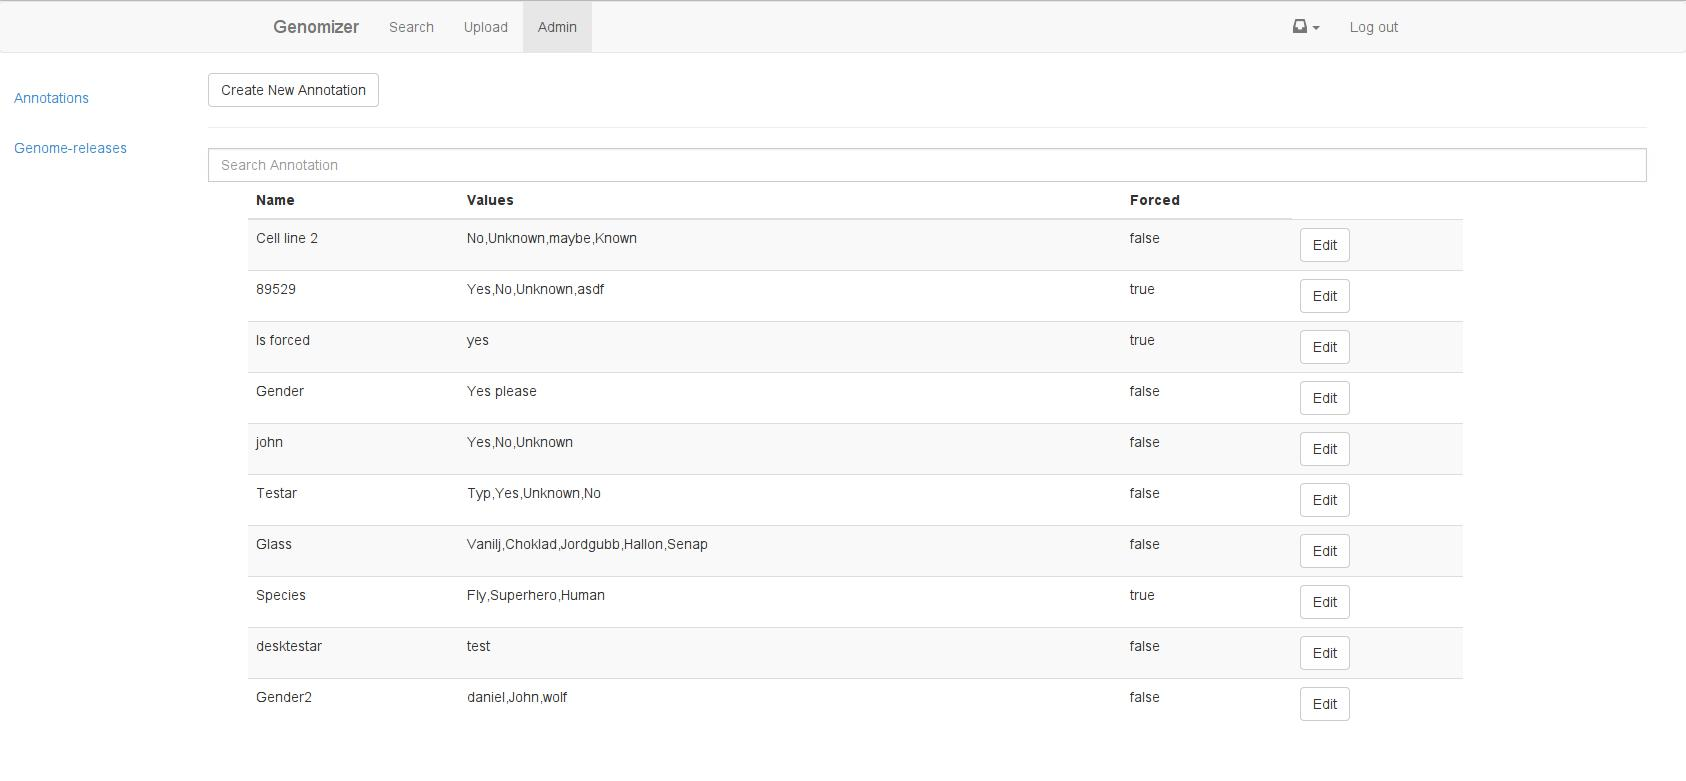
\includegraphics[trim=40 260 45 50, clip, width=0.8\textwidth]{web_SysadminAnnotationView.jpg}
 \caption{The web client navigation bar.}
 \label{adm_web_annotationView1}
\end{figure}

	\item \textbf{Main views:}
A main view covers the entire page except for the navigation bar. The structure among main views is shallow and the user may freely navigate between all main views using the navigation bar. Typically a main view contains a toolbar and a set of panels. \autoref{adm_web_annotationView2} shows the administration main view.

\begin{figure}
 \centering
 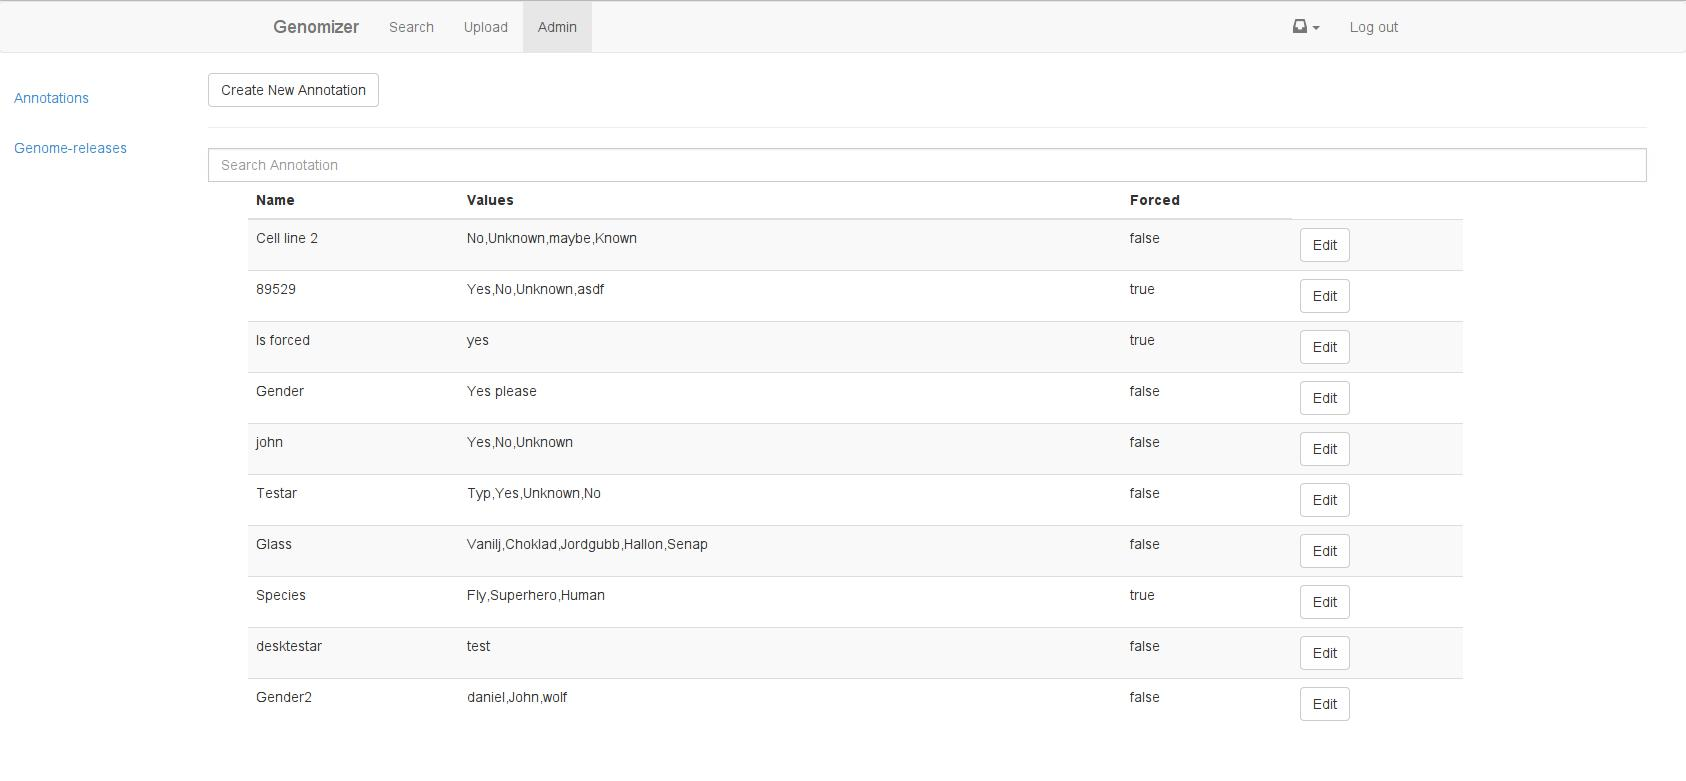
\includegraphics[width=\textwidth]{web_SysadminAnnotationView.jpg}
 \caption{The web client administrator main view.}
 \label{adm_web_annotationView2}
\end{figure}

	\item \textbf{Sub views:}
A sub view is a part of a main view. In the case of the administrator view seen in \autoref{adm_web_annotationView2}, the main view has a vertical navigation bar on the left side used to navigate between sub views, sub views may not be directly navigated outside of its main view. The user may navigate to other main views from a sub view. Except for the sub navigation bar the sub view covers the entire main view, replacing its content, as does the annotation view in this case.

	\item \textbf{Modal views:}
Modal views are opened on top of the current main view and are used for specialized operations. Modal views can be navigated to using buttons inside main views and sub views. Usually the user will be taken back to the previous view when the modal is closed but navigation in a sequence of modal views could be implemented in the future. An example
of a modal view is the login view seen in \autoref{fig:web_search_login1}.

\begin{figure}
\centering
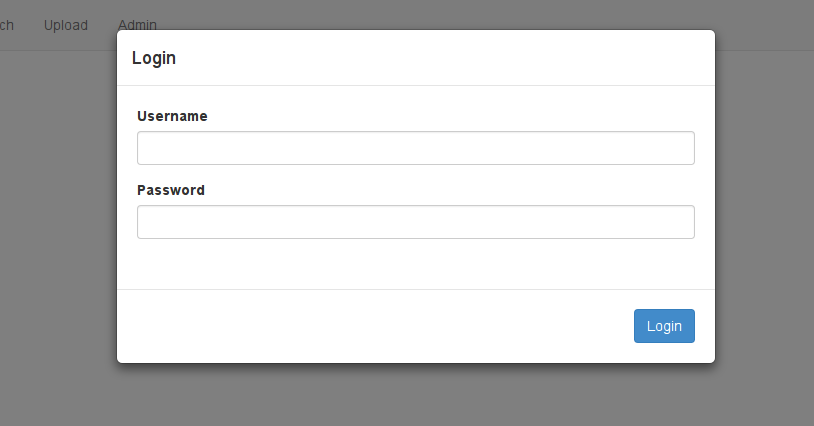
\includegraphics[width=0.8\textwidth]{web/manual/web_login.png}
\caption{The login modal.}
\label{fig:web_search_login1}
\end{figure}

    \item \textbf{Panels:}
Content that belongs together is grouped using so bootstrap panels. Main views and sub views should contain one or more panels.
    
    \item \textbf{Toolbars:}
In main views and sub views we use a toolbars where operation controls available to the user are presented, for example, add and search experiment functionality in the upload view.
    
    \item \textbf{Popovers:}
Elements that belong to a view but have no need to be visible at all times are shown in bootstrap popovers. Popovers that do not belong to a specific view may be placed in the navigation bar, that is, the main menu.
\end{itemize}

\subsubsection{Colors}
Grayscale colors are mostly used, black or dark gray is used for text, icons and borders while white or light gray is used for backgrounds. Colors of different hues are used to distinguish elements from each other and to highlight important elements. Colors with high saturation are reserved for smaller elements while colors with lower saturation can be used regardless of element size. Light gray of varying brightness may also be used to highlight or distinguish elements.

\subsubsection{Icons}
Buttons that perform actions should always contain an icon as well as text so that the experienced user may more quickly desired actions by identifying buttons at a glance instead of having to read the button text. 

\subsubsection{Batching}
For operations performed on objects that there are multiples of e.g. experiments or files, let the user perform these operations on multiple objects at the same time in cases where it makes sense using checkboxes.

\subsubsection{Processing}
The interaction flow of the processing is adapted from the actual processing 
steps in order to help the researchers by increasing usability through providing
a well-known but more optimized approach.

After having chosen an experiment for processing and entered the processing 
view, the user can choose the processing steps wanted and enter the correct
files and parameters for each processing step as shown in .

\subsubsection{System administration}
The admin page is built up by a number of components: the main view, the side bar, the create annotation view, the edit annotation view and the genome-release view. The first one is the main view which consists of a sidebar and an empty div-tag. The empty div-tag is then replaced with the annotation list view which has a Create new annotation button and a list of the available annotations on the database with an option to edit. 

When the user clicks on for example Create New Annotation, the div tag in the main view is replaced with the create annotation view. The same goes for the Edit buttons on each annotation. This way we only have to render that specific div-tags current information and the sidebar is unaffected. 

The design is made so that the user should be able to avoid mistakes. For example in the create annotation page the user is not able to create an annotation without filling in all the fields. Futher more the field for Items in drop-down list is disabled if the user don't choose Drop-down list as the annotation type. 

In the Edit annotation view the same principles apply, but also there is a Delete Annotation button on this page which will delete the entire annotation from the database.For that reason we decided to ask if the user is sure of this action and of course made the button red.

The back buttons on the different views work as one would expect and the sidebar option Annotations takes the user back to the main adminview.

The sidebar item ''Genome-releases'' takes the administrator to the page for adding and editing genome-releases. This page have the same look and feel as the previous. The delete buttons are red and will prompt a confirmation-popup. 

The ''Select files to upload'' will as expected open the file explorer and the user chooses files according to normal operativesystem standards, then the ''Upload'' button will prompt the user for information about the files such as species and genomeversion before uploading. 

\FloatBarrier

\section{Android}
%\subsection{Interaction Design}

%The design of the Android application is based on the design proposal suggested by the design team and our aim has been to recreate that look and feel. We did, however, find it necessary to take into consideration some of the Android specific design paradigms which distinguish Android applications from other smart phone platforms. For instance, the design put forth by the design group did not include a so called action bar   to the upper part of the user interface which are used for navigation. However, since these are fundamental to the structure of any Android application, we were inclined to include this feature as a substitute for the slide-in menu described in the original design.

%In the following sub-sections, we will attempt to explain our design desisions.

The \appName\ \textit{Android} application was designed to allow for a quick search of the database while on the move. It also makes it possible to start processes in advance so that the data is ready when further work and analysis is to be done. The application will also provide a way to continuously view the status of active processes on the server. 

The application was designed in close collaboration with the \term{iOS} application in order to provide a consistent experience on both plattforms.  We did, however, find it necessary to take into consideration some of the \textit{Android} specific design paradigms which distinguish \textit{Android} applications from other smart phone platforms. In this section the layout and design decisions will be described.


\subsection{Login view}
There are two textfields available for the user to type username and password and a button to click when user is ready to log in.
This is a popular layout for many login screens and thus a design many users are familiar with.


\begin{figure}[ht]
\addScaledImage{0.2}{figures/and_login.png}
\caption{\footnotesize Login view}
\label{fig:and_login}
\end{figure}
\FloatBarrier

\subsection{Search view}
The design illustrated in \refer{fig:and_search} show the search view, 
which is also the view the user is presented with upon successful login.
The search annotations are displayed in a list and it is easy to learn how to search.
Scroll bars are used for multiple options and textfields are used for free text. 
At the bottom of the view there is a button to press in order to start the search.

\begin{figure}[ht]
\addScaledImage{0.2}{figures/and_search_regular.png} 
\caption{\footnotesize Search view}
\label{fig:and_search}
\end{figure}
\FloatBarrier

\subsection{Search result view}
The design illustrated in \refer{fig:and_result} show the search result view. 
The result is shown in a list, sorted by experiments. The list displaying search results is large to facilitate usage for user and to take advantage of the screen space. 
It is easy to learn how to navigate the list. 
Scrolling is available if the list is long and if the user clicks on an experiment they are redirected to the experiment view displaying more information about that experiment.

\begin{figure}[ht]
\addScaledImage{0.2}{figures/and_search_result.png} 
\caption{\footnotesize Search result view}
\label{fig:and_result}
\end{figure}
\FloatBarrier

\subsection{Experiment view}
The design illustrated in \refer{fig:and_experiment} shows more information about a specific experiment. 
All files associated with the experiment is displayed here and sorted by type (raw, profile and region).
The button \click{Go to process} at the bottom takes the user to the process view, where the user can process all raw files associated with the experiment.
If no raw files should exist, the button will be disabled.

\begin{figure}[ht]
\addScaledImage{0.2}{figures/and_result_experiment.png} 
\caption{\footnotesize Experiment view}
\label{fig:and_experiment}
\end{figure}
\FloatBarrier

\subsection{Search settings view}
The design illustrated in \refer{fig:and_search_settings} is showing the view for search settings. 
This is a way for the user to select annotations to be displayed in the search result view.
The user can select annotations by checking the checkbox next to the annotation name.
The user can also select on how to sort the experiments.
This functionality gives the users the possibility to design the search result view the way they want to have it, which often is appreciated. 

\begin{figure}[ht]
\addScaledImage{0.2}{figures/and_search_select_visible_annotations.png} 
\caption{\footnotesize Search settings view}
\label{fig:and_search_settings}
\end{figure}
\FloatBarrier

\subsection{Process view}
The design illustrated in \refer{fig:and_processing_view} is showing the view for processing. 
This enables the user to start a process from raw to profile. The only selectable input files are the ones that exist in the experiment.
The \click{Parameters} button enables the user to change the \verb!Bowtie! flags.
The plus icon in the action bar adds a new entry, and the cross removes the associated entry.

\begin{figure}[ht]
\addScaledImage{0.2}{figures/and_processing_view.png} 
\caption{\footnotesize Processing view}
\label{fig:and_processing_view}
\end{figure}
\FloatBarrier

\subsection{Active processes view}
The design illustrated in \refer{fig:and_active_processes_view} is showing the view for active processes on the server. 
The user is automatically navigated here when the \click{Process} button in the process view is clicked.
The user can here choose to remove any process on the server.

\begin{figure}[ht]
\addScaledImage{0.2}{figures/and_process_status.png} 
\caption{\footnotesize Active processes view}
\label{fig:and_active_processes_view}
\end{figure}
\FloatBarrier

\FloatBarrier
\section{iOS}

Focus has been on making a nice looking application with an intuitive workflow and to follow the iOS design principles. Some of the design decisions are motivated in the text below.

\subsection{Navigation bar}
A navigation bar is used to make access to different main functionalities available at all times. Big and clear icons are used to show the user which view they all represent. It is also possible to simply swipe between the different views to increase the speed of which the advanced user can use the system.

\subsection{Login Screen}
The login screen has two responsibilities; to make a nice first impression and to make it easy for the user to login. The design is kept simple and clean to avoid distractions.

\subsection{Search View}
The search view is designed to be usable for both advanced and new users. A list with available annotations is displayed to make it easy to do basic searches fast. Some annotations can only be selected with a picker view, while others are edited by typing free text. The reason for the occurance of the picker views is to simplify searches and help the user to make correct search requests. For example, the sex of an individual can only be male, female or unknown. Other values for the sex annotation would be nonsence! The search button disappears when no annotation is selected to decrease the chance of user sending empty searches and to increase the understanding of the switches. 

\begin{figure}[ht]
\addTwoImages	{ios_search1.PNG}{a}
		{ios_search2.PNG}{b}
\caption{The search screen.}
\label{fig:ios_search2}
\end{figure}
\FloatBarrier

Each annotation has a corresponding switch button as seen in \refer{fig:ios_search2}a-b. The button determines if the annotation should be included in the search request. This make it easy to make small changes to the search, while not clearing the annotation values.

The advanced user can customize the search query sent to the server. This gives the user the possibility make more complex search queries and possibly make use of already accuried PubMed-search skills.

\subsection{Search Result View}
The main purpose of the search result view is to give an overview of the search results. The challenge with this view was to summarize large amount of information in a small area. The small screen of the iPhone made it impossible to have columns for each annotation. Instead a decision was made to group the files by experiment as seen in \refer{fig:ios_searchResult2}. The table with the experiments will only expand vertically, both when the number of shown annotations and the number of experiments grows. Thus, the user never has to scroll sideways which would be awkward.

\begin{figure}[ht]
\addScaledImage{0.30}{ios_result3.PNG}
\caption{The search result view.}
\label{fig:ios_searchResult2}
\end{figure}
\FloatBarrier

The user can choose which annotations to display in the result view. This gives the user the possibility to only show the annotations which are interesting at the moment. 

The files view (see \refer{fig:ios_files2}a), which is shown when the user selects an experiment, only contains the filename of the files in the specific experiment. The annotations is not shown in this view to avoid information overload and to give the user a good overview of the files. The purpose of the plus-symbol next to each file is to add as many files as the user wish to use when selecting processes. More information can be seen when the circled 'i' to the left of the filename is tapped, an example of this can be seen in \refer{fig:ios_files2}b. 

\begin{figure}[ht]
\addTwoImages	{ios_process_files.jpg}{a}
		{ios_files2.PNG}{b}
\caption{The file view.}
\label{fig:ios_files2}
\end{figure}
\FloatBarrier


% The functionality of the Convert files button can be reached from other views, but was added to this view as well to improve the workflow. Instead of first selecting the files, then going to the Selected files view and initiate the convertion from there, the user can quickly convert files directly from the search results.

%\subsubsection{Selected Files}
%The selected files view can be seen in \refer{fig:ios_selectedFiles2}a. The files are grouped into four categories: raw, profile, region and other. This is done by showing each type of files in its own tab located at the top of the screen. The reason for this is to avoid the possibility to select files of different types since the tasks to perform are file type specific. It also gives a better overview of the files when only one type is shown instead of showing all files at the same time. The files are also grouped into respective experiment they belong to. This is done to avoid confusion of what file belong to which experiment with similar filenames etc. Additionally, the top navigation bar menu is following the iOS design guidelines. 
%
%When at least one file is selected with the switch next to it (see \refer{fig:ios_selectedFiles2}b) a button will appear at the bottom of the screen letting the user choose a task to perform with the file by leading to the select task menu, as seen in \refer{fig:ios_convertParameters}a.
%
%\begin{figure}[ht]
%\addTwoImages	{ios_selected1.PNG}{a}
%		{ios_selected2.PNG}{b}
%\caption{The selected files view.}
%\label{fig:ios_selectedFiles2}
%\end{figure}
%\FloatBarrier


\subsubsection{Create processes}
The view to create a process is focused on the user's current workflow. The user wants to use the selected files from the files view as input and then select a specific process on those files, which creates output-files to be used as input-files in another process. This creates a sequence of processes which the server will execute one process at a time. Moreover each input-file for a process will be executed parallel with eachother. The input-files and the output-files are separated by the process which will be executed on the input-files. To make it easy to understand what will be executed on each step of the sequence the separator between input-files and output-files is the name of the process and an arrow from the input-files to output-files. The color of a output-file will have the same color as its corresponding input-file to track a file's conversion-process, from start to finish, see \refer{fig:ios_creating_process}a-c. 



\begin{figure}[ht]
\addThreeImages {ios_empty_make_process.jpg}{a}
	{ios_one_process.jpg}{b}
	{ios_many_process.jpg}{c}
\caption{Creating a process}
\label{fig:ios_creating_process}
\end{figure}
\FloatBarrier

\subsubsection{Processes}

As visible in \refer{fig:ios_processingStatus}, we chose to build the processing status view with a simple tableview, to make it dynamic and easy. We also think this gives the user the best possible overview of current processes. The status is color coded to make it as easy as possible for the user to see which processes are in which state.
\begin{figure}[h]
\addScaledImage{0.30}{ios_processes1.PNG}
\caption{The process status view.}
\label{fig:ios_processingStatus}
\end{figure}
\FloatBarrier

\subsubsection{Alerts}
Alerts are simple banners animating down from the top to give the user a headsup of what is going wrong and what is going the way it is expected. The user can tap the banner to dismiss it or if nothing is done it will animate away in 2 seconds. The banners were introduced to not stop the user with prompts which the user has to react with to be able to further use the system. A red banner, as seen in \refer{fig:ios_alerts}, indicates an error and a white with a green icon, indicates something went as expected. The colors are used to allow the user to just notice which color pops down and give them somewhat of an understanding of what is going on. without having to read the text every time.
\begin{figure}[ht]
\addScaledImage{0.30}{ios_alert1.PNG}
\caption{Examples of alert}
\label{fig:ios_alerts}
\end{figure}
\FloatBarrier





\chapter{Architecture design}
%An overall look at how the architecture of the systems is designed. Communication diagrams and how the different parts interact with eachother. Directed towards developers.

To get an understanding on how the system is designed as a whole, this chapter will try to explain the architecture of the system on a more broad level and design choices that is to expensive to change at the current point in the project.

\label{chap:com_latexoverview}
\section{System overview}
%Things that people perceive as hard to change;[6] since designing the architecture takes place at the beginning of a software system's lifecycle, the architect should focus on decisions that “have to” be right the first time, since reversing such decisions may be impossible or prohibitively expensive.
The \appName\ is a server-client architecture. It consists of four different clients: a web client, a desktop client and a two kinds of mobile clients. The mobile clients are implemented in \textit{Android} and \textit{iOS}. The server side consists of three components, a web server that acts as a proxy, a \textit{Java} server that connects to the final component a \textit{postgresql} database.

The web server is a \textit{Apache} system in the current implementation.

\begin{figure}[h!]
\begin{tikzpicture}[ 
	font=\sffamily,
	every matrix/.style={ampersand replacement=\&,column sep=0.5cm,row sep=0.5cm},
	db/.style={cylinder, shape border rotate=90, draw, fill=orange!40, minimum height=2cm, minimum width=1.5cm},
	server/.style={rectangle, draw, fill=orange!40, minimum height=1cm, minimum width=2cm, font=\ttfamily\footnotesize},
	webb/.style={rectangle, draw, fill=blue!40, minimum height=1cm, minimum width=2cm, font=\ttfamily\footnotesize}, 
	mobile/.style={rectangle, draw, fill=red!40, minimum height=1cm, minimum width=2cm, font=\ttfamily\footnotesize},
	desktop/.style={rectangle, draw, fill=yellow!40, minimum height=1cm, minimum width=2cm, font=\ttfamily\footnotesize},
	apache/.style={rectangle, draw, fill=green!40, minimum height=1cm, minimum width=2cm, font=\ttfamily\footnotesize},
	both/.style={<->,>=stealth',shorten >=1pt,semithick,font=\sffamily\footnotesize},
	to/.style={->,>=stealth',shorten >=1pt,semithick,font=\sffamily\footnotesize},
	every node/.style={align=center}]  
\matrix{
	\node[webb] (webb) {Web}; \&
	\node[desktop] (desktop) {Desktop}; \&
	\node[mobile] (mobile) {Mobile}; \\
	\& \node[apache] (webServer) {Web server\\ Proxy}; \& \\
	\& \node[server] (genomizer) {Genomizer}; \& \\
	\& \node[db] (db) {DB}; \& \\
	};
	
	\draw[both] (webb) -- (webServer);
	\draw[both] (desktop) -- (webServer);
	\draw[both] (mobile) -- (webServer);
	\draw[both] (webServer) -- (genomizer);
	\draw[both] (genomizer) -- (db);

\end{tikzpicture}
\caption{Overview of the system architectur}
\label{fig:archOverview}
\end{figure}

The connection to the server from any client goes through the web server which acts as a proxy aswell. This to insure a \textit{SSL} connection between the web server and the clients and a regular connection between the server and web server. The proxy protects the web client from \textit{XSS} (Cross site scripting). 

All of the clients use the \term{RESTful} protocol where the message body consists of a \json\ object.
These messages are requests that gets passed through the web server to the \appName\ server. The \appName\ server communicates with the database to perform the request. Then it generates a response following the \term{RESTful} protocol. The \term{RESTful} protocol is used to promise that the server will be state-less. State-less meaning that a request from a client can not lock the server for other clients requests. 

The different requests that can be sent to the server are defined in the Appendix \fullref{chap:com_api} that goes into deeper detail about the API.

The architecture of the system can be seen in Figure \ref{fig:archOverview} where the clients are the colors blue, yellow, and red. Web server is green and the \appName\ server and its database are colored orange.

\subsection{Genomizer clients}

All the clients that are part of the \appName\ service are implemented using the architectural design pattern MVC (\texttt{Model View Controller}). This pattern is based around keeping the logic and data separate from its representation and user interface. The basic idea is shown in figure \refer{fig:MVCimage}.

\begin{figure}[htb]
\addImage{MVCstuffarch.png}
\caption{Basic MVC pattern.}
\label{fig:MVCimage}
\end{figure}

 The view will contain lists of experiments and annotations, data regarding process status, and other information. It will also present the user with windows and buttons that present and allow data to be manipulated. When a user interacts with the graphical interface the action will be handled by the controller using listeners. This in turn modifies the model; representing the data and information, as well as the operations available on it. 
 
 For this project a communication part is also necessary; often as a part of the model. As mentioned in \refer{chap:com_latexoverview}, the communication is performed via a \term{RESTful} protocol using \json\ requests and responses. \json\ is used because it is easy to parse and is directly compatible with the standard frameworks used in the web client.
 
 The advantage of this approach lies in the separation of the interface- and logic-code; allowing one to be more easily replaced or modified. In our case the communication data and interface can be kept the same, while the client representation of it can be changed freely.
 

\subsection{Genomizer server}
The server is devided up in three main components, the front end, the data storage and the processing.

The front end consist of a handler for the \term{API} requests mentioned above. The handler interpret incomming request and passes them through to either processing or data storage depending request type.

Data storage makes up the back-end of the server. Its purpose is to communicate with file system and the database to return the correct information that was requested by the front-end.

The processing does the processing of files and convertation between file types. Processing is a heavy workload on the server and has to be scheduled for both time of day and  parallel processing.

\refer{fig:com_systemoverview} shows a simple flow diagram which describes how the client and server
 communicates. The particular example shows the data flow when the client process a file.
 In the figure the front-end is the data transfer and communication node while data storage makes up the database node and processing the final process node.

\begin{figure}[htb]
\addImage{com_systemoverview.jpg}
\caption{A simple flow diagram for the system}
\label{fig:com_systemoverview}
\end{figure}

Every request the client does creates a non persistent connection to
the server. When the server receives a request it checks which kind of
request it is and routes it to the communication part of the server.

When the request is routed to communication a specific command is
created. The command is an object which consists of information from
the \term{RESTful}-header and \json/ body sent from the
client. The command is then parsed and sent to different parts of the
server, usually the database first, which returns information from a
\term{SQL query}. Depending on the requests this information can later
be used, for example, to process a file or be sent back to the clients
directly.

The clients are always going to receive a response code after each
request, but in some cases the respond also contains a \json/
body with information which can be shown to the user. This is the case
for requests like $getAnnotations$. The response can also contain
error messages, describing what went wrong when executing the command.

After a client receives the response the connection with the server is
closed and a new is opened with the next request.






\chapter{System design}
%A more indepth look at how the system is designed with UML- and class-diagrams. Directed towards developers. Start with subsubsection here.

A more indepth look at how the system is designed with UML- and class-diagrams. It is divided into two main sections for the server and clients. The client section contains the different clients. After that follows the server section that is divided into different parts that makes up the whole server. 

%\section{Clients}
%Here is an explanation of the  different client system designs.
\section{Desktop application}
The desktop client is constructed around the model-view-controller pattern. It
relies heavily on action events being performed in the graphical interface which
is then handled by the controller. The model is the part handling the
communication and the storing of important information such as ongoing downloads
and the user token (used for communication authorization). In
\refer{chap:des_appendix} a UML-diagram of the desktop client is presented. 

\subsection{View}
The view of the \appName\ Desktop client is constructed with tabs. There are 5 different tabs. These are Search, Process, Upload, Workspace and Administration.

Each tab in the view is represented by its own java class. The QuerySearchTab class which represents the search tab can display both a search view and a results view. It uses the QueryBuilderRow class to construct the rows in the query builder which is used to construct search queries. The QueryBuilderRow class represents a row in the query builder and each row is dynamic and can change accordingly to user interaction. The search results are also implemented in the QuerySearchTab and the results are displayed with the TreeTable class which is further described in the utilities section below.

The UploadTab Class represents the upload view of the GUI. It has functionality to both upload a file to an existing experiment (which is separately handled in the UploadExistingExpPanel) and to create and upload a new experiment.

The ProcessTab class represents the process view in the GUI. It contains a list where files to be processed can be stored and a large number of processing parameters which can be changed by the user. There process tab also contains a console for displaying direct feedback on processes and an area which contains the status of all current processes which are being handled on the server. The later can be updated manually with a refresh button.

The major part of the WorkspaceTab class consists of a TreeTable which holds all the experiments and the corresponding data which the user has added to the workspace. Then there is also five buttons implemented which allows the user handle the data in the TreeTable. These buttons are Remove from workspace, Delete from database, Upload to, Download and Process. The TreeTable view can be changed to a view which displays all current and completed downloads. This is made using a tabbed pane containing the TreeTable view and the Downloads view.

\subsection{Model}
The model part of the system contains methods for doing most of the logic in the system. For example there are methods for sending login requests and for downloading files. There are separate classes for downloading and uploading files as well as a class for regular communication with the server called Connection. New connections are created with the ConnectionFactory class. The model also acts a storage for importating information such as the user token and list of ongoing downloads and uploads.

The AnalyzeTab Class is not yet implemented.

\subsection{Requests}
The Request package contains the Request class , the RequestFactory and all the classes that extends the Request class. Request is the super class and can make a JSON package that all the other Request classes can use. All requests must have a name, type and an URL, but can consist of more information. For example LoginRequest also has username and password. RequestFactory is a class that can create all objects from all types of requests. It is a way to easily create all requests from the same place.


\subsection{Response}
This package consists of all types of responses that the server can send to the client-program. There is a class named Response that all the other response classes extends from. For example there is a response class for the login request called LoginResponse. All types of responses have different properties. There is also a class ResponseParser that can parse the responses so that the important information can be taken out of a JSON-package. This information can then be used to tell the client program what should happen next in the user interface.


\subsection{Controller}
The controller part of the system consists of ActionListeners for the different buttons and functionalities in the view. For example there are Listeners for searching, downloading and processing. The Controller class has access to both the view and the model and acts as a middle hand between those two parts of the system. Usually a Listener in the controller reacts upon user input and then modifies the model and gives information about the change to the view.


\subsection{Utilites}

There are several classes which represents different data in the system. There are classes for experiment data, file data and annotation data. For example when a search response is received from the server it is parsed into experiment data and the experiment data contains file data and annotation data. There is also a class representing Process feedback data.

The TreeTable class represents the table which displays experiment data, annotation data and file data in the Search and Workspace tabs. It is specially constructed to handle the data classes and it allows vertical sorting.

\subsection{System Administration}
%Till Sysadmin!
The system administration is developed separately from the rest of the GUI, and therefore has a slightly different way of communicating.

\textbf{Communication with the Server}


All communication between the server and the system administration tab follows a line of steps. See \refer{fig:adm_com_view} below.

\begin{enumerate}

  \item An event is triggered by the user clicking something.
  \item The listener for the active tab receives the event and sorts out which type it is, and calls the appropriate method in the \textit{SysadminController} class.
  \item The \textit{SysadminController} has the connection to the \textit{Model}, and calls the associated method there.
  \item The \textit{Model} creates the corresponding request for the server, and then creates a new connection.
  \item The \textit{Connection} receives the request from the \textit{Model} and sends the request to the server.


\end{enumerate}

If the event triggers a request for data, the \textit{Model} will use a parser to parse the data before sending it back to the GUI to present it to the user.


\begin{figure}[hbt!]
\addImage{adm_comm_view.png}
\caption{Communication Overview}
\label{fig:adm_com_view}
\end{figure}

\textbf{A communication example}

As a more detailed example of Figure \ref{fig:adm_com_view}. Assume that the user clicks the 'Genome Files' tab in the 'ADMINISTRATION' tab. This will trigger an event (1) to be handled by the \textit{SysadminTabChangeListener} (2) who will receive the event and execute the desired behavior of the tab, which is to directly show the available genome releases. This is done by sending a request to get available genome releases to the server and then parse the response. 

In order to contact the server the \textit{SysadminTabChangeListener} (2) calls the \textit{SysadminController} (3) who uses a reference to the class \textit{GenomeReleaseTableModel} (4) to call the method \textit{getGenomeReleases()}. \textit{getGenomeReleases()} will create a \textit{GetGenomeRequest} using the \textit{RequestFactory}. The request is then sent to the server through the \textit{Connection} class (5). The response from the server is passed to the \textit{ResponsParser} that parses the JSON respons into wanted \textit{GenomeReleaseData[]} object. The genome release array is return all the way back to \textit{SysadminController} (3) which updates \textit{GenomeReleaseTableModel} with the new \textit{GenomeReleaseData[]} and at last lets the GUI know that the data has changed through a new event (1). This will trigger the GUI to repaint and show the available data.

\textbf{Building the Administration Tabs}


All tabs under the Administration tab are built in a similar fashion and then added to a
JTabbedPane in the \textit{SysadminTab} class. Each tab has it’s own package containing 
all classes associated to the particular tab. All tabs are also built step by step by 
using smaller methods creating panels and components. Each tab has at least one main 
listener that is added to all components that require listeners. Once an event is triggered 
in a tab the corresponding listener simply use a switch case based on button/tab names 
to decide which action to take. The main listeners have an instance of the \textit{SysadminController }
to be able to further handle requests from the user and send them forward to the \textit{Model} if neccessary.

\textbf{Important classes}
The system administration part of the desktop application depends on quite a few classes and is based loosely on the model-view-controller design pattern. Here follows a list of the most important classes and a short desciption of their function and responsibilities.
\begin{itemize}
\item SysadminController - Handles the communication between the SysadminTab and the GenomizerModel. The SysadminController creates all ActionListeners for the buttons in the different views. Some minor commands are handled within the sysadmin package, but user commands requiring input or output from the server are recieved from the different components of the SysadminTab and sent to the GenomizerModel which converts them to Request objects and sends them on to the server.
\item SysadminTab - Builds all of the different views that are displayed within the system administration tab. When creating the views it also adds the ActionListeners to the buttons and fields. It also holds a reference to all of the view components it has created so that information can be sent to and from the controller when needed.
\item The listener classes - These are added to all of the components of the view that the user can interact with. When an action is performed, the listener performs the action that is assigned to the command string associated with the action. All of the command strings are stored in the SysStrings class for easy access.
\end{itemize}


\textbf{Button and Tab names}

To simplify the naming of buttons and tabs a class called SysStrings is used. All buttons or tabs are named here and then this class is used when setting the actual names. This is to avoid hard code as well as making names easy to change and hence more dynamic.

\subsection{Flow of the system}

The sequence diagram in \refer{fig:des_download-sequence} describes the flow of the system when the user presses the download file button and the diagram in \refer{fig:des_login-sequence} describes how the desktop clients reacts to a login.

\begin{figure}[htb!]
	\addImage{des_download-sequence.jpeg}
	\caption{UML sequence diagram of downloading a file}
	\label{fig:des_download-sequence}
\end{figure}

\begin{figure}[htb!]
	\addImage{des_login-sequence.jpeg}
	\caption{UML sequence diagram of login}
	\label{fig:des_login-sequence}
\end{figure}
\FloatBarrier

\FloatBarrier

\section{Web application}
This section describes the design of our system, first with a system overview and then with more indebth information about our tabs.
\subsubsection{How our web application works}
%figure x5
\begin{figure}[h]
\centering
\includegraphics[width=1\textwidth]{web_system_backboneWebapp.png}
\caption{\label{fig:web_system_backboneWebapp}A general build of a backbone webapp.}
\end{figure}

\refer{fig:web_system_backboneWebapp} shows how a backbone\cite{web_1} web application works in general. We have a user, that interacts with a browser. A browser renders the DOM of our web application. How it does this is up to the browser. Different browsers might display it differently. Models and Collections will talk to the server to update themselves. For example, our \textit{Experiments} collection will retrieve experiments from the server and update itself with a call to it’s fetch() method. Out of the components that go into this figure, we are in charge of and only capable of changing a few of these; \textbf{View}, \textbf{Template}, \textbf{Collection} and \textbf{Model}. See the Backbone section of Frameworks in section \ref{sec:web_frame} more information.

\subsubsection{System overview}
%figure 2
\begin{figure}[h]
\centering
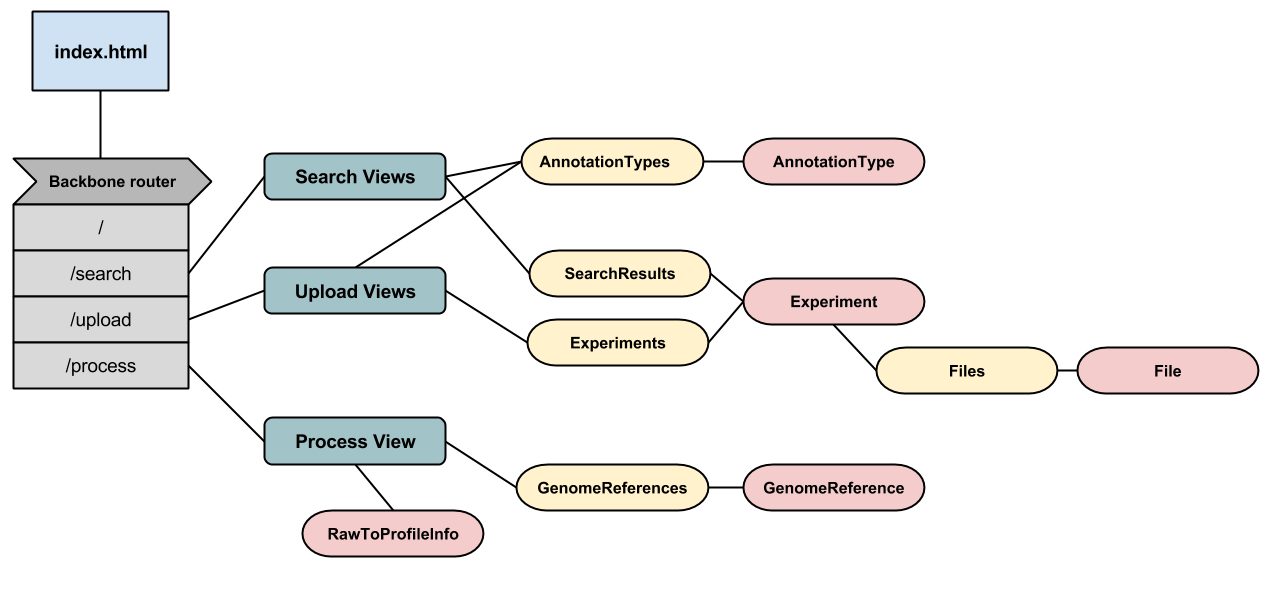
\includegraphics[width=1\textwidth]{web_system_overview.png}
\caption{\label{fig:web_system_overview}Overview of the relations between the different javaScript prototypes in the system.}
\end{figure}

Since our app is built using Backbone\cite{web_1}, our app is divided into the parts \textbf{Misc}, \textbf{Views}, \textbf{Collections} and \textbf{Models}. In \refer{fig:web_system_overview}, we can see the system overview. The \textbf{views} are the parts in green, the \textbf{collections} the parts in yellow and the \textbf{model} the parts in red. The parts in grey represent the router which belongs in our Misc category. It is responsible for rerouting links. For example, when a user clicks the search tab, the router navigates to /search, but instead of loading the whole /search over the page we are currently on, our router will open our search tab below our navigation bar. The \textbf{Misc} category also holds our Main.js, which is in charge of setting up and starting the app.

\subsubsection{Search}
The search tab has three views, the main one being \textit{Search}, which acts as a container for the \textit{SearchResultsView}and holds the search input field and the various buttons displayed. The \textit{SearchResultsView} handles rendering the annotations and the \textit{ExperimentViews}, where one \textit{ExperimentView} is created for every experiment returned from a search. The actual data retrieved is stored, by experiment, in \textit{Experiment models}. To organise this data, we have a collection to contain all the experiments retrieved, called \textit{SearchResults}.
 
%figure bla bla/lalalallala
\begin{figure}[h]
\centering
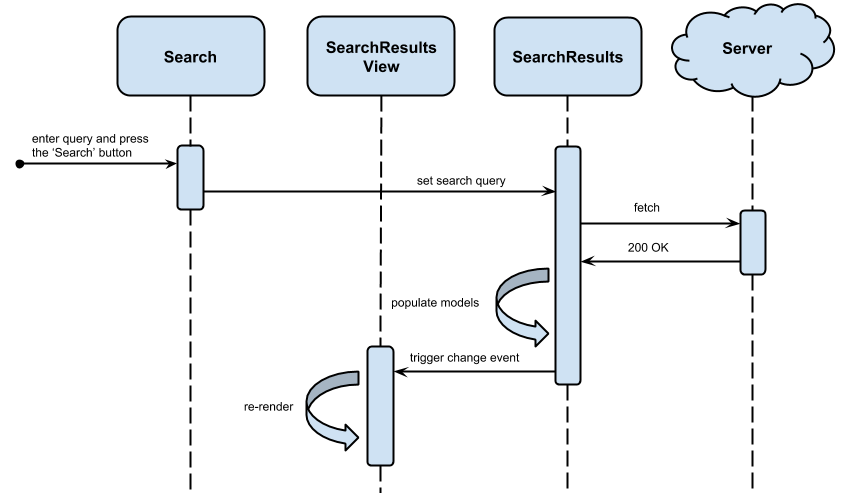
\includegraphics[width=1\textwidth]{web_system_sequenceDiagram.png}
\caption{\label{fig:web_system_sequenceDiagram}a sequence diagram showing what happens when a user enters a valid search query and results are fetched.}
\end{figure}

In \refer{fig:web_system_sequenceDiagram} is a simple sequence diagram for the search tab. If a user enters a query in the search field and then presses the search button, the \textit{Search} view will update the \textit{SearchResults} collection to have a new query. Once \textit{SearchResults} has a new query, it will try to fetch search results corresponding to the query from the server. If successful, new experiment models for every experiment retrieved will be created and set in the \textit{SearchResults} collection. \textit{SearchResults} then triggers a ‘change’ event that \textit{SearchResultsView} listens to. When that event occurs, \textit{SearchResultsView} knows that \textit{SearchResults} has been changed, and re-renders itself.


\subsubsection{Upload}
The upload tab has three main views, the main one being Upload, which acts as a container for the ExperimentView’s and holds the search input field and the various buttons displayed. Each ExperimentView handles rendering the AnnotationsForm and the FileUploadList, where one ExperimentView is created for every experiment the user inputs. The actual annotation data is stored by the \textit{Experiment} model. Files are stored as a \textit{Files} collection in the \textit{Experiment} model. \textit{Experiments} are in turn stored in the \textit{Experiments} collection.
\subsubsection{Process}
Processing has genomeReferences to match with the specie the processing is being done on. Other that that the processing part is mainly a graphical interface with not that much systemDesgin in.

\subsection{System administration - Web}
The system administration part of the web client is developed using the same tools and frameworks as the rest of the web client.
This admin part of the system is made up of view classes, model classes and collection classes. The classes are described below:

\subsubsection*{Classes used by all views}

\strongTerm{Gateway} - this is a model class used solely for communication with the server. It is a static class in the sense that it doesn't have to be created. It only needs to be included and then its functions can be called immediately without having to be instantiated. The gateway class retrieves the URL from the main JavaScript file this way the URL only needs to be declared once. The URL can then be fetched by any class that includes the Gateway class.

\strongTerm{SysadminMainView} - the main view for the admin tab, this view is used together with every other admin view. It contains a sidebar menu used to navigate between different admin views.

\subsubsection*{Classes used to handle annotations}

\strongTerm{Annotation} - this is a backbone model that represents an annotation. An annotation consists of three fields. A name, a list of values and a forced field. The name simply specifies the name of the annotation. The list determines whether this annotation is a drop-down list, or a free-text field. If the list contains one element called free-text, the annotation is a free-text field. Otherwise it is a drop-down list with the values in the list. The forced field determines if
the annotation has to be filled in by the user when a file is uploaded.

\strongTerm{Annotations} - this is a backbone collections that consists of several Annotation models. It also has a URL that it uses to fetch annotations from the server, the URL is retrieved from the Gateway class. 

\strongTerm{AnnotationsView} - this view is the basic view for displaying annotations. It has a search field and a button for creating new annotations. Pressing the button renders the newAnnotationView. 

The AnnotationsView has a child view called AnnotationListView. This way the list view can be rendered separately from the search field when the user types in searches. 

\strongTerm{AnnotationListView} - this view uses the Annotations collection to fetch all the annotations from the server and renders them dynamically in a list.
In the list is an Edit button for every annotation, the edit button will retrieve the name of the desired annotation and navigate through the router to the EditAnnotationView with the name as a parameter.
The view also has a button that will take the user to the NewAnnotationView.

\strongTerm{EditAnnotationView} - this view uses the name parameter received from the AnnotationListView to retrieve a specific annotation from the collection of annotations. It then renders the fields with the values from the annotation. This view has a button to delete an annotation. It will send a delete message to the server using the Gateway model to delete the annotation. An annotation can also be modified in different ways.

\strongTerm{NewAnnotationView} - this view is used to create a new annotation. It consists of a couple of fields and a create button. Pressing the create button renders a ConfirmAnnotationModal which displays the values for the annotation.

\strongTerm{ConfirmAnnotationModal} - this class extends the ModalAC class. It is simply used to display information that the user has to confirm. Pressing confirm creates a message using the Gateway class and sends it to the server.

\subsubsection*{Classes used to handle genome releases}

\strongTerm{GenomeReleaseView} - this view is used for viewing, adding and deleting genome releases. It contains a button ''Select files to upload'' which opens up file explorer and lets the user select one or multiple files for uploading. When the user then presses upload the UploadGenomeReleaseModal will open. Below the button the view has a table showing the current genome releases available on the server. The user can hold the mouse over files too see all files included in that genome release. A ''Delete'' button is shown next to every genome release and if pushed sends a delete request to the server through the Gateway class. 

\strongTerm{UploadGenomeReleaseModal} - this modal shows the user which files has been selected for upload and asks for information about which species and genome version they are for. Then at the press of ''Upload'' the files starts to upload and the user will see a progress bar over the complete upload progress. 

\strongTerm{GenomeReleaseFiles} - this is a collection with GenomeReleaseFile as models. It handles the ordering and filtering of its models. 

\strongTerm{GenomeReleaseFile} - this model represent a genome release and can contain multiple files in itself since one genome release is almost never just one file. This class takes case of uploading itself to the server and thereby also updates the progress bar through events that propagate up to the GenomeReleaseFiles collection. 

\FloatBarrier

\section{Android application}
The following sections describe the system design of the Android application. All functionality of the system components are described in this section. Worth noting is that the figures referred to in this section can be found further down in the document.

\subsection{System overview}
	The Android application is divided into seven \emph{packages}. These packages are \verb!default!, \verb!com!, \verb!login!, \verb!model!, \verb!process!, \verb!processStatus! and \verb!search!.
	All packages (except for \verb!com! and \verb!model!) contains one or several fragments. A \verb!Fragment! is an object that helps to modularize the code and brings more sophisticated user interfaces.

	\begin{figure}[h]
		\centering
		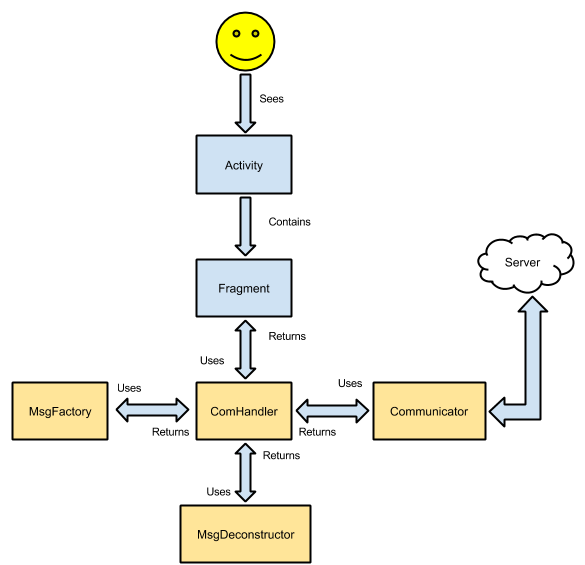
\includegraphics[width=1\textwidth]{and_system_overview.png}
		\caption{\label{fig:and_system_overview}A generalization of how the Android application works.}
	\end{figure}

	The user will interact with an activity that holds a fragment. The fragment (which contains some logic) will tell the class \verb!ComHandler! what action that should be performed. The \verb!ComHandler! will construct a message by using \verb!MsgFactory!. The message is then passed on to \verb!Communicator! which sends the message to the server with REST. The \verb!Communicator! returns the response to the \verb!ComHandler! that parses it by using the class \verb!MsgDeconstructor! and then returns it to the fragment. Hopefully, \refer{fig:and_system_overview} will bring some clarity.
	
\subsection{Package overview}
	The \verb!default! package contains the \verb!MainActivity!. This class is the base of every screen in the application after logging in. The top level navigation is handled from here.

	The \verb!com! package is responsible for communication with the server. It also contains classes and methods for construction and deconstruction of JSON.

	The \verb!login! package contains the GUI and controller for the login screen. It also enables the user to select, add, edit and delete server URLs.
	
	The \verb!model! package holds information about experiments, annotations, files etc. found on the server.
	
	The \verb!process! package is responsible for displaying processing parameters etc. for when the user wants to start a process.

	The \verb!processStatus! package shows the running, failed and succeeded processes on the server.
	
	The \verb!search! package handles searches by either selecting annotations, or by manually typing in PubMed style. It also handles the search results by displaying the found experiments in a list.
	
\pagebreak


\FloatBarrier

\section{iOS application}
The following sections describes the system design of the iOS application. The overall system design is discussed followed by a more detailed description of how the segues are controlled.

\subsection{Overall system design}
The  system is designed using the model-view-controller principle. Each view is controlled by its own controller class which reacts to user input and triggers changes in the model and updates the view accordingly.
\begin{figure}[ht]
\addScaledImage{0.3}{ios_UML2.png}
\caption{UML diagram.}
\label{fig:ios_UML}
\end{figure}
\FloatBarrier

\refer{fig:ios_UML} gives an overall image of the system design. Some classes are excluded from the figure to make it easier to get an overall idea of the system. The controller classes of the table cells and some other controller classes are not illustrated in the diagram. The non-excluded classes are described in \refer{table:ios_class_table}.

\begin{table}
\begin{tabularx}{\textwidth}{|l|X|}
\hline
\textbf{Class} & \textbf{Description} 
\\ \hline
\term{Annotation} &
Contains information about an annotation and can format the annotation name to an aesthetically more pleasing representation.
\\ \hline

\term{DataFileViewController} &
Controls the File view presented in \refer{fig:ios_files1}. It contains a reference to an experiment and lists all its files in a table.
\\ \hline

\term{Experiment} &
A class that contains information related to an experiment, as well as its files.
\\ \hline

\term{ExperimentDescriber} &
Generates a description of an experiment using annotations chosen by the user.
\\ \hline

\term{ExperimentFile} &
Contains information about a file from an experiment.
\\ \hline

\term{ExperimentParser} &
Parses experiment information from a NSDictionary to an Experiment object.
\\ \hline

\term{FileContainer} &
Contains files and sorts them by file type.
\\ \hline

\term{JSONBuilder} &
Creates different JSON requests.
\\ \hline

\term{PubMedBuilder} &
Creates a pubmed search query.
\\ \hline

\term{SearchResultController} &
A controller class for the Search Results view presented in  \refer{fig:ios_searchResult}. It configures the table which holds the information about the experiments a search resulted in. An ExperimentDescriber is used to generate a description of the experiments.
\\ \hline

\term{SearchViewController} &
A controller class for the Search view, see \refer{fig:ios_search}. It checks which annotation-fields are used and tells the JSONBuilder to generate a corresponding search query when the user presses the search button. The class also contains a advanced search to allow the user to manually enter search queries. 
\\ \hline

\term{SelectedFilesController} &
A controller class for the The selected files view shown in \refer{fig:ios_selectedFiles1}. The selected files controller contains information about files saved by the user.
\\ \hline

\term{ServerConnection} &
Sends and receives JSON objects to and from the server.
\\ \hline
\end{tabularx}

\caption{Description of some classes of the system.}
\label{table:ios_class_table}
\end{table}
\FloatBarrier

A more detailed description of these classes, and the ones not mentioned here, can be found in comments in the source code.

\subsection{Segue controll}
To avoid several segues to be executed at the same time, a segue controll package has been implemented. Instead of extending UIViewController, UITableViewController, UITabBarController and UINavigationBar the corresponding XYZ class should be used instead. An overview of this design can be seen in \refer{fig:ios_UML_segue}. This figure also includes the classes XYZDataFileController and XYZSearchResultController as two examples of such implementations.

\begin{figure}[ht]
\addScaledImage{0.35}{ios_uml_segue2.png}
\caption{UML diagram describing the segue controll.}
\label{fig:ios_UML_segue}
\end{figure}
\FloatBarrier


\FloatBarrier

\section{Server}
The design of the servers system is based around several parts. These parts consists of: communication, conversion, processing, storage and file transfer. Following is a more detailed description of each part.

\subsection{Communication}

\label{chap:com_systemdesign}
The server is based around a \texttt{RESTful} protocol where all communication is handled over non-persistent connections which the clients initiate. Since the communication is non-persistent, the server has no way of contacting clients except for responding to requests. When a client wants to connect it sends the request to a proxy, which only accepts encrypted trafic, that is then forwarded to the actual server. Once inside the server, the request is parsed, executed and a response is sent back to the proxy which forwards the message back to the client. 

To uniquely identify different logins a token is generated when a user logs in, the client now should identify itself with this token in all other requests for them to be executed. Otherwise, the server will not recognize who the client
is and therefore can't know what server commands the client has permissions to execute. 

Most commands are executed immediately when ther server recieves it, and the result is sent back as soon as the command is finished. There are however an exception to this, the process command, which is put in the back of a queue instead of being executed. The server continuously takes work from this queue and executes them as fast as it can, but due to the huge computing power requirement it cannot do them all at the same time. 

For a visual reference of the flow between the different parts of the system, see \fullref{fig:com_systemoverview}.

\paragraph*{Server Commands}

The following eleven items are the main categories of commands that can be sent: 

\begin{itemize}
	\item \textit{Connection}
	\item \textit{Experiment}
	\item \textit{Files}
	\item \textit{File conversion}
	\item \textit{Search}
	\item \textit{User}
	\item \textit{Admin}
	\item \textit{Processing}
	\item \textit{Annotation}
	\item \textit{Genome release}
	\item \textit{File upload/download}
\end{itemize}

Connection handles the \textit{Login} and \textit{Logout} commands, which are self-explanatory in their functions. There is also

\subparagraph*{Connection}

Connection handles the \textit{Login} and \textit{Logout} commands, which are self-explanatory in their functions. There is also a deprecated command which can be used, but should not, to check if the clients token is still valid or if it has expired. This was used before, but was deemed unnecessary due to this check happening on every other command as well. 

\subparagraph*{Experiment}

Used to create new experiments, update or delete existing experiments as well as retrieving information about specific experiments. Deleting or retrieving information only requires the experiments ID, whilst creating new or updating existing experiments require annotations to be specified as well.

\subparagraph*{Files}

Contains commands to create new file-posts, update or delete existing file-posts and retrieving information about specific file-posts, just as Experiment does for experiments, but for file-posts. A file-post is a database entry which keeps information about a file, as well as the path to the file. A file cannot be uploaded without having a matching file-post. When discussing files in general, file-posts and the file together will be refered to as a file. 

\subparagraph*{File conversion}

File conversion has a single command, which converts files from one file-format to another. The formats that can be converted from and to are: \texttt{.bed}, \texttt{.gff}, \texttt{.sgr} and \texttt{.wig}. 

\subparagraph*{Search}

Search is used for searching after experiments in the database, the search uses a PubMed-style query system which can be found and explained at \url{http://www.ncbi.nlm.nih.gov/pubmed}. All experiments that match the query are sent back to the client. No post-processing or ordering is done on the list ofexperiments by the server.

\subparagraph*{User}

Only contains two commands at the moment, update and retrieve information. Via the update command users can updates their password, name (fullname, not username) and email. Any other editing of users is done via the Admin category. 

\subparagraph*{Admin}

The Admin commands are the primary way of creating, editing and deleting users. Creating a new user requires a username, password, privilege level, name and email. To make editing and deleting easy to use there is also a command to get a complete list of all the usernames in the system, which together with the get user command from User, a client can get all the information about any user. 

\subparagraph*{Process}

In order to process files, the client can send a process command which is a collection of sub-commands, one sub-command for each step of the processing pipeline. Each of these sub-commands contain all the information they need to run and a list of infiles and outfiles. 

When a process command is executed, it executes the each sub-command in order. Since a sub-command might contain many input files and output files, it in turn executes on all the input files, producing all the output files before finishing, and thus, causing the process to be parallellized in each step, but each step is sequential in order.

Process also has commands to retrieve information about all the processes that are waiting, running or finished as well as canceling a running or waiting process. 

\subparagraph*{Annotation}

Annotation has two different sub-categories, annotation field and annotation value, the field is the name of the annotation and the value is the actual value. A annotation can only have a single field, but several values, and is displayed with dropdown menus in the clients. The reason for two different sub-categories is that both of the two need to be able to be created, edited, deleted separately. The retrieve only retrieves full annotations, i.e. both the name and all the possible values. 

\subparagraph*{Genome release}

Genome release is used to manage genome releases, works similarly to how file works, except a single genome release-post can have many files associated with it. 

A more detailed specification of the API can be found in \refer{chap:com_api}.

\FloatBarrier
\subsection{Data Conversion}
The \appName\ service needs to be able to convert, process and visualize data. This chapter explains how this is done in the system.

%\begin{figure}[h]
%\addImage{UMLFinal.png}
%\caption{Class-diagram  for Process}
%\label{con_UML}
%\end{figure}
	
The \texttt{RawToProfileConverter}, \texttt{Smooth}, \texttt{Step}, \texttt{Ratio} and \texttt{Bowtie} extends the \texttt{Executor} class. The different processing commands can only start the corresponding processing method on these Executors. 


\subsubsection{Executor}
The executor class, as seen in figure 5.2.1, is a abstract superclass that is an entity that is able to execute various commands. The executor class is able to run programs as well as scripts and shell commands. The commands are specified in the call to the methods in this class. \newline

\begin{tabularx}{\textwidth}{|l|X|}
\hline
\term{executeCommand} &

\term{executeCommand} is a protected method used in processing to make command line calls to external dependencies used
in the various processing steps. Firstly a \term{processBuilder} is used to ensure a safe way to execute commands, after 
that the working directory is set and the error output stream is merged with the standard output. After a command has been 
started the output stream is then recorded with the help of a Scanner object and a \term{stringBuilder} object. When the 
command has been executed the termination status is checked and the recorded string is sent back to the caller. The command 
to be executed is represented as an array of strings.
\\ \hline

\end{tabularx}

\subsubsection{RawToProfileConverter}
The purpose of the \term{RawToProfileConverter} class is that it will be used by
\term{RawToProfProcessCommand} and do all the steps in the process pipeline produce a \term{profile
file} in \term{.wig} format. These steps are done by calling external dependencies such as programs and scripts which are executed with methods that is extended from
\term{Executor} class. 
\subsubsection{Smoothing}
The term{Smoothing} class is used on a \term{profile file} to smooth down the tips, making the data result less jagged.
\subsubsection{Step}
The term{Step} class is used on a \term{profile file} to lower the file's resolution.
\subsubsection{Description of different scripts and processing steps}

\begin{enumerate}
\item \term{BowTie}: Uses the external dependency Java tool Bowtie. 
Support for Bowtie2 is implemented but not fully tested. 
Bowtie creates unsorted \term{.sam} files from \term{.fastq} raw files.
The files are created in a temporary folder with the name \filePath{result\_X}, where X is the ID of the current thread. 
All other folders created is placed inside the folder from where the files used where placed.

\item \term{sortSam}: Uses external dependency Picard and sorts the \term{.sam} file and creates a new \term{.sam} files, sorted by coordinates.
The files are saved in the same temporary folder as in the Bowtie step.

\item \term{RemoveDuplicates}: Uses the external dependency Python tool Pyicos.
Takes a sorted \term{.sam} file and produces a new \term{.sam} file with all duplicate reads removed.
It is optional to save this \term{.sam} file to the database but it is saved in the temporary directory in the mean time.

\item \term{Convert}: Uses external dependency Python tool Pyicos.
This is the final step of raw to profile conversion and uses Pyicos to convert a given \term{.sam} file to \term{.wig} file.
All intermediate files are removed except optionally the \term{.sam} file which can be returned together with the final \term{.wig} file. All saved files are moved to the given profile directory path.

\item \term{Smooth}: smooths the file and creates a large \term{.sgr} file,
converted the customers \term{Perl script} by following the algorithm they  sent
us. This makes it more efficient. Puts the files in a folder called
\filePath{smoothing}.

\item \term{Step}: Takes the smoothed \term{.sgr} file and takes samples from it
with a specified interval and creates a smaller \term{.sgr} file. If stepping is done the files will be placed in the same folder as the previous step.

\item \term{Ratio Calculation}: Creates four \term{.sgr} files with the
\term{Perl script}
provided by the customer. Puts the files in a folder called \filePath{ratios}.

\item \term{Smooth}: After the ratio calculation, smoothing needs to be done
again with different parameters. Puts the files in a folder called
\filePath{smoothing}
\end{enumerate}


\LTXtable{\textwidth}{system_design/SERV_systemServer_ProcessingTable.tex}

\paragraph{BowTie}
BowTie takes a raw \term{.fastq} file together with a genome release and converts the \term{.fastq} file to a \term{.sam} file, which is the first step to make the desired \term{.wig} file.
After a \term{.sam} file is converted the external dependency \term{Picard} is run with its internal command \term{samSort}, which produces a sorted \term{.sam} file sorted by chromosome and position as needed to use the scripts.
\paragraph{After-processing scripts}
The different functions of the Perl scripts is explained below. They are explained in the same order that they are executed. All scripts take a directory of files to be processed as input parameter.
The given Perl scripts are modified and wrapped by expect scripts in order for better usability and callability from the Java implementation.
\subsubsection{Ratio calculation}
Does ratio calculation on the processed files, for each position in the IP sample with at least one mapped read, a ratio of IP - input (on a log2 scale) is calculated. If the read count in the input is below the read count mean (in the input sample) is calculated it is set to the mean ( or double mean (2 x mean) as user specified). If the input mean is below four the minimum input value is set to four (to avoid division by near zero values. Calculated as (read length x approximate total number of reads in input samples(9 millin))/ genome size (for Drosophila melanogaster 120381546)). A random number between -0.5 and 0,5 is added to the read counts before log2 conversion to make them discrete for statistical analysis. All ratio values are then adjusted by reducing each value by median of the ratios. This linear adjustment is carried out in order to compensate for differences in IP and input sequencing depth. Also, to visualize ratios distribution, ratios are plotted by binning ratios with user specified numbers of bins and minimum and maximum ratio values (200bins,minimum ratio value: -10, maximum ratio value:10). Ratio values are printed in sgr format.

\subsubsection{Smoothing and stepping}
Both Smoothing and Step are implemented as separate classes calling external Perl scripts.
The classes provide some validation and a clean interface towards the external dependencies.
The programs can handle file corruption to some extent. 
If the file contains empty or wrongly formatted rows the program will not crash, it will simply ignore the corrupt rows.

\paragraph{Smoothing}
Smoothing means that a trimmed mean value or median value for a position and its surrounding positions is calculated. The number of positions to smooth on is called the Window Size. For example: with a window size of 10, the smoothed value on position X is calculated on the interval (X-4, X+5). A number of position which below shouldn't be smoothed at all should also be provided. There's also one parameter called stepSize, if the stepSize is one the program will not do any stepping but if it's larger than 1 stepping will be done. Stepping is handled in this program by simply checking every time we are going to write to the new file if the current row's position is divisible with the stepSize, if it is we write to the file, otherwise the row is discarded.

\paragraph{Step}
Step also takes a window size, the number of genome reads to skip. 
This afterprocessing reduces the granularity of the file and thus the file size, whilst information is lost of course.


\paragraph{Tuple}
The tuple class is a data carrier that represents one row of data in an sgr file. It consists of the fields chromosome, position, signal and newSignal. Where signal is the signal-value read from the infile and newSignal is the updated value after smoothing have been done.
The methods in this class are all standard getters/setters except for the method toString which formats a row for the outfile and rounds of decimal numbers. The constructor is also of interest since it parse a row on tabs. Thus the fields in an infile needs to be seperated by tabs and not spaces. The constructor will throw an exception if the line it tries to parse is either null or if it does not consist of three columns separated by tabs where the first is a string and the second and third is a double.


\subsubsection{ProcessHandler}
The ProcessHandler is a controller that handles process-calls. Depending on the name of the process it handles it differently. It acts as an interface between the process-module and the rest of the program. 


\subsubsection{Logic \& interface}
The main logic in the ProcessHandler is a switch-case that switches on the name of the process being called. For example if the name of the process is “RawToProfile” is sets up a RawToProfile-converter and calls it. 

\begin{tabular}{|l| p{7cm}|}
\hline
processName & A string that tells the handler which kind of process should be
executed. \\ \hline
procedureParams & A list of string with the parameters to the different external
programs/scripts that will be called during the execution. The first element
will be a string with parameters/flags for the first external program that will
be called, and so on. \\ \hline
inFile & A string with a path to the directory containing the files that should
be operated on. \\ \hline
outFile & A string with a path to the directory where the result .sgr files
should be put. \\ \hline
\end{tabular}



:

\FloatBarrier
\subsection{File-transfer}
In the current version of the program the desktop clients and the web clients connect to different software on the server. The desktop clients connect directly to the server communication software whilst the web clients connect via the apache server and all non web requests that is to be calculated using the server software is automatically redirected by apache.
The redirect is setup in a way that all GET requests that have a /api/ tag in the URL will be redirected.
The exception for the desktop clients are file up- and downloads which are done through the apache server.

The download and upload will work for all platforms although this will not be implemented for Android and iOS clients due to hardware limitations.

If the client wishes to upload a file to the server they first send a request to the server-system which authenticates the client and stores the annotations for the file. The download and upload path is validated by the script to ensure that no invalid paths are sent to the scripts.

In \refer{fig:exp_flow} below it is shown how the systems handles the different types of messages the client-systems can send. The big square represents the Apache server with different parts of the Apache server within. The iOS and Android clients can only send some requests to the server-system. Meanwhile, the desktop client can send requests to the server-system and upload and download to/from the web server. The web client sends all its messages to the Apache server and if it is a request to do some sort of computation it will be redirected to the server-system and if it is a download, upload or web-page message it will be sent to the web server.

\begin{figure}[hbt]
\addImage{exp_flow}
\caption{The different types of messages sent between the systems.}
\label{fig:exp_flow}
\end{figure}

The current version of the system utilizes a file structure to organize HTML- and file requests on the server, the structure is illustrated in \refer{fig:exp_filestructure}. The Web-root folder contains the PHP-scripts for uploading and downloading files. The app folder contains the \appName\ web page. All folders of the experiments are located in the data folder, which contains folders for the different data-types.

\begin{figure}[hbt]
\addImage{exp_filestructure}
\caption{Illustrating the current file tree on the server machine.}
\label{fig:exp_filestructure}
\end{figure}
\FloatBarrier
\subsection{Data Storage}
In order to enable the annotation and subsequent searching for experiments and files the data stored on the server is complemented by a database of information. Each file uploaded to or generated by \appName\ belongs to an experiment which is identified by the experiment ID (expID). Each experiment created by the end user results in an entry in the database's \term{Experiment} table. Each experiment contains files that were either generated during the experiment (\term{raw} data) or processed from these files (\term{profile} or \term{region} data). The full database schema is shown in \refer{fig:dat_databaseSchema}.

\begin{figure}[p]
\centering
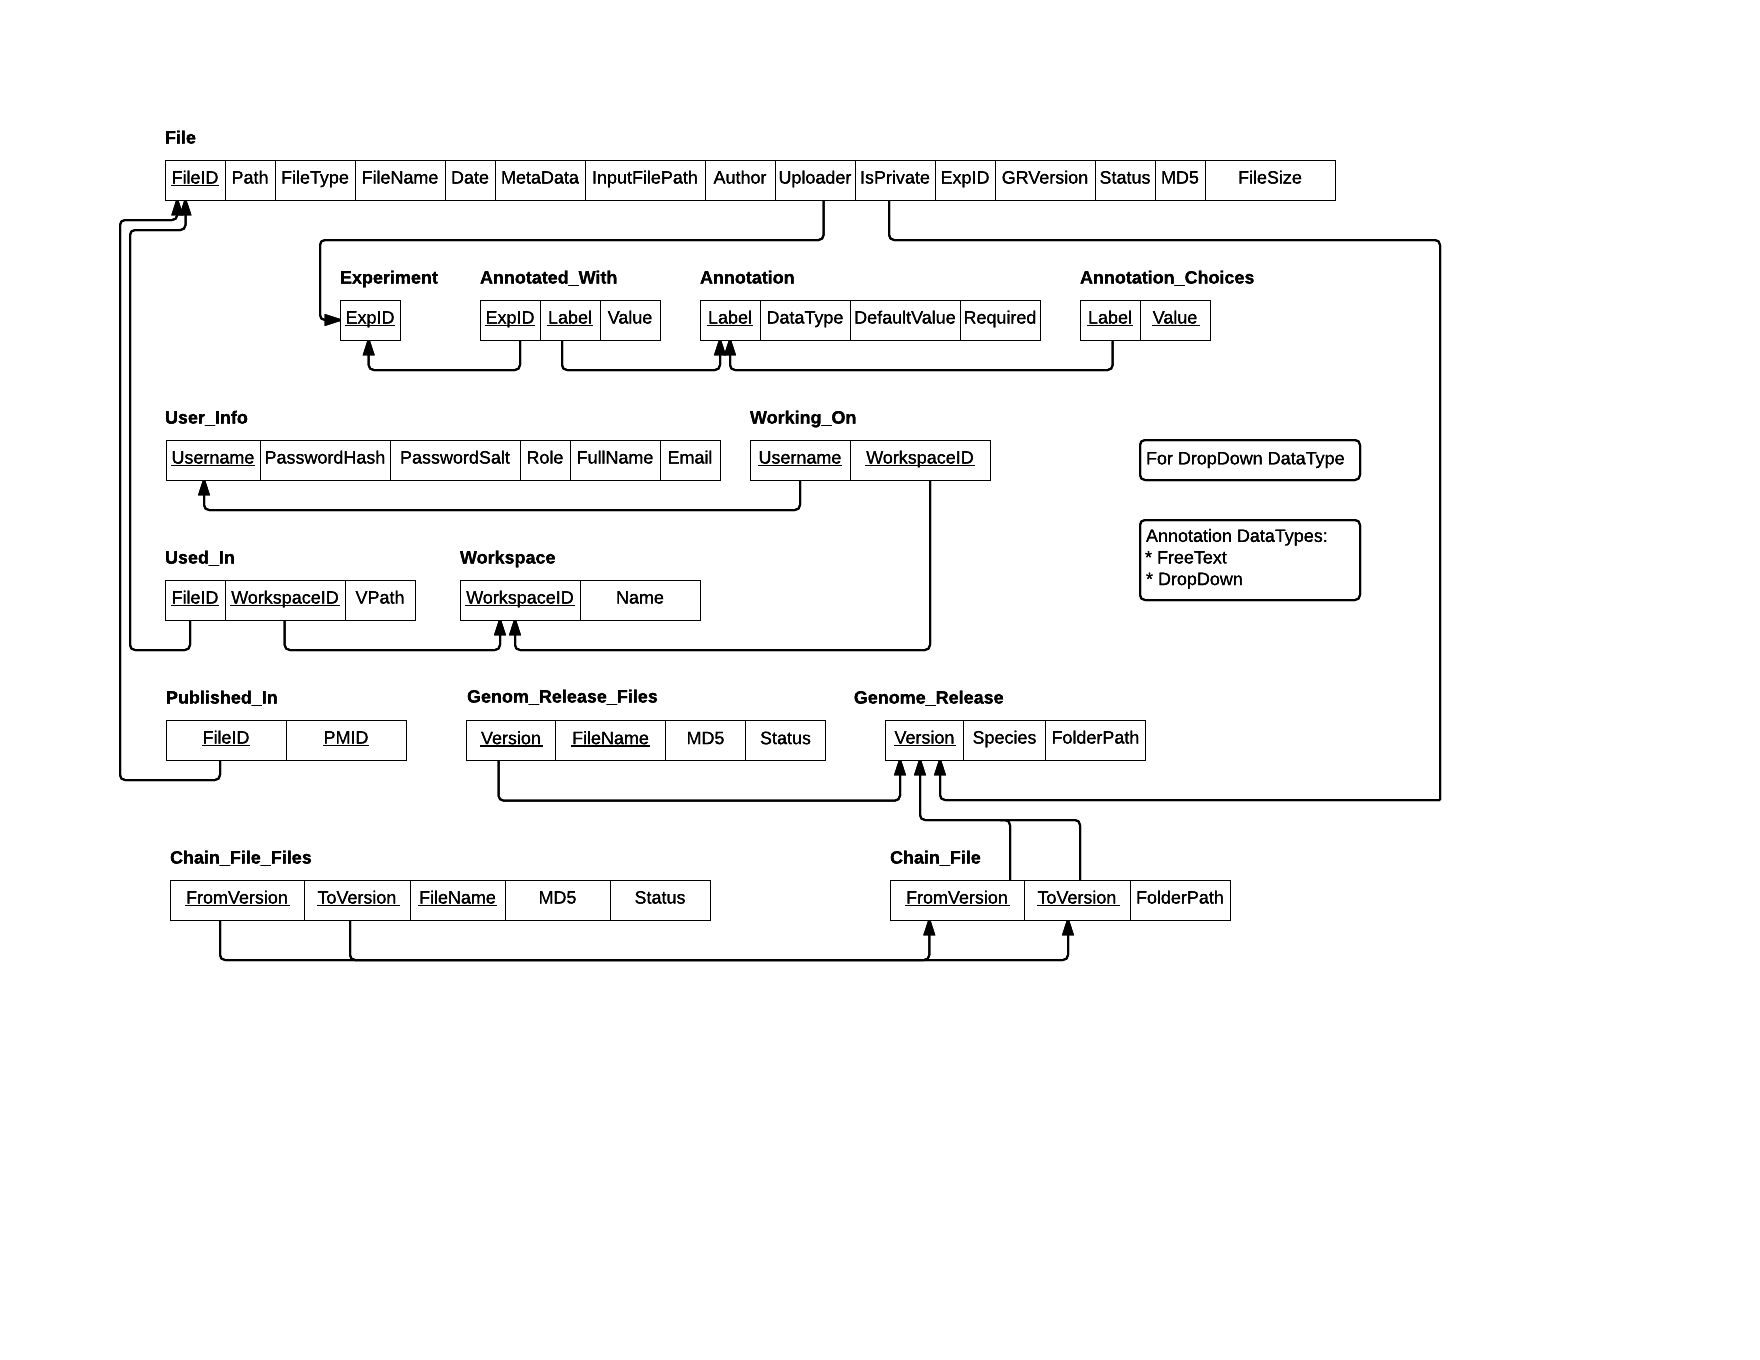
\includegraphics[width=20cm, angle=90, keepaspectratio=true]{dat_database_schema_v3.png}
%\addImageVertical{dat_database_schema_v3.png}
\caption{The database schema}
\label{fig:dat_databaseSchema}
\end{figure}

\FloatBarrier

\subsection{Database Design}
The following section will explain the less obvious columns and their intended use.

\texttt{FileID} is the identification number for a specific file. The data type \texttt{SERIAL} is used and will therefore be auto--generate unique identifiers upon insertion.

\texttt{Path} is the path to the corresponding file in the file system, for example: \\
\texttt{/var/www/data/Experiment1/raw/rawFile1.fastq}

\texttt{MetaData} is the string of parameters used in processing and should be \texttt{NULL} for all raw files.

\texttt{Annotated\_With} is the table that enables the annotation of experiments. The annotation in this table references the \texttt{Annotation}-table, to verify that new annotations are valid.

\begin{example}
To set the Species-annotation to ''Dog'' for the experiment Experiment1, the following tuple would be inserted into the Annotated\_With--table:
  \begin{center}
    \begin{tabular}{| l | l | l |}
      \hline
        \cellcolor{blue!25} ExpID & \cellcolor{blue!25} Label & \cellcolor{blue!25} Value \\
      \hline
      Experiment1 & Species & Dog \\
      \hline
      
    \end{tabular}
  \end{center}
\end{example}

\texttt{Annotation} is the table containing all the possible annotations a user can use to provide extra information about an experiment. This includes the type of annotation which is \term{Drop Down} for annotations where the user can choose from a drop down list, or \term{Free Text} where the user can enter the value freely. There is also support for a default value and annotation forcing where users are forced to provide the information. For \term{Drop Down} annotations the table \texttt{Annotation\_choices} specifies the valid choices.

The \texttt{Genome\_Release} table stores information about the \term{Genome Releases} available for use. This includes the unique version code for a \term{Genome Release}\cite{UCSCGRVERSION}. The \texttt{Genome\_Release\_Files} table stores the information about the files that make up the \term{Genome Release}.

\subsection{The Data Storage Subsystem}
All the classes used in the manipulation of the database and the creation of the file systems directory structure is contained in the java project's \texttt{database} package.

The other \appName\ subsystems execute all updates to the data storage through the \class{DatabaseAccessor} class. As a result there are many methods in this class, however most methods forwards the request to one of the classes in the \texttt{database.subclasses} package. Here the methods that modify the different areas of the data storage system are separated into different classes of more manageable sizes. An UML diagram of the \class{DatabaseAccessor} class and its subclasses is available in \refer{fig:dat_dbac} in  \refer{chap:dat_umls}.

The \class{DatabaseAccessor} utilizes a number of classes in order to return information to the method caller. These classes are contained in the \texttt{database.containers} package and are as follows:
\begin{itemize}
\item \class{Experiment}
\item \class{FileTuple}
\item \class{Annotation}
\item \class{Genome}
\end{itemize}

An UML diagram of these classes is also available in \refer{fig:dat_containers} in \refer{chap:dat_umls}.

\subsection{Interaction}
Below are examples of typical interactions with the \class{DatabaseAccessor} class.

\subsubsection{Adding an experiment}
In order to add an annotated experiment the following steps must be followed:
\begin{enumerate}
\item First the \term{addExperiment} method must be called. This will add one experiment to the database without any annotations set for that experiment. If you try to add one experiment that already exist then the addition will be refused and an exception will be thrown.

\item If there are no annotations that can be used to provide extra information about the experiment they must first be added by calling the \term{addFreeTextAnnotation} or \term{addDropDownAnnotation} methods.

\subitem If a \term{Drop Down} annotation already exists, but there is no suitable choice for the experiment a choice can be added by calling the \term{addDropDownAnnotationValue} method.

\item An available annotation can be used to provide extra information about an experiment by calling the \term{annotateExperiment} method.
\end{enumerate}

Now that an experiment has been added files can be added added to it.

\subsubsection{Annotation Handling}

Annotations can be handled using the methods below.

\begin{tabular}{|l| p{7cm}|}
\hline
\term{getChoices} & gets all the available annotation choices connected to a specific label. For example the possible choices returned for the label "sex" might be "Male, Female and Unknown". \\ \hline

\term{getAnnotations} & returns all annotation labels currently stored in the database. Examples could be "Sex,Species,Tissue,etc.". \\ \hline

\term{getAllAnnotationObjects} & Combines the two previous methods. Here an annotation object is returned that holds all the relevant information including the label, datatype, and the possible choices for a \term{Drop Down} annotation. \\ \hline

\term{changeAnnotationLabel} & updates the given label in the database. This will change the label for all experiments that use it. For example changing "specie" to "Species". \\ \hline

\term{changeAnnotationValue} & updates a value for a specific annotation label. For example changing "Human" to "Homosapien".  \\ \hline

\term{updateExperiment} & Updates an annotation for one specific experiment. Example: "experiment1, Species, Homosapien" can be changed to "experiment1, Species, Fly". \\ \hline

\term{deleteAnnotation} & deletes an unused annotation from the database. This will also delete all the choices for that annotation. \\ \hline

\term{removeAnnotationValue} & removes a single annotation value for a particular label. \\ \hline

\end{tabular}

\subsubsection{File Handling}
The actions of adding and deleting experiment files or genome releases can be performed using the following methods.

\begin{tabular}{|l| p{7cm}|}
\hline
\term{addNewFile} & To add a file you will need to have an experiment added before you call the \term{addNewFile} method. Raw files usually come in pairs and so they can be added together by specifying the input file name. \\ \hline

\term{deleteFile} & Deletes the given file from both the database and the file system. This can be done by either specifying the path or the file's ID number. \\ \hline

\term{addGenomeRelease} & Genome release files must be added one at a time by calling the \term{addGenomeRelease} method. This method returns an upload URL. \\ \hline

\term{removeGenomeRelease} & \term{removeGenomeRelease} removes all the files associated with a genome release. This can only be done if there are no files that have been generated using the specified genome release. \\ \hline
\end{tabular}
\FloatBarrier


\chapter{Implementation}
%This section contains the implementation of the different parts of the system and what tests has been used to ensure its functionality. Directed towards developers. Start with subsubsection here.

This section contains the implementation of the different parts of the system and what tests has been used to ensure its functionality. Here developers can get an understanding of how and why the different parts of the server was completed.

%\section{Clients}

%In this section the implementations of the different clients will be described
%in more detail. The desktop and web clients are explained in the first two
%sections followed by two sections for each of the mobile applications.

\section{Desktop application}
The desktop client is implemented in java 7. The graphical part of the client is made with java swing and the external library swingx. The tree table which is used in the grapical interface is implemented using a modified version of the JxTreeTable found in swingx. The modifications made to the JxTreeTable is that a sorting mechanism has been added and it is possible for the user to choose which columns to show.

The communication with the server is handled with a http protocol involving JSON formatted bodies. The external library GSON and the Apache Http Client are used for the communication.

For dragging and dropping files into the upload tab, the desktop client uses a modified version of the class FileDrop, which was originally written by Robert Harder and Nathan Blomquist and was released as public domain.

\subsection{Testing}

The testing of the system has been quite varied since a large part of the desktop client consists of a graphical interface. The graphical part of the client was tested throughout the developing process and the customers also had a part in testing the interface. Another difficult part of the testing was the communication with the server. A part of it was tested with JUnit tests but the larger part of the testing was made manually by interacting with the GUI and communicating manually with the server.

The client will be involved from an early point since the Scrum developing methodology relies in delivering functionality as early as possible. Because of this, it is given that the system will have bugs, and the client will be of assistance in finding these bugs and reporting them. Before each release of implemented functionality however, they are tested with the Test Cases enclosed to each User Story.

A small number of JUnit tests has been done concerning communication with server API.

\FloatBarrier

\FloatBarrier

\section{Web application}
\subsubsection{Frameworks}
\label{sec:web_frame}
The frameworks used to ease implementing the system. The following frameworks are integrated in the system and the system is built on them. To read more about the frameworks, see the References page.
\paragraph{Backbone}
Backbone\cite{web_1} is a light-weight framework that loosely follows the \textbf{MVC} (model, view, controller) pattern. Out of the \textbf{MVC} components, backbone only has models and views, and the view behaves much like a view and a controller. \textbf{Models} are the parts of code that retrieves and populates data (for example, the model Experiment will obtain and populate the experiments resulting from a search). \textbf{Views} are the HTML representation of models, and they change as models change (When the Experiment model is populated, it is immediately presented on the view that contains that Experiment).
Backbone makes use of \textbf{Events}, where other objects can trigger events and listen to them, which is an effective way to promote decoupling between components. It also uses \textbf{Collections}, that are ordered sets of models. A collection will automatically be provided with underscore array and collection methods for convenient set manipulations (You can, for example loop through a collection with .each() instead of writing a for-loop). We chose to use backbone because we wanted more structure in our web application. With more structure, it is easier to collaborate as we can divide up the work - keeping our JavaScript in various model, collection and view files.

\paragraph{Bootstrap}
Bootstrap\cite{web_2} is a front-end framework that contains HTML and CSS-based design templates for typography, buttons, forms, navigations, and the like. Instead of creating our own buttons, deciding on colors, how big they are, and micro-managing how they fit with everything else on the page, we can use bootstraps templates that handles all of that for us, leaving us able to focus on architecture. We chose to use it to save time on development and make the look of our web app easily customizable.
\paragraph{AJAX}
AJAX\cite{web_3} stands for \textbf{Asynchronous JavaScript and XML}. It is a technique for creating fast and dynamic web pages. Despite the name, the use of XML is not required; JSON is often used instead, as we have done in our web app. AJAX allows web pages to be updated asynchronously by exchanging small amounts of data with the server, so that you only update parts of a web page without having to reload the entire page (like websites that don’t use AJAX has to). For example, when “search” is clicked in our navigation bar, only the bottom half of the website is being updated, and displaying the search view. The navigation bar does not have to be reloaded, but remains as is on top.

\paragraph{JSON}
JSON\cite{web_4} is short for \textbf{JavaScript Object Notation} and is a format that is primary used to transmit data between a server and web application instead of using XML or other formats.
JSON is formatted as text which is easy to read consisting of attribute-value pairs.
JSON was used in this application because JSON uses the same syntax as JavaScript and therefore we do not need to make our own parser as we would have to do for e.g. XML. JSON does also work very well together with Backbone as it has integrated methods using the JSON format.

\paragraph{RequireJS}
RequireJS\cite{web_5} is a file and module loader for JavaScript. RequireJS lets files require other files much like \texttt{\#include} in Java this is very handy for the programmer. It is used because it helps to structure the application.
\paragraph{JQuery}
The purpose of JQuery\cite{web_6} is to make it easier to use JavaScript on a website. It takes a lot of common tasks that require many lines of JavaScript code to accomplish, and wraps them into methods that you can call with a single line of code. It simplifies other things as well, like AJAX calls and DOM manipulation, both of which are in frequent use in our web application.
\subsubsection{Testing frameworks}
For testing we have used three libraries to make testing easier: chai, mocha and sinon. Together they let us make a page for testing where all tests and results will be shown visually.
These libraries or testing frameworks will be discussed below.
\paragraph{Chai \& Mocha}
Mocha\cite{web_8} is a test framework while Chai\cite{web_7} is an expectation framework. While Mocha setups and describes test suites, Chai provides convenient helpers to perform all kinds of assertions against JavaScript code. We use these frameworks to do unit testing on our models and collections.

\paragraph{Sinon}
Sinon\cite{web_9} is a framework used to \textit{“fake environment”}. When doing unit testing, we don’t want to depend on things that are external to the unit of code that we are testing. We can use Sinon for stubbing and mocking external dependencies and to keep control on side effects against them. For example, we can use Sinon to create spies to see if an event has been triggered, and to create fake servers that respond with fake pre-planned responses to our queries.
\subsubsection{Our Tests}
We have performed unit tests on our model and collection files, all of which can be found in our root folder under \filePath{/tests/}, more specifically \filePath{genomizer-web/tests/}. To see the tests, simply open the index.html in a web browser, and they will run.

\FloatBarrier

\section{Android application}
The Android application has been implemented with \verb!Java!, the default language for developing Android applications. The framework is called Android Application Framework and consist of view managers, resources and more. The application is developed for devices with, reaching over 90\% of all devices (May 2015).
\subsection{Environment}
		The application has been developed in Eclipse suited with Android Software Development Kit (SDK). The SDK consist of debuggers, libraries etc.
\subsection{Emulation}
		The application has been emulated on and Android Virtual Device (AVD). This emulator comes bundled with the SDK and is a great tool simplifying Android development.
\subsection{Android Support Library}
		The Android Support Library has been used in order to enable functionality introduced in later API levels to earlier API levels.
\subsection{Technologies}
	The communication with the server is done by \verb!HTTP! and \verb!REST!, exchanging \verb!JSON!-packages.
\subsection{Testing}
	The model classes of the application has been tested with \verb!JUnit 3!. Since the application is so heavy on graphical interaction (wich is hard to test) a lot of manual testing has been done, both on AVD and on real hardware devices. The acceptance tests that is stated in \refer{tests} and applicable to a mobile application have all been satisfied.


\FloatBarrier

\section{iOS application}
The iOS application has been implemented using Objective C. The decision to use Objective C was made largely because it is the standard language used for writing iOS applications. 
In the following sections, details regarding the implementation of the iOS application are described using sequence diagrams. The section ends with a description of testing strategies.

\subsection{Login}

When the user tries to log in to the system, they enter username and password and clicks on the login button. The username and password is sent to the server which validates that they are valid. If they are valid, the user is presented with the main view of the application, otherwise an error message is displayed. This sequence is shown in  \refer{fig:ios_sequence_login}.

\begin{figure}[ht]
\addImageVertical{ios_sequence_login.png}
\caption{Login sequence diagram.}
\label{fig:ios_sequence_login}
\end{figure}

\subsection{Search}

Once the user is logged in to the system and they have reached the main view, they can immediately start searching by selecting a number of search criteria on the screen and pressing the search button. The search criteria are converted into a valid \term{PubMed}-style query which in turn is converted into a valid \term{HTTP request} and sent to the server. The server responds with all results matching the search criteria and the results are presented to the user in a \term{SearchResultView}. This sequence is shown in \refer{fig:ios_sequence_search}.

\begin{figure}[ht]
\addImageVertical{ios_search_sequence_diagram.png}
\caption{Search sequence diagram.}
\label{fig:ios_sequence_search}
\end{figure}

\subsection{Experiment Selection}

In the \term{SearchResultTableView}, the user can click on an experiment to see which files are contained in an experiment. The file contents of an experiment is displayed in a \term{FileView}. The sequence is shown in \refer{fig:ios_sequence_experiment_selection} 

\begin{figure}[ht]
\addScaledImageVertical{0.5}{ios_select_experiment_sequence_diagram.png}
\caption{Experiment selection sequence diagram.}
\label{fig:ios_sequence_experiment_selection}
\end{figure}

\subsection{File Selection}

From the \term{FileView}, the user can select any number of files to add to a list of currently selected files by pressing the switch button next to each file name and pressing the \term{Add to Selected files} button. After that, the user can press the \term{Selected Files} button to go to the \term{Selected Files View}. This sequence is shown in \refer{fig:ios_sequence_file_selection}

\begin{figure}[ht]
\addScaledImageVertical{0.5}{ios_select_file_sequence_diagram.png}
\caption{File selection sequence diagram.}
\label{fig:ios_sequence_file_selection}
\end{figure}

\subsection{Convert Request}

As seen in \refer{fig:ios_sequence_convert_request2}, convert requests are sent with very few steps. 

\begin{figure}[ht]
\addScaledImageVertical{0.5}{ios_send_convert_sequence_diagram.png}
\caption{Send convert request.}
\label{fig:ios_sequence_convert_request2}
\end{figure}
\FloatBarrier

\subsubsection{Segue Control}
A segue control package has been implemented to avoid multiple segues being executed at the same time. When a segue is started, a static \term{BOOL} is set to \term{YES} in XYZSegueController. When the segue is finished, the \term{BOOL} in XYZSegueController is set to \term{NO}. This means that the \term{BOOL} is \term{YES} when a segue is being executed, and \term{NO} otherwise. Every time a segue is going to be executed, it first checks the value of the \term{BOOL}. If a segue is already being executed, i.e. the \term{BOOL} is \term{YES}, the new segue is aborted.

\subsection{Testing}

We have worked using the principles of TDD, which means that Unit-tests have been written for nearly all underlying classes. This includes JSONBuilder, ExperimentDescriber, Experiment, ExperimentFile, and ExperimentParser. These tests check all required functionality, including but not limited to proper object creation. Exactly what all the tests do is explained in the test names and comments. ServerConnection has not been tested, this is work for next years workers. User interface functionality and integration testing has been done using exploratory methods. Some UI functionality has been tested using automated tests, where we recorded a certain combination of clicks, and let the computer do them instead. 

\FloatBarrier

\section{Server}

In this section the server and its different subsystem are displayed.
Information about how the software design was realised in code will be provided.

\subsection{Communication}
This section explains implementation details of certain bits of the communication/control part of the system.
\subsubsection{Doorman}
The doorman is a class which handles all incoming connections and requests. The doorman reads the header and checks what kind of HTTP method it is (GET, PUT, PUSH, PULL or DELETE). A switch statement switch on these different methods.\\
\\
After switching on the different methods another switch statement is used to switch on the different types of commands, for example /experiment, /file, /search or /process. From that point a specific command object is created corresponding to the correct command, for example \textbf{GET /experiment} will create a \term{getExperimentCommand}.
\subsubsection{Authorization}
The communication between a client and the server is authorized by a user-unique token which is created when the user sends a login request. A token is created when a user has logged in successfully and the token is sent back to the user so that the user can thereafter use this in future requests. 
\begin{figure}[h]
\addImage{com_authorization.png}
\caption{1. The user sends a login request without any authorization token. 2. The server checks the given password. 3. The server creates a unique token for the user. 4. Server sends the token back to the user in a response. 5. Now that the user has a unique token, the token is placed in the header whenever the user sends another request.}
\label{fig:com_authorization}
\end{figure}
The token created when a user sends a login is stored in the server memory until the user sends a logout request.
\subsubsection{Removing inactive tokens}
The server has a function which removes inactive tokens after a set limit of time. This is done because a client sometimes skips sending a logout request when shutting down the client program. The InactiveUuidsRemover class is used to achieve this goal. In a thread it sleeps for one hour before checking all clients. If any client hasn't sent a request for 24 hours, the client token is removed from the server memory. 
\\
This feature may be turned of with the flag "-nri".
\subsubsection{Command object}
The command object represent a specific command. It is created from the RESTful header and/or the JSON body sent from the client. The JSON API provides methods for automatic parsing of the JSON body into an object. The fields in the command object created must match the attributes in the JSON body. This match is case sensitive
\paragraph{Execute}
Every command object must implement a execute method. This method is the part of the command which uses the system interface to perform the task that corresponds to the command.\\
\\
The execute method returns a response object which is sent up to the doorman which then sends the response to the client. 
\paragraph{Validation}
Every command must implement a validate method. This method is run after the command is created but before the command is executed.\\
\\
The validate method returns a boolean. If the command is correctly parsed with correct data the method returns true, otherwise false. This validate is used to prevent unnecessary communication.
\subsubsection{Heavy work thread}
For heavy work a queue, namely work handler is used. The command which is put in this queue is ProcessCommand. All the command objects which is in the queue, are executed one at a time  in the order first in first out. This execution is done by another thread with the only responsibility to do this kind of heavy work. The thread constantly checks whether the queue is empty or not and if there is a command object in the queue the thread polls the command object and executes it.\\
\\
Which command that is put in the queue or not is determined in the method processNewCommand  in the class CommandHandler. 
\subsubsection{Response object}
There are different response objects for different kind of responses since the form of the response to the client depends on the command the client initially sent.\\
\\
The response object contains all the data necessary to create a RESTful header and a JSON body for the response.
\subsubsection{Testing}
Testing has been done in multiple steps. The first step is unit testing, where individual methods are tested. This is often difficult
due to the fact that the responsibility of handling client requests is shared by multiple classes. To catch these test cases a client
dummy has been frequently used, which is the next step. 
It simulates a client by sending HTTP requests and examines the response from the server. It is used
manually to test a particular use case, and to see that the server behaves as intended for that request.
After a feature has passed the client dummy it is pushed to a test server, where it is open for other clients to test and debug.
If no bugs are found the feature is declared complete and can be released.

\FloatBarrier

\subsection{Conversion}

\subsection{SmoothingAndStep}

The basic algorithm is a dynamic arrayList which carries the rows that are relevant at a given time, smoothing on the first row is performed. The newly smoothed value is shifted out and replaced with a fresh row. This becomes a dynamic window that traverses the entire file one row at a time.

\subsubsection{Methods}

\begin{itemize} 
\item smoothing : The one public method of the class. It controls the whole process and calls the other methods. It takes in the following parameters:
\begin{itemize}
\item int[ ] params: An array with 5 integers representing parameters.
     params[0]: Window Size, the nu 
mber of signal values that the smoothing
      		  should be calculated on. \newline
      params[1]: Wether the smoothing should be trimmed mean (0) or median (1)\newline
      params[2]: Minimum numbers to smooth. A number that says how many signal
      		  values the program at least need in order to smooth one row.
      		  This number must be smaller than windowSize. \newline
      params[3]: Can either be 1 or 0. If 1 the program will calculate the
      		  total mean value for all rows and print those. \newline
      params[4]: Print zeroes. If the program should print rows where the
      		  signal value is 0 the flag should be (1), if (0) the program
      		  will not print the zeroes. \newline
\item String inPath: A filepath to the source file.
\item String outPath: A filepath to either an existing file to be overwritten or of a location and name that will become the path to a newly created file.
\item int stepSize:  An integer larger than 0 that tells if there should be stepping. No stepping will be done if the number is 1.
\end{itemize}

The method will also return the total mean of every row in the file if that flag is set properly.

\item smoothOneRow: Checks wether smoothing should be trimmed mean or median and calls the corresponding method, after this is done it calls the method that writes to the new file.

\item smoothTrimmedMean: Extracts the first position from the data array and initiates it's value to min and max values. We do this because trimmed mean means that we should remove the largest and smallest number from the mean value in order to get a more reliable/stable result. We then check that we have more numbers in the data array than the minimum numbers to smooth number. In order to avoid doing unnecessary calculations. 

\item smoothMedian: This method tries to fill an array with window size number of signal values and then pass this array to a method that finds which number is the median.

\item writeToFile: This method does three different things. It check wether we should print zeroes in the outfile. It also check wether the current position is divisible with stepSize to determine if the row should be written to the outfile or skipped.  After these two checks it either writes the row to the new file or not.

It also check wether we want to print the total mean of the whole file and/or if we should then it counts up the proper variables.

\item shiftLeft: Removes the first row from the data array and adds one row to the end of it.  It then checks wether the new row is of a different chromosome than the others, if so it calls the special method chromosomeChange.

\item chromosomeChange: This method knows that the last element in the data array is a new chromosome. It then reads and smooths as many rows as it can before hitting the cutoff number (minimum number of rows to smooth). It then writes and removes these values from the data array aswell. It's important to note that so far it doesn't add new values to the array. Afterwards the method tries to refill the array with the new chromosome until it has window size number of rows.



\end{itemize}



 
\FloatBarrier

%\subsection{System administration}
%\FloatBarrier

\subsection{File-transfer}
To handle all the downloads and uploads to and from the clients, two php-scripts have been written. 

Both scripts uses the token provided by the client to authenticate the user. This token is sent to the server which will send a code back to the script. The code will be '200' if the client has provided a valid token, and '401' if the token is invalid. The upload script gets the token in an 'Authorization' header, while the download script gets the token in an 'Authorization' header from the desktop client and in an 'Authorization' parameter from the web client.

When the client downloads or uploads a file it will send a path to the script in a 'path' parameter. This path will then be validated against the database. For downloading it will check if the file is 'Done' and when uploading that the file is not 'Done'.

When an upload has been finished and validated the script will change the status for this file to done and then send a '201' response code to the client. When a download request has been validated the script will send the file as an octet-stream as a response to the client.

\FloatBarrier

\subsection{Data Storage}
\section{Implementation}
The following text describes the different classes the server uses to cummunicate with the database.
\subsection{Annotation}
When a user wants the properties of an \term{annotation} they will retrieve this object. It holds information about the data type, label, forced annotation, default value and annotation choices for drop down menus. With this object the graphical interfaces can set up a search view dynamically.

\subsection{Experiment}
A container of an experiments annotations and their values. The annotation labels and values are contained in a \term{hashmap} with label as key. All files corresponding to the actual experiment lies in a list of \term{FileTuple} objects.

\subsection{FileTuple}
A simple class that holds all information of a file in variables found in the database. Holds links for download and upload of the specific file.

\subsection{FilePathGenerator}
When a user wants to write or download a file, the \term{FilePathGenerator} class will take care of giving the server a file path. When a new experiment is added to the database, FPG is called and it will create a folder for the experiment and sub folders for the different file types. When a new \term{genome version} is to be added to the database, FPG will create file paths to a folder outside of the experiment folders. They are divided into folders corresponding to species.  This is done to give access to genome files independent of experiment id's. Chain files are given paths to sub folders within the species folders in the genome root folder.

\subsection{PubMedToSQLConverter}
Converts a string with \term{pubMed} notations and returns an \term{SQL query}. PubMed searches can take this shape: \texttt{raw1[FileType] AND Per[Author]} which means \term{search for all raw files that Per created}. The user enters the values with variables in a logical sequence and can add parentheses for further filtering. \term{AND}, \term{OR} and \term{NOT} are commands that can be used in the sequence. The converter can both be used for file- and experiment searches. All the variables in the pubMed string are converted to the \texttt{WHERE} section of an SQL query. When a method is called in the database API (DatabaseAccessor), the first half of the query will be combined with the one generated by the converter to form a full query. Depending on which method is called in the \term{API} (what the user wants to do), the first half of the query will vary.

\subsection{DatabaseAccessor}
A class that serves as API for the server for database access. It handles all connections and queries to the database. The methods simplifies queries to the database by taking as few parameters as possible to accomplish a sufficient database search. The returns of the different methods are made as simple as possible depending on the amount of data generated. If only one column is to be returned after a search, a list is sufficient. When a user wants information on several files, lists of objects will be returned with all data. \term{Prepared Statements} are created from a combination of queries and variables to avoid SQL injections. Methods that have some resemblance are grouped together for easier navigation in the API. The class itself generates no database queries. This is done in other smaller classes divided into different types of tasks. The class is large and can't be shortened since it's the API front to the database.

\section{Testing}
All methods are created with \term{Test Driven Development} (TDD). Testing is done before implementation. The better part of the testing is creating queries that gives the right results. All queries have at at least one test to verify it's functionality. The tests are run in a test suite so every method in the whole program can be tested in one run. Database methods have setup and teardown methods for setting up and resetting the database between the different tests. This is done to prevent a test to influence the result of another test. Stress tests are also implemented with the goal to determine functionality by simulating multiple users working in parallel.
\FloatBarrier


\chapter{Testing}
\input{testing/testing.tex}

\chapter{Limitations}
\section{Clients}
\subsection{Desktop}
\FloatBarrier
\subsection{Web}
\subsection{Moving backwards in the browser does not hide modal windows}
When navigating to a modal window the URL is updated, and added to the browser history. When using the browser back-button the modal is not closed, but the URL is still updated. \\
\\
 Modify ModalAC and the router
\subsection{Error handling when uploading experiments}
If there is an error when adding files to an experiment the experiment collapses so the user won't get a chance to correct it's mistake \\
\\
Start uploads of files when all files have been added without errors. 
\subsection{Old authorization token causes page redirect}
If the authorization token expires the user will be sent to the login screen and any input entered will dissapear. \\
\\
Show login modal without redirecting to root url and save errorous ajax-request and resend it when the login has been completed.
\subsection{Code duplication in SearchResults and Experiments}
The collections SearchResults and Experiments represents the same models. But are different collections as they have different URL. It might be better to have the both use the same collection. \\
\\
Merge SearchResults and Experiments one collection.
\subsection{No warning when closing tab during upload.}
If a upload is in progress, there is no warning when closing the tab and the upload is canceled directly. \\
\\
There are some code for this in view/Upload.js, but it's currently broken.

\FloatBarrier
\subsection{Android}




\begin{thebibliography}{10}
\bibitem{BOWTIE}
  Langmead, Ben and Trapnell, Cole and Pop, Mihai and Salzberg, Steven L and others,
  \emph{Ultrafast and memory-efficient alignment of short DNA sequences to the human genome}.
  Genome Biol 10(3),
  2009.

\bibitem{LIFTOVER}
  LiftOver: \url{http://genome.sph.umich.edu/wiki/LiftOver} Retrieved 30/5 -14

\bibitem{IGB}
  Integrated Genome Browser: \url{http://bioviz.org/igb/} Retrieved 31/5 -14
\bibitem{des_1} \textit{technoweenie}. ''Release Your Software''.
\textit{GitHub}. July 2, 2013. Web. May 29, 2014. <\url{https://github.com/blog/1547-release-your-software}>

\bibitem{des_2} Preston-Werner, Tom.  ''Semantic Versioning 2.0.0''. Web.
May 29, 2014. <\url{http://semver.org/}>

\bibitem{des_3} \textit{National Center for Biotechnology
Information}.  ''PubMed Advanced Search Builder''. \textit{U.S. National Library
of Medicine}. October 28, 2009. Web. May 29, 2014. <\url{http://www.ncbi.nlm.nih.gov/pubmed/advanced}>

\bibitem{exp_apache2user} Authentication and Authorization \\
\url{http://httpd.apache.org/docs/2.2/howto/auth.html}\\
Retreived 8/5- 2014
\bibitem{exp_gitguide} git - the simple guide \\
\url{http://rogerdudler.github.io/git-guide/}\\
Retreived 8/5- 2014
\bibitem{exp_gitguide2} Git for beginners: The definitive practical guide \\
\url{http://stackoverflow.com/questions/315911/git-for-beginners-the-definitive-practical-guide}\\
Retreived 8/5- 2014
\bibitem{exp_sshguide} How to generating SSH Keys\\
\url{https://help.github.com/articles/generating-ssh-keys}\\
Retreived 8/5- 2014

\bibitem{web_1} ''Backbone.js documentation''. Web. May 29, 2014. <\url{http://backbonejs.org/}>
\bibitem{web_2} Otto, Mark. ''Bootstrap documentation''. Web. May 29, 2014. <\url{http://getbootstrap.com/}> 
\bibitem{web_3} ''AJAX (programming)''. \textit{Wikipedia}. Web. May 29, 2014. <\url{http://en.wikipedia.org/wiki/Ajax_(programming)}> 
\bibitem{web_4} ''JSON''. \textit{Wikipedia}. Web. May 29, 2014. <\url{ http://en.wikipedia.org/wiki/JSON}> 
\bibitem{web_5} ''RequireJS documentation''. Web. May 29, 2014. <\url{http://requirejs.org/}>
\bibitem{web_6} ''JQuery documentation''. Web. May 29, 2014. <\url{http://jquery.com/}>
\bibitem{web_7} ''Chai documentation''. Web. May 29, 2014. <\url{http://chaijs.com/}>
\bibitem{web_8} Holowaychuk, TJ. ''Mocha documentation''. Web. May 29, 2014. <\url{http://visionmedia.github.io/mocha/}> 
\bibitem{web_9} Johansen, Christian. ''Sinon documentation''. Web. May 29, 2014. <\url{http://sinonjs.org/}>

\end{thebibliography}

\begin{appendix}

\chapter{\textit{User Stories}}
\label{chap:userstories}

A \term{User Story} is a description of functionality in non technical terms. It describes the wishes of a certain user group and a motivation for why the function is needed.

\section{Implemented user stories}
\begin{figure}[h!]
\userstory{Annotation}{To structure the data files \\ the researchers \\ want to be able to annotate the data files.}
\caption{Annotation user story}
\label{us:annotation}
\end{figure}

\begin{figure}[h!]
\userstory{Single download}{To scrutinize a single data file \\ the researchers \\ want to be able to download a specific file.}
\caption{Download user story}
\label{us:singleDownload}
\end{figure}

\begin{figure}[h!]
\userstory{Single upload}{To store a single data file \\ the researchers \\ want to be able to upload a specific file.}
\caption{Upload user story}
\label{us:singleUpload}
\end{figure}

\begin{figure}[h!]
\userstory{Search for data}{To analyse data \\ the researchers \\ want to be able to search for specific types of data.}
\caption{Search for data user story}
\label{us:searchData}
\end{figure}

\begin{figure}[h!]
\userstory{Raw to profile}{To be able to analyse \\ the researchers \\ want to process raw data to profile data (using bowie and then Philge’s code).}
\caption{Raw to profile user story}
\label{us:rawToProfile}
\end{figure}

\begin{figure}[h!]
\userstory{Delete data}{To save space \\ the researchers \\ want to be able to delete data from the database.}
\caption{Delete data user story}
\label{us:deleteDate}
\end{figure}

\begin{figure}[h!]
\userstory{Change annotation}{To correct and update annotations \\ the researchers \\ want to be able to change data annotations.}
\caption{Change annotation user story}
\label{us:changeAnnotation}
\end{figure}

\begin{figure}[h!]
\userstory{Backup}{To prevent loss of data \\ the researchers \\ want the data to be backed up.}
\caption{Backup user story}
\label{us:backup}
\end{figure}

\begin{figure}[h!]
\userstory{Password protected}{To protect the database from unauthorized use \\ the researchers \\ want the application to be password protected.}
\caption{Password protected user story}
\label{us:passwordProtected}
\end{figure}

\begin{figure}[h!]
\userstory{Add genome release / reference genome}{To be able to annotate the data properly and extract genome reference \\ the researchers \\ want to be able to add genome releases and reference genome.}
\caption{Add genome release / reference genome user story}
\label{us:addGenomeRelease/referenceGenome}
\end{figure}

\begin{figure}[h!]
\userstory{Batch download}{To scrutinize several data files \\ the researchers \\ want to be able to download multiple files at once.}
\caption{Batch download user story}
\label{us:batchDownload}
\end{figure}

\begin{figure}[h!]
\userstory{Convert common file formats}{To get data in a certain convenient file format \\ the researchers \\ want to convert between common file formats (WIG, SGR, GFF3, BED).}
\caption{Convert common file formats user story}
\label{us:convertCommonFileFormats}
\end{figure}

\begin{figure}[h!]
\userstory{Work queue}{To reduce server load \\ the researchers \\ want to queue time consuming work.}
\caption{Work queue user story}
\label{us:workQueue}
\end{figure}

\begin{figure}[h!]
\userstory{User rights}{To allow invitation of guests (postgraduate students or other researchers etc.) \\ the researchers \\ what to have different users types with different rights.}
\caption{User rights user story}
\label{us:userRights}
\end{figure}

\begin{figure}[h!]
\userstory{Batch upload}{To analyse, share and have greater access to data \\ the researchers \\ want to be able to upload multiple files and batch annotate them to a shared location.}
\caption{Batch upload user story}
\label{us:batchUpload}
\end{figure}

\begin{figure}[h!]
\userstory{Sort search results}{To easier find specific result \\ the researchers \\ want to filter the search result.}
\caption{Sort search results user story}
\label{us:sortSearchresults}
\end{figure}

\section{Product backlog}

\begin{figure}[h!]
\userstory{Add chain file}{To be able to convert between genome releases \\ the researchers \\ want to upload chain files (LiftOver).}
\caption{Add chain file user story}
\label{us:addChainFile}
\end{figure}

\begin{figure}[h!]
\userstory{File traceabillity}{To be able to access the underlying raw data or profile data \\ the researchers \\ want the raw data files to be traceable from profile files and the profile files to be traceable from the region data (if available) when the files have been generated on the server.}
\caption{File traceabillity user story}
\label{us:fileTraceability}
\end{figure}

\begin{figure}[h!]
\userstory{Convert genome release}{To easier handle files \\ the researchers \\ want to convert files between genome releases (LiftOver).}
\caption{Convert genome release user story}
\label{us:convertGenomeRelease}
\end{figure}

\begin{figure}[h!]
\userstory{Extract genome reference sequence}{To analyse the reference genome \\ the researchers \\ want extract the reference genome sequence for a given region data.}
\caption{Extract genome reference sequence user story}
\label{us:extractGenomeReferenceSequence}
\end{figure}

\begin{figure}[h!]
\userstory{Advanced batch upload}{To simplify mass upload ~500 files \\ the researchers \\ want to batch annotate files to be uploaded in a spreadsheet.}
\caption{Advanced batch upload user story}
\label{us:advancedBatchUpload}
\end{figure}

\begin{figure}[h!]
\userstory{Profile to region}{To be able to find regions of interest \\ the researchers \\ want to process profile data to region data (Per’s code).}
\caption{Profile to region user story}
\label{us:profileToRegion}
\end{figure}

\begin{figure}[h!]
\userstory{Workspace}{To be able to save work in a convenient way \\ the researchers \\  want to have some sort of workspace view where all kind of results/data can be saved.}
\caption{Workspace user story}
\label{us:workspace}
\end{figure}

\begin{figure}[h!]
\userstory{Unread results}{To avoid missing results \\ the researchers \\  want to see which results are unread.}  \caption{Unread results user story}
\label{us:unreadResults}
\end{figure}

\begin{figure}[h!]
\userstory{Preview of file}{To correctly annotatate a file \\ the researchers \\ want to preview a portion of a file.}
\caption{Preview of file user story}
\label{us:previewOfFile}
\end{figure}

\begin{figure}[h!]
\userstory{Work scheduling}{To strategically spread the servers workload over time \\ the researchers \\ want to be able to schedule the processing/analysis of data.}
\caption{Work scheduling user story}
\label{us:workScheduling}
\end{figure}

\begin{figure}[h!]
\userstory{Time estimation}{To warn for time consuming jobs \\ the researchers \\ want to have a time estimation for jobs.}
\caption{Time estimation user story}
\label{us:timeEstimation}
\end{figure}

\begin{figure}[h!]
\userstory{Plot overlap analysis}{To see region overlap of genomes \\ the researchers \\ want to plot an overlap analysis (see separate user story).}
\caption{Plot overlap analysis user story}
\label{us:plotOverlapAnalysis}
\end{figure}

\begin{figure}[h!]
\userstory{Plot average regions}{To view data \\ the researchers \\ want to plot average of regions with the profile data.}
\caption{Plot average regions user story}
\label{us:plotAvarageRegions}
\end{figure}

\begin{figure}[h!]
\userstory{IGB Session}{To be able to make IGB analysis \\ the researchers \\ want to retrieve a IGB session file.}
\caption{IGB Session user story}
\label{us:IGBSession}
\end{figure}

\begin{figure}[h!]
\userstory{Combine regions}{To find interesting regions \\ the researches \\ want to select multiple files and combine their regions (union, intersect).}
\caption{Combine regions user story}
\label{us:combineRegions}
\end{figure}

\begin{figure}[h!]
\userstory{Create region subset}{To retrieve certain parts of regions \\ the researchers \\ want to create region subsets using reference points.}
\caption{Create region subset user story}
\label{us:createRegionSubset}
\end{figure}

\begin{figure}[h!]
\userstory{Calculate average of region}{To find the average protein binding value for a region \\ the researchers \\ want to calculate average of regions with the profile data. (Possibly split into a number of bins).}
\caption{Calculate average of region user story}
\label{us:calculateAverageOfRegion}
\end{figure}

\begin{figure}[h!]
\userstory{Overlap analysis}{To conduct overlap analysis \\ the researchers \\ want to divide regions bins, either by value or by order.}
\caption{Overlap analysis user story}
\label{us:overlapAnalysis}
\end{figure}

\begin{figure}[h!]
\userstory{Save analysis results}{To be able to return to previous work \\ the researchers \\ want to save analysis results(in workspace).}
\caption{Save analysis results user story}
\label{us:saveAnalysisResults}
\end{figure}


\chapter{Android application: \term{UML}-diagrams}
\label{chap:and_appendix}

In this appendix the \term{UML}-Class-diagrams of the Android application will be
presented. 

\begin{figure}[h]
    \addImage{and_UML_model_sprint2.jpg}
    \caption{Android UML of model}
    \label{fig:and_umlmodel}
\end{figure}  
\begin{figure}[h]	
    \addImageVertical{and_UML_android_sprint2.jpg}
    \caption{Android UML without model}
    \label{fig:and_uml}
\end{figure}  
\FloatBarrier



\chapter{Desktop application: \term{UML}-diagrams}
\label{chap:des_appendix}
%\input{appendices/des_appendix}

\chapter{Data Storage: \term{UML}-diagrams}
\label{chap:dat_umls}
\begin{figure}[!ht]
\addScaledImage{0.45}{dat_dbac.png}
\caption{\texttt{DatabaseAccessor} and its subclasses}
\label{fig:dat_dbac}
\end{figure}

\begin{figure}[!ht]
\addImage{dat_containers.png}
\caption{The container classes used to return information}
\label{fig:dat_containers}
\end{figure}

\chapter{Server API}
\section{API}

\subsection*{Connection}
Login/Logout to and from the server. When a user has been verified a token (user-id) is supplied in the response. The token is generated from the current date and the users password. It is then hashed and given an expiration date. The token should be supplied in the Authorization header for each request in order to identify the user.

\subsubsection*{\textbackslash login}
\begin{verbatim}
Login to the server [POST]
+ Request (application/json)

        {
         "username": "uname", 
         "password": "pw"
        }

+ Response 200 (application/json)
    
            {
             "token": "user-id"
            }

Logout from the server [DELETE]
+ Request

    + Header
    
            authorization: user-id
        
+ Response 200
\end{verbatim}
\newpage
\subsection*{Experiment}
\begin{verbatim}
An experiment containing annotations and files. `experiment-id` in the header of the 
request is the unique id (name) of the experiment.

+ Parameters
    + name ... Name and id of the experiment
    + created by ... Which user created the experiment
    + annotations 
        + pubmedId
        + type
        + specie
        + genoRelease
        + cellLine
        + devStage
        + sex
        + tissue
        + ...
\end{verbatim}            

\subsubsection*{\textbackslash experiment} 
\begin{verbatim}
### Add an Experiment [POST]
+ Request (application/json)

    + Headers
    
                Authorization: token
                
    + Body 
    
            {
                "name": "experimentId",
                "createdBy": "user",
                "annotations": 
                             [
                             {
                              "name": "pubmedId",
                              "value": "abc123"
                             }, 
                             {
                              "name": "type",
                              "value": "raw"
                             },
                             {
                              "name": "specie",
                              "value": "human"
                             },
                             {
                              "name": "genome release",
                              "value": "v.123"
                             },
                             {
                              "name": "cell line",
                              "value": "yes"
                             },
                             {
                              "name": "development stage",
                              "value": "larva"
                             },
                             {
                              "name": "sex",
                              "value": "male"
                             },
                             {
                              "name": "tissue",
                              "value": "eye"
                             }
                             ]
                
            }
        
+ Response 201
\end{verbatim}

\subsubsection*{\textbackslash experiment\textbackslash <experiment-id>}
\begin{verbatim}
### Retrieve an Experiment [GET]
+ Request 

    + Headers
    
                Authorization: token
                
+ Response 200 (application/json)

    + Headers
    
                Authorization: token
       
    + Body 
    
            {
                "name": "experimentId",
                "createdBy": "user",
                "files": [
                        { 
                         "fileId": "id",
                         "experimentID": "id",
                         "fileName": "name",
                         "type": "raw",
                         "metaData": "metameta",
                         "author": "name",
                         "uploader": "user1",
                         "isPrivate": "bool",
                         "grVersion": "releaseNr",
                        },
                        { 
                         "fileId": "id",
                         "experimentID": "id",
                         "fileName": "name",
                         "type": "raw",
                         "metaData": "metameta",
                         "author": "name",
                         "uploader": "user1",
                         "isPrivate": "bool",
                         "grVersion": "releaseNr"
                        }
                         ],
                "annotations": 
                            [
                             {
                              "name": "pubmedId",
                              "value": "abc123"
                             }, 
                             {
                              "name": "type",
                              "value": "raw"
                             },
                             {
                              "name": "specie",
                              "value": "human"
                             },
                             {
                              "name": "genome release",
                              "value": "v.123"
                             },
                             {
                              "name": "cell line",
                              "value": "yes"
                             },
                             {
                              "name": "development stage",
                              "value": "larva"
                             },
                             {
                              "name": "sex",
                              "value": "male"
                             },
                             {
                              "name": "tissue",
                              "value": "eye"
                             }
                            ]
                
            }

### Update an Experiment [PUT]
+ Request (application/json)

    + Headers
    
                Authorization: token
    + Body 
    
            {
                "name": "experimentId",
                "createdBy": "user",
                "annotations": 
                             [
                             {
                              "name": "pubmedId",
                              "value": "abc123"
                             }, 
                             {
                              "name": "type",
                              "value": "raw"
                             },
                             {
                              "name": "specie",
                              "value": "human"
                             },
                             {
                              "name": "genome release",
                              "value": "v.123"
                             },
                             {
                              "name": "cell line",
                              "value": "yes"
                             },
                             {
                              "name": "development stage",
                              "value": "larva"
                             },
                             {
                              "name": "sex",
                              "value": "male"
                             },
                             {
                              "name": "tissue",
                              "value": "eye"
                             }
                             ]
                }
            
        
+ Response 201

### Remove an Experiment [DELETE]
+ Request 

    + Header
    
            Authorization: token
        
+ Response 200
\end{verbatim}

\subsection*{Files}
\begin{verbatim}
Add/remove files in experiment. `file-id` specifies the unique id of 
the file in the header. 

+ Parameters
    + `fileName` ... Name of the file
    + `experimentID` ... Name of the experiment associated with the file
    + `size` ... File size
    + `type` ... Type of data (raw/profile/region)
    + (`URL` ... An URL to the file, added when the file has been uploaded)
\end{verbatim}

\subsubsection*{\textbackslash file}
\begin{verbatim}
### Add file to experiment [POST]
+ Request (application/json)

    + Header
    
            Authorization: token
    
    + Body
    
            { 
             "experimentID": "id",
             "fileName": "name",
             "type": "raw",
             "metaData": "metameta",
             "author": "name",
             "uploader": "user1",
             "isPrivate": "bool",
             "grVersion": "releaseNr"
            }

+ Response 200

        {
         "URLupload": "url"
        }

\end{verbatim}
\subsubsection*{\textbackslash file\textbackslash <file-id>}
\begin{verbatim}
### Get file from experiment [GET]
+ Request 

    + Headers
    
                Authorization: token
                
+ Response 200 (application/json)

        { 
         "experimentID": "id",
         "fileName": "name",
         "type": "raw",
         "metaData": "metameta",
         "author": "name",
         "uploader": "user1",
         "isPrivate": "bool",
         "grVersion": "releaseNr"
        }

### Update file in experiment [PUT]
+ Request (application/json)

    + Header
    
            Authorization: token
    
    + Body
        
            { 
             "experimentID": "id",
             "fileName": "name",
             "type": "raw",
             "metaData": "metameta",
             "author": "name",
             "uploader": "user1",
             "isPrivate": "bool",
             "grVersion": "releaseNr"
            }
            
+ Response 201

### Delete file from experiment [DELETE]
+ Request

    + Header
    
            Authorization: token
        
+ Response 200
\end{verbatim}
\subsection*{Search}
\begin{verbatim}
Searching using annotations. The annotations is included last in the request header. 
The results from the search is contained in the JSON document in the response. 
Results are an array of **files** linked to their respective **experiments**.
\end{verbatim}

\subsubsection*{\textbackslash search\textbackslash ?annotations=<pubmedStyleQuery>}
\begin{verbatim}
### Search for experiments [GET]
+ Request

    + Headers
    
                Authorization: token
                
+ Response 200 (application/json)

 
        [
           {
            "name": "experimentId",
            "created by": "user",
            "files": [
                        { 
                         "id": 25,
                         "path": "/var/www/data/Exp1/raw/file1.fastq",
                         "url": "http://scratchy.cs.umu.se:8000/download.php?path\u003d/var/www/data/Exp1/raw/file1.fastq",
                         "type": "Raw",
                         "filename": "file1.fastq",
                         "date": "May 8, 2014",
                         "author": "Ume? Uni",
                         "uploader": "user1",
                         "expId": "Exp1"
                        },
                        { 
                         "id": 26,
                         "path": "/var/www/data/Exp1/raw/file1.fastq",
                         "url": "http://scratchy.cs.umu.se:8000/download.php?path\u003d/var/www/data/Exp1/raw/file1.fastq",
                         "type": "Raw",
                         "filename": "file1.fastq",
                         "date": "May 8, 2014",
                         "author": "Ume? Uni",
                         "uploader": "user1",
                         "expId": "Exp1"
                        },
                        { 
                         "id": 27,
                         "path": "/var/www/data/Exp1/raw/file1.fastq",
                         "url": "http://scratchy.cs.umu.se:8000/download.php?path\u003d/var/www/data/Exp1/raw/file1.fastq",
                         "type": "Raw",
                         "filename": "file1.fastq",
                         "date": "May 8, 2014",
                         "author": "Ume? Uni",
                         "uploader": "user1",
                         "expId": "Exp1"
                        }
                     ],
            "annotations": 
                         [
                         {
                          "name": "pubmedId",
                          "value": "abc123"
                         }, 
                         {
                          "name": "type",
                          "value": "outdoor"
                         },
                         {
                          "name": "specie",
                          "value": "human"
                         },
                         {
                          "name": "genome release",
                          "value": "v.123"
                         },
                         {
                          "name": "cell line",
                          "value": "yes"
                         },
                         {
                          "name": "development stage",
                          "value": "larva"
                         },
                         {
                          "name": "sex",
                          "value": "male"
                         },
                         {
                          "name": "tissue",
                          "value": "eye"
                         }
                         ]
            }
        ]
\end{verbatim}

\subsection*{Processing}
\begin{verbatim}
API for executing commands such as file conversions.
\end{verbatim}

\subsubsection*{\textbackslash process}
\begin{verbatim}
### Get status of all processes [GET]
+ Request

    + Header
    
            Authorization: token
            
+ Response 200 (application/json)

        [
          {
            "experimentName": "Exp1",
            "status": "Finished",
            "outputFiles": [
              "file1",
              "file2"
            ],
            "author": "yuri",
            "timeAdded": 1400245668744,
            "timeStarted": 1400245668756,
            "timeFinished": 1400245669756
          },
          {
            "experimentName": "Exp2",
            "status": "Finished",
            "outputFiles": [
              "file1",
              "file2"
            ],
            "author": "janne",
            "timeAdded": 1400245668746,
            "timeStarted": 1400245669756,
            "timeFinished": 1400245670756
          },
          {
            "experimentName": "Exp43",
            "status": "Crashed",
            "outputFiles": [
              "file1",
              "file2"
            ],
            "author": "philge",
            "timeAdded": 1400245668748,
            "timeStarted": 1400245670756,
            "timeFinished": 1400245671757
          },
          {
            "experimentName": "Exp234",
            "status": "Started",
            "outputFiles": [
              "file1",
              "file2"
            ],
            "author": "per",
            "timeAdded": 1400245668753,
            "timeStarted": 1400245671757,
            "timeFinished": 0
          },
          {
            "experimentName": "Exp6",
            "status": "Waiting",
            "outputFiles": [],
            "author": "yuri",
            "timeAdded": 1400245668755,
            "timeStarted": 0,
            "timeFinished": 0
          }
        ]
\end{verbatim}    
\subsubsection*{\textbackslash process\textbackslash rawtoprofile}
\begin{verbatim}
Parameters

[1] Bowtie parameters

[2] Empty string

[3] y/"" - If you want the file in GFF format

[4] y/"" - If you want the file in SGR format

[5] Smoothing parameters 1

[6] y/"" X - If you want stepping parameters and with stepsize X

[7] Ratio calculation parameters

[8] Smoothing parameters 2

### Convert a file from raw to profile [PUT]

+ Request 

    + Header
    
            Authorization: token
            
    + Body
            
            {
             "expid": "Exp1",
             "parameters": [
                                "-a -m 1 --best -p 10 -v 2 -q -S", 
                                "",
                                "y",
                                "n",
                                "10 1 5 0 0",
                                "y 10",
                                "single 4 0",
                                "150 1 7 0 0"
                            ],
             "metadata": "astringofmetadata",
             "genomeVersion": "hg38",
             "author": "yuri"
            }
            
+ Response 200
\end{verbatim}

\subsection*{Annotation handling}'
\begin{verbatim}
Used to add, modify and delete annotations.
\end{verbatim}
\subsubsection*{\textbackslash annotation}
\begin{verbatim}
### Get information about annotations [GET]

+ Request

    + Header
    
            Authorization: token

+ Response 200 (application/json)

        [
         {
          "name": "pubmedId",
          "values": ["freetext"],
          "forced": true
         }, 
         {
          "name": "type",
          "values": ["freetext"],
          "forced": true
         },
         {
          "name": "specie",
          "values": ["fly", "human", "rat"],
          "forced": true
         },
         {
          "name": "genome release",
          "values": ["freetext"],
          "forced": true
         },
         {
          "name": "cell line",
          "values": ["yes", "no"],
          "forced": true
         },
         {
          "name": "development stage",
          "values": ["larva", "larvae"],
          "forced": true
         },
         {
          "name": "sex",
          "values": ["male", "female", "unknown"],
          "forced": true
         },
         {
          "name": "tissue",
          "values": ["eye", "leg"],
          "forced": false
         }
        ]
\end{verbatim}
\subsubsection*{\textbackslash annotation\textbackslash field}
\begin{verbatim}
### Add annotation field [POST]
+ Request (appliaction/json)

    + Header
    
            Authorization: token
            
    + Body
    
            { 
             "name": "species", 
             "type": [
                      "fly",
                      "rat",
                      "human"
                     ],
             "default": "human", 
             "forced": false
            }
        
+ Response 201 

### Rename annotation field [PUT]
+ Request (application/json)

    + Header
    
            Authorization: token
            
    + Body
    
            {
             "name": "species",
             "newName": "mouse"
            }
            
+ Response 200

## /annotation/field/<field-name>
### Remove annotation field [DELETE]
+ Request

    + Header 
        
            Authorization: token

+ Response 200
\end{verbatim}
\subsubsection*{\textbackslash annotation\textbackslash value}
\begin{verbatim}
### Add annotation value [POST]
+ Request (application/json)

    + Header
    
            Authorization: token
            
    + Body
    
            {
             "name": "species",
             "value": "mouse"
            }

+ Response 201

### Rename annotation value [PUT]
+ Request (application/json)

    + Header
    
            Authorization: token
            
    + Body
    
            {
             "name": "species",
             "oldValue": "mouse",
             "newValue": "rat"
            }

+ Response 201
\end{verbatim}
\subsubsection*{\textbackslash annotation\textbackslash value\textbackslash <field-name> \textbackslash <value-name>}
\begin{verbatim}
### Remove annotation value [DELETE]
+ Request

    + Header 
        
            Authorization: token

+ Response 200
\end{verbatim}

\subsection*{Genome release handling}
\begin{verbatim}
Used to get, add and delete genome releases.
\end{verbatim}
\subsubsection*{\textbackslash genomeRelease}
\begin{verbatim}
### Get all genome releases, no matter species[GET]

+ Request

    + Header
    
            Authorization: token

+ Response 200 (application/json)

        [
         {
          "genomeVersion": "hy17",
          "specie": "fly",
          "path": "pathToFile",
          "fileName": "nameOfFile"
         }, 
         {
          "genomeVersion": "u12b",
          "specie": "human",
          "path": "pathToFile2",
          "fileName": "nameOfFile"
         },
         {
          "genomeVersion": "wk1m",
          "specie": "human",
          "path": "pathToFile3",
          "fileName": "nameOfFile"
         },
         {
          "genomeVersion": "fg2b",
          "specie": "rat",
          "path": "pathToFile4",
          "fileName": "nameOfFile"
         },
         {
          "genomeVersion": "abc1",
          "specie": "rat",
          "path": "pathToFile5",
          "fileName": "nameOfFile"
         }
        ]

### Add genome release [POST]
+ Request (appliaction/json)

    + Header
    
            Authorization: token
            
    + Body
    
            { 
             "fileName": "nameOfFile", 
             "specie": "human",
             "genomeVersion": "hx16" 
            }
        
+ Response 201

        {
         "URLupload": "url"
        }
\end{verbatim}
\subsubsection*{\textbackslash genomeRelease\textbackslash <species>}
\begin{verbatim}
### Get all genome releases for specific species[GET]

+ Request

    + Header
    
            Authorization: token

+ Response 200 (application/json)

        [
         {
          "genomeVersion": "hy17",
          "specie": "fly",
          "path": "pathToFile",
          "fileName": "nameOfFile"
         }, 
         {
          "genomeVersion": "u12b",
          "specie": "fly",
          "path": "pathToFile2",
          "fileName": "nameOfFile"
         },
         {
          "genomeVersion": "wk1m",
          "specie": "fly",
          "path": "pathToFile3",
          "fileName": "nameOfFile"
         }
        ]


\end{verbatim}
\subsubsection*{\textbackslash genomeRelease\textbackslash <species>\textbackslash <genomeVersion>}
\begin{verbatim}
### Delete genome release [DELETE]
+ Request 
    
 + Header
    
            Authorization: token


+ Response 200
\end{verbatim}

\chapter{\textit{Server commands}}
\input{appendices/exp_appendix}

%\chapter{\textit{Ubuntu 14.04 Installation and configuration manual}}
%\label{chap:exp_app_ubuntu}
\section{Introduction}
This document will guide a user through the process to configure the server machine needed for the \appName\ server software. This guide is created while configuring a newly installed machine running Ubuntu 14.04. Other Linux or UNIX operating systems could have other commands to install different software. Some experience with a terminal and the UNIX environment is presumed.

Be sure to have a fully functioning Internet connection to the server machine with the possibility to direct ports to it before continuing.

\section{Installation and Configuration}
The server machine must run a Linux or UNIX operating system. In order to follow this guide in the easiest manner 
possible, use any Ubuntu distribution. 

\subsection{Java}
Firstly Java must be installed on the system to be able to run some of the server software. The software requires Java 1.7 or later. 

To install Java JDK open a terminal and enter following command:
\begin{verbatim}
sudo apt-get install openjdk-7-jdk
\end{verbatim}

\subsection{OpenSSH}
To be able to access the server machine remotely OpenSSH must be installed.

Enter the following command to install OpenSSH properly.
\begin{verbatim}
sudo apt-get install openssh-server openssh-client
openssh-sftp-server
\end{verbatim}

\subsection{Apache2}\label{sec:exp_apache2}
In order to handle web requests and file transferring the server will use Apache2. 

To install Apache2 with necessary software, use this command:
\begin{verbatim}
sudo apt-get install apache2 apache2-utils
\end{verbatim}
After installation of Apache2 some configuration is needed. Follow the steps below.
\subsubsection{Configure listening port}\label{ports}
The default port for listening is set to 80. If this seeks to be changed follow the steps below.
\begin{enumerate}
	\item Open file with following command: \begin{verbatim}sudo nano /etc/apache2/ports.conf\end{verbatim}
    \item Edit the value in the file after ``Listen'' to the preferred port to use for listening. 
    For example: \begin{verbatim}Listen 80\end{verbatim}
    \item Save and close the file.
    \item Restart the Apache server with: \begin{verbatim}sudo service apache2 graceful\end{verbatim}
\end{enumerate}

\subsubsection{Set document root}\label{sec:exp_docroot}
The document root on the Apache server is where the root folder for the server is located. When a user is connecting to the server it will request the content from the root folder of the server.

The \appName\ server uses \textit{/var/www/} as the document root. As default for the Apache server 
the document root is set to \textit{/var/www/html/}.
To change the root folder for the Apache server, do the following steps:
\begin{enumerate}
	\item Open the configuration file for the document root: \begin{verbatim}sudo nano /etc/apache2/sites-enabled/000-default.conf\end{verbatim}
    \item Edit the second string in the line starting with the string ``DocumentRoot'' to the root directory to be used.
    \begin{verbatim}DocumentRoot /var/www/\end{verbatim}
    \item Save and close the configuration file.
    \item Restart the Apache server: \begin{verbatim}sudo service apasche2 graceful\end{verbatim}
\end{enumerate}

After these steps the document root is changed. Please note that in step two the root directory can be set 
to something else. If these steps are followed precisely the document root will be set to \textit{/var/www/}.

\subsubsection{Add system user}\label{sec:exp_passw}
To add a system user, you first have to create a new file containing the user names and their corresponding passwords
by using a terminal and writing:
\begin{verbatim}htpasswd -c /ect/apache2/passwords username\end{verbatim}
Change \texttt{username} to the username wanted for the new user.

This will create a password file in \textit{/etc/apache2/}. 
The path to the password file should not be accessible for the clients. 
Then you will be asked to enter the password for the user:
\begin{verbatim}
New password: mypassword
Re-type new password: mypassword
\end{verbatim}

Instead of \texttt{mypassword}, enter the password wanted for the new user.
When everything is done you will get the message:
\begin{verbatim}Adding password for user username\end{verbatim}
The passwords in the file will be stored encrypted. To add more users, the following command must be used: 
\begin{verbatim}htpasswd /ect/apache2/passwords username\end{verbatim}
If the \texttt{-c} flag is used, a new file will overwrite the old one so all users will be overwritten. For more information, see \cite{exp_apache2user} 

\subsubsection{Setup protected folders for users}\label{sec:exp_protected}
The Apache server software have functionality to make protected directories to restrict access to its content. To set this 
up it is necessary to create a user for the Apache server (\textit{read \ref{sec:exp_passw}}) to be able to access the files. 

To restrict users from accessing the folders you can make them password protected. To do this, open the file 
\textit{apache2.conf} that is located in \textit{/etc/apache2/}. In the file, new folders can be added. 
These folders will be password protected. To add a directory, new directory tags 
$<$Directory$><$/Directory$>$ must be added among the others.
A step-by-step instruction of how to password protect a folder follows:
\begin{enumerate}
	\item Open the file by the following command:
    \begin{verbatim} sudo nano /etc/apache2/apache2.conf\end{verbatim}
    \item Paste in the following in the file:
\begin{verbatim}
<Directory /path_to_document_root/path_to_restricted_folder/>
    AuthUserFile /etc/apache2/passwords
    AuthName "This is a protected area"
    AuthType Basic
   	Require valid-user
</Directory>
\end{verbatim}
Make sure that the \textit{/path\_to\_document\_root/} is set to the document root set in \ref{sec:exp_docroot}. Then \textit{path\_to\_restricted\_folder/} needed to be changed to the actual path to the folder that is to be protected. For more information see \cite{exp_apache2user}.
	\item Make sure your setup is correct.
    \item Save and close the file.
    \item Restart the Apache server to make changes:
    \begin{verbatim}sudo service apache2 graceful\end{verbatim}    
\end{enumerate}

\subsubsection{Setup restricted folders for all users}\label{sec:exp_restricted}
It is also possible to make a folder restricted for all users and only accessible through the server machine or the PHP scripts. This is done almost exactly as in \ref{sec:exp_protected}. The difference is that you add something else between the directory tags $<$Directory$><$/Directory$>$. Follow step 1 to 5 in \ref{sec:exp_protected} but instead paste this to the file at step 2:
\begin{verbatim}
<Directory /path_to_document_root/path_to_restricted_folder/>
    Require all denied
</Directory>
\end{verbatim}


\subsubsection{Setup proxy redirect}
To allow tunneling through the Apache server to the \appName\ server software, a proxy pass has to be set up.
To enable the module for Apache, enter the following command in the terminal:

\begin{verbatim}
sudo a2enmod proxy_http
\end{verbatim}
After the module is loaded a proxy pass has to be set up, the proxy pass works on a url and sends all requests to that url to the proxied address. Start by opening the file:
\begin{verbatim}
sudo nano /etc/apache2/apache2.conf
\end{verbatim}
Scroll down to the end of the file and enter this row (don't forget to modify the url and the proxy to your server setup):
\begin{verbatim}
#Proxypass 
ProxyPass /anyurlyouwant/ http://your.server.address:port/
\end{verbatim}
In this server setup this line looks like this:
\begin{verbatim}
ProxyPass /api/ http://scratchy.cs.umu.se:7000/
\end{verbatim}
This means that all requests sent to \emph{http://scratchy.cs.umu.se:8000/api/Login} will be proxied (tunneled) to
\emph{http://scratchy.cs.umu.se:7000/Login} for example. \textbf{Do not forget to restart the Apache server}:
\begin{verbatim}
sudo service apache2 restart
\end{verbatim}
\subsection{Git}
This project uses gitHub for easy sharing of the code between all collaborators. For this to work, the server machine must have git installed to be able to clone the repositories with code. 

This document will not specify how to use git, instead please read the two guides \cite{exp_gitguide} and \cite{exp_gitguide2}

To install git on the server machine, enter the following line in the terminal:
\begin{verbatim}sudo apt-get install git\end{verbatim}
For easy access to gitHub, SSH-keys can be added to easily execute push and pull of repositories. 
See gitHub's guide \cite{exp_sshguide}.

\subsection{PHP5}
The Apache server uses PHP scripts to upload and download files. Therefore it is necessary to install PHP5 on the server machine. To install PHP5, just enter the following command in a terminal:
\begin{verbatim}sudo apt-get install php5-curl\end{verbatim}

The following file needs to be configurated \begin{verbatim}/etc/php5/apache2/php.ini\end{verbatim} with values:

\begin{verbatim}max_execution_time to 0\end{verbatim}
\begin{verbatim}max_input_time to -1\end{verbatim}
\begin{verbatim}upload_max_filesize to 0\end{verbatim}
\begin{verbatim}post_max_size to 0\end{verbatim}

\subsection{SRA Toolkit}
One of the PHP scripts will need the application SRA Toolkit installed. To install this application, enter the following in the terminal:
\begin{verbatim}sudo apt-get install sra-toolkit\end{verbatim}
This application is used to convert .sra files to .fastq files. To manually use SRA Toolkit enter the following in the terminal:
\begin{verbatim}fastq-dump /var/www/test/SRR869740.sra\end{verbatim}
This will open the SRR869740.sra file to a SRR869740.fastq file in the same directory of the original .sra file.





















\subsection{PostgreSQL}
For the server machine, PostgreSQL is required for the server to work as intended. To install PostgreSQL, enter the following command (note: the version 9.3 may vary):
\begin{verbatim}
sudo apt-get install postgresql-9.3 postgresql-client-9.3
postgresql-contrib-9.3 

\end{verbatim}

An admin account needs to be set up for the database, to do this follow these instructions:

\begin{enumerate}
\item Login to the PostgreSQL server by typing \begin{verbatim}  sudo -u postgres psql \end{verbatim}
where \texttt{postgres} is the default user for the database
\item Enter the following command while inside psql to set up a password for the user postgres:
\begin{verbatim}
ALTER ROLE postgres WITH ENCRYPTED PASSWORD password;
\end{verbatim}
and change \texttt{password} to whatever password is wanted.
\end{enumerate}

To grant access to the database from non-local machines, the following file must be changed (note: the version 9.3 may vary):
\begin{verbatim}
sudo nano /etc/postgresql/9.3/main/postgresql.conf
\end{verbatim}
Find the segment \emph{CONNECTIONS AND AUTHENTICATION} in the top part of the file and change the lines ''listen\_addresses'' and ''port'':

\begin{verbatim}
#-------------------------------------------------------------
# CONNECTIONS AND AUTHENTICATION
#-------------------------------------------------------------

# - Connection Settings -

listen_addresses = '*'  # what IP address(es) to listen on;
                        # comma-separated list of addresses;
                        # defaults to 'localhost';
                        # use '*' for all
                        # (change requires restart)
port = 6000             # (change requires restart)

\end{verbatim}

Port of the server can be changed to whatever is wished. Now the access needs to be changed. To do this add the following lines to the file (note: the version 9.3 may vary): 
\begin{verbatim}
sudo nano /etc/postgresql/9.3/main/pg_hba.conf
\end{verbatim}
Make sure that there exists 2 lines that look like the following (change existing lines or add new ones):
\begin{verbatim}
# "local" is for Unix domain socket connections only
local   all             all                                md5
# IPv4 local connections:
host    all             all             127.0.0.1/32       md5
\end{verbatim}
Restart PostgreSQL by typing:
\begin{verbatim}
sudo service postgresql restart
\end{verbatim}


\subsubsection{Clone database}
If there exists an old database that is wished to be migrated to the new database the following command can be executed on the machine where the database is presently:

\begin{verbatim}
sudo pg_dump -U dbUserName -d dbName -h localhost -p
dbPort > backupfile.sql
\end{verbatim}
\begin{enumerate}
\item Change \verb+dbUserName+ to the username you have setup for PostgreSQL
\item Change \verb+dbName+ to the name of the database that is wished to be migrated
\item Change \verb+dbPort+ to the PostgreSQL port which it is setup to listen to
\item Change \verb+backupfile.sql+ to whatever filename is wished
\end{enumerate}

This creates a backup SQL file. Now transfer the file to the server where the database is migrated to and type in the following command to inject it into the database:

\begin{verbatim}
psql -U dbUserName -h localhost -d dbName -p dbPort < backupfile.sql
\end{verbatim}
\begin{enumerate}
\item Change \verb+dbUserName+ to the username you have setup for PostgreSQL
\item Change \verb+dbName+ to the name of the database that is wished to be migrated to
\item Change \verb+dbPort+ to the PostgreSQL port which it is setup to listen to
\item Change \verb+backupfile.sql+ to whatever it is named
\end{enumerate}
Restart PostgreSQL by typing:
\begin{verbatim}
sudo service postgresql restart
\end{verbatim}




\subsection{PgAdmin}\label{pgadmin}
PgAdmin is a software which provides a graphical interface towards the PostgresQL server and can be installed with following command:
\begin{verbatim}
sudo apt-get install pgadmin3
\end{verbatim}





\subsection{PhpPgAdmin}
PhpPgAdmin (\refer{fig:exp_phppgadminpic}) is a user friendly web interface that connects to the server PostgreSQL database. 
This is recommended to be installed if you are not very comfortable working with the database using the terminal 
interface or wish to only configure the database on the local server machine using PgAdmin (\ref{pgadmin}). 


\begin{figure}[htb]
\centering
\addImage{exp_phppgadmin.jpg}
\caption{PhpPgAdmin web interface}
\label{fig:exp_phppgadminpic}
\end{figure}

\subsubsection{Setup PhpPgAdmin}

Then install the required software by typing in the following command in the terminal:

\begin{verbatim}
sudo apt-get install phppgadmin
\end{verbatim}

Then this needs to be included by the Apache2 software, which is done by editing the file:

\begin{verbatim}
sudo nano /etc/apache2/apache2.conf
\end{verbatim}

and adding this line to the end of the file after the other includes:

\begin{verbatim}
#Include Phppgadmin
Include /etc/apache2/conf.d/phppgadmin
\end{verbatim}

Then we need to change the access settings to the phppgadmin via the Apache software, this is done by changing the file:

\begin{verbatim}
sudo nano /etc/apache2/conf.d/phppgadmin
\end{verbatim}
In the top part of the file a section is displayed as below:

\begin{verbatim}
order deny,allow
deny from all
allow from 127.0.0.0/255.0.0.0 ::1/128
#allow from all
\end{verbatim}
Change this section so that it looks like this:
\begin{verbatim}
order deny,allow
#deny from all
allow from 127.0.0.0/255.0.0.0 ::1/128
allow from all
\end{verbatim}

Now an account must be set up with the PhpPgAdmin. Make sure you have the \emph{htpasswd} software installed 
(comes with Apache2-utils). Then to set an account, enter the following command in the terminal:

\begin{verbatim}
sudo htpasswd -c /etc/phppgadmin/.htpasswd <username>
\end{verbatim}
Change the username to what you want the user to be called.
After that a prompt will be shown to enter a password, enter the password twice and then the account is setup.

Now the Apache server needs to be told where to look for the users. This is done by editing the file:


\begin{verbatim}
sudo nano /etc/apache2/sites-enabled/000-default.conf
\end{verbatim}
Then add this to the end of the file:

\begin{verbatim}
<Directory "/usr/share/phppgadmin">
        AuthUserFile /etc/phppgadmin/.htpasswd
        AuthName "Restricted Area"
        AuthType Basic
        require valid-user
</Directory>

\end{verbatim}

Now PhpPgAdmin needs to be told which port to connect to the PostgreSQL on (se configurations of the PostgreSQL server). %TODO ref
To do that changes needs to be made to the file:
\begin{verbatim}
sudo nano /etc/phppgadmin/config.inc.php
\end{verbatim}
Then change the following post to what corresponds to your server setup:
\begin{verbatim}
// Database port on server (5432 is the PostgreSQL default)
    $conf['servers'][0]['port'] = 6000; //PostgreSQL port here 
    .
    .
    .

// passworded local connections.
    	$conf['extra_login_security'] = false; //True as standard

\end{verbatim}




Restart Apache and phppgadmin by typing:
\begin{verbatim}
sudo service apache2 restart
sudo service phppgadmin restart
\end{verbatim}

\subsection{\appName\ password}\label{sec:exp_genompw}
When the server is up and running, the password to the server must be changed. This is done by using the \emph{changepwd.sh} script found at root level. The changepwd takes one argument, the new password. 

Example usage: 
\begin{verbatim}
./changepwd myNewPassword
\end{verbatim}


\chapter{\textit{Debian 7.5 Installation and configuration maunal}}
\label{chap:exp_app_debian}
\section{Introduction}
This document will guide a user through the process to configure the server machine needed for the \appName\ server software. This guide is created while configuring a newly installed machine running Debian 7.5 Wheezy. Other Linux or UNIX operating systems could have other commands to install different software. Some experience with a terminal and the UNIX environment is presumed.

Be sure to have a fully functioning Internet connection to the server machine with the possibility to direct ports to it before continuing.

\section{Installation and Configuration}
The server machine must run a Linux or UNIX operating system. In order to follow this guide in the easiest manner 
possible, use any Debian distribution. 


\subsection{Installation of Debian}
Since Debian is more stable for running server applications than other Linux distributions such as Ubuntu and Linux Mint, it is recommended to use any Debian release.
When partitioning the hard drives make sure to assign at least 2 times the amount of ram as swap section, in our case we used 250GB. This is done to prevent the server from crashing in case the ram RAM is filled out.

The swap is a hardware RAM section that the system can dump to if the RAM is filled.

\subsection{Configure Debian repositories}
To allow the system to download software via terminal a few repositories changes must be made.
To do this open the file:
\begin{verbatim}
sudo nano /etc/apt/sources.list
\end{verbatim}
Then the line
\begin{verbatim}
deb cdrom:[Debian GNU/Linux 7.5.0 _Wheezy_ - 
Official amd64 CD Binary-1 20140426-13:37]/ wheezy main
\end{verbatim}
needs to be commented away from the file to avoid errors when the system tries to fetch software from an non-existent cd rom. Then four repositories should be added to allow installation of software. Add the following lines to the end of the file:
\begin{verbatim}

deb http://ftp.acc.umu.se/debian/ wheezy-updates main
deb-src http://ftp.acc.umu.se/debian/ wheezy-updates main

deb http://ftp.acc.umu.se/debian/ wheezy main
deb-src http://ftp.acc.umu.se/debian/ wheezy main
\end{verbatim}
Try this out by typing:
\begin{verbatim}
sudo apt-get update
\end{verbatim}
and make sure there is no errors.

\subsection{Create a super user}
When Debian is installed there only exists one super user on the computer, and that is ''root''. To give other users on the system root access and super user rights a configuration file must be changed, to open the file you need to login as root temporary (this is not recommended to do for other things).

To login as root, type:
\begin{verbatim}
su
\end{verbatim}
Enter the password for the root, as setup in the installation. Then type the following to open the config file:
\begin{verbatim}
visudo
\end{verbatim}
Then add this line under the line where root is set.
\begin{verbatim}
username ALL=(ALL:ALL) ALL
\end{verbatim}
Where username is the user that will be given super user rights.

\subsection{Locales}
If there is a problem with the locales settings that looks something like this:
\begin{verbatim}

perl: warning: Setting locale failed.
perl: warning: Please check that your locale settings:
	LANGUAGE = "en_GB:en",
	LC_ALL = (unset),
	LC_COLLATE = "sv_SE",
	LC_MEASUREMENT = "sv_SE",
	LC_PAPER = "sv_SE",
	LANG = "C"
    are supported and installed on your system.
perl: warning: Falling back to the standard locale ("C").


\end{verbatim}
Try this fix:
\begin{verbatim}
export LC_ALL=en_GB.UTF-8
sudo /usr/sbin/locale-gen 
sudo dpkg-reconfigure locales
\end{verbatim}
Then reboot the server.

\subsection{Java}
Firstly Java must be installed on the system to be able to run some of the server software. The software requires Java 1.7 or later. 

To install Java JDK open a terminal and enter the following command:
\begin{verbatim}
sudo apt-get install openjdk-7-jdk
\end{verbatim}

\subsection{OpenSSH}
To be able to access the server machine remotely OpenSSH must be installed.

Enter the following command to install OpenSSH properly.
\begin{verbatim}
sudo apt-get install openssh-server openssh-client 
openssh-sftp-server
\end{verbatim}

\subsection{Apache2}\label{sec:exp_d_apache2}
In order to handle web requests and file transferring the server will use Apache2. 

To install Apache2 with necessary software, use this command:
\begin{verbatim}
sudo apt-get install apache2 apache2-utils
\end{verbatim}
After installation of Apache2 some configuration is needed. Follow the steps below.
\subsubsection{Configure listening port}\label{sec:exp_d_ports}
The default port for listening is set to 80. To change port follow the steps below.
\begin{enumerate}
	\item Open file with following command: \begin{verbatim}sudo nano /etc/apache2/ports.conf\end{verbatim}
    \item Edit the value in the file after ``Listen'' to the preferred port to use for listening. 
    For example: \begin{verbatim}Listen 80\end{verbatim}
    \item Save and close the file.
    \item Restart the Apache server with: \begin{verbatim}sudo service apache2 graceful\end{verbatim}
\end{enumerate}

\subsubsection{Set document root}\label{sec:exp_d_docroot}
The document root on the Apache server is where the root folder for the server is located. When a user is connecting to the server it will request the content from the root folder of the server.

The \appName\ server uses \textit{/var/www/} as the document root. As default for the Apache server 
the document root is set to \textit{/var/www/html/}.
To change the root folder for the Apache server, do the following steps:
\begin{enumerate}
	\item Open the configuration file for the document root: \begin{verbatim}sudo nano /etc/apache2/sites-enabled/000-default.conf\end{verbatim}
    \item Edit the second string in the line starting with the string ``DocumentRoot'' to the root directory to be used.
    \begin{verbatim}DocumentRoot /var/www/\end{verbatim}
    \item Save and close the configuration file.
    \item Restart the Apache server: \begin{verbatim}sudo service apasche2 graceful\end{verbatim}
\end{enumerate}

After these steps the document root is changed. Please note that in step two the root directory can be set 
to something else. If these steps are followed precisely the document root will be set to \textit{/var/www/}.

\subsubsection{Add system user}\label{sec:exp_d_passw}
To add a system user, you first have to create a new file containing the usernames and their corresponding passwords
by using a terminal and writing:
\begin{verbatim}htpasswd -c /ect/apache2/passwords username\end{verbatim}
Change \texttt{username} to the username wanted for the new user.

This will create a password file in \textit{/etc/apache2/}. 
The path to the password file should not be accessible for the clients. 
Then you will be asked to enter the password for the user:
\begin{verbatim}
New password: mypassword
Re-type new password: mypassword
\end{verbatim}

Instead of \texttt{mypassword}, enter the password wanted for the new user.
When everything is done you will get the message:
\begin{verbatim}Adding password for user username\end{verbatim}
The passwords in the file will be stored encrypted. To add more users, the following command must be used: 
\begin{verbatim}htpasswd /ect/apache2/passwords username\end{verbatim}
If the \texttt{-c} flag is used, a new file will overwrite the old one so all users will be overwritten. For more information, see \cite{exp_apache2user} 

\subsubsection{Setup protected folders for users}\label{sec:exp_d_protected}
The Apache server software have functionality to make protected directories to restrict access to its content. To set this 
up it is necessary to create a user for the Apache server (\textit{see \ref{sec:exp_d_passw}}) to be able to access the files. 

To restrict users from accessing the folders you can make them password protected. To do this, open the file 
\textit{apache2.conf} that is located in \textit{/etc/apache2/}. In the file, new folders can be added. 
These folders will be password protected. To add a directory, new directory tags 
$<$Directory$><$/Directory$>$ must be added among the others.
A step-by-step instruction of how to password protect a folder follows:
\begin{enumerate}
	\item Open the file by the following command:
    \begin{verbatim} sudo nano /etc/apache2/apache2.conf\end{verbatim}
    \item Paste in the following in the file:
\begin{verbatim}
<Directory /path_to_document_root/path_to_restricted_folder/>
    AuthUserFile /etc/apache2/passwords
    AuthName "This is a protected area"
    AuthType Basic
   	Require valid-user
</Directory>
\end{verbatim}
Make sure that the \textit{/path\_to\_document\_root/} is set to the document root set in \ref{sec:exp_d_docroot}. Then \textit{path\_to\_restricted\_folder/} needed to be changed to the actual path to the folder that is to be protected. For more information see \cite{exp_apache2user}.
	\item Make sure your setup is correct.
    \item Save and close the file.
    \item Restart the Apache server to make changes:
    \begin{verbatim}sudo service apache2 graceful\end{verbatim}    
\end{enumerate}

\subsubsection{Setup restricted folders for all users}\label{sec:exp_d_restricted}
It is also possible to make a folder restricted for all users and only accessible through the server machine or the PHP scripts. This is done almost exactly as in \ref{sec:exp_d_protected}. The difference is that you add something else between the directory tags $<$Directory$><$/Directory$>$. Follow step 1 to 5 in \ref{sec:exp_d_protected} but instead paste this to the file at step 2:
\begin{verbatim}
<Directory /path_to_document_root/path_to_restricted_folder/>
    Require all denied
</Directory>
\end{verbatim}


\subsubsection{Setup proxy redirect}
To allow tunneling through the Apache server to the \appName\ server software, a proxy pass has to be set up.
To enable the module for Apache, enter the following command in the terminal:

\begin{verbatim}
sudo a2enmod proxy_http
\end{verbatim}
After the module is loaded a proxy pass has to be set up, the proxy pass works on a url and sends all requests to that url to the proxied address. Start by opening the file:
\begin{verbatim}
sudo nano /etc/apache2/apache2.conf
\end{verbatim}
Scroll down to the end of the file and enter this row (don't forget to modify the url and the proxy to your server setup):
\begin{verbatim}
#Proxypass 
ProxyPass /anyurlyouwant/ http://your.server.address:port/
\end{verbatim}
In this server setup this line looks like this:
\begin{verbatim}
ProxyPass /api/ http://scratchy.cs.umu.se:7000/
\end{verbatim}
This means that all requests sent to \emph{http://scratchy.cs.umu.se:8000/api/Login} will be proxied (tunneled) to
\emph{http://scratchy.cs.umu.se:7000/Login} for example. \textbf{Do not forget to restart the Apache server}:
\begin{verbatim}
sudo service apache2 restart
\end{verbatim}

To allow apache to upload and download files to the system a user called ''www-data'' must be added to the group of the user created for the system. If you don't remember what user you have setup you can write:

\begin{verbatim}
groups
\end{verbatim}
The group name should be present there. now type the following line in the terminal:

\begin{verbatim}
sudo gpasswd -a www-data groupname
\end{verbatim}
where groupname is the user you have setup for the system.

\subsection{Git}
This project uses gitHub for easy sharing of the code between all collaborators. For this to work, the server machine must have git installed to be able to clone the repositories with code. 

This document will not specify how to use git, instead please read the two guides \cite{exp_gitguide} and \cite{exp_gitguide2}

To install git on the server machine, enter the following line in the terminal:
\begin{verbatim}sudo apt-get install git\end{verbatim}
For easy access to gitHub, SSH-keys can be added to easily execute push and pull of repositories. 
See gitHub's guide \cite{exp_sshguide}.

\subsection{Ant}
Ant is a build system to compile java code. It is used to build a runnable jar file for the server.
To install, run the following command in a terminal:
\begin{verbatim}sudo apt-get install ant\end{verbatim}

\subsection{PHP5}
The Apache server uses PHP scripts to upload and download files. Therefore it is necessary to install PHP5 on the server machine. To install PHP5, just enter the following command in a terminal:
\begin{verbatim}sudo apt-get install php5-curl\end{verbatim}

The following file needs to be configurated \begin{verbatim}/etc/php5/apache2/php.ini\end{verbatim} with values:

\begin{verbatim}/etc/php5/apache2filter/php.ini\end{verbatim}

\begin{verbatim}max_execution_time to 0\end{verbatim}
\begin{verbatim}max_input_time to -1\end{verbatim}
\begin{verbatim}upload_max_filesize to 0\end{verbatim}
\begin{verbatim}post_max_size to 0\end{verbatim}

\subsection{SRA Toolkit}
One of the PHP scripts will need the application SRA Toolkit installed. To install this application, enter the following in the terminal:
\begin{verbatim}sudo apt-get install sra-toolkit\end{verbatim}
This application is used to convert .sra files to .fastq files. To manually use SRA Toolkit enter the following in the terminal:
\begin{verbatim}fastq-dump /var/www/test/SRR869740.sra\end{verbatim}
This will open the SRR869740.sra file to a SRR869740.fastq file in the same directory of the original .sra file.

\subsection{PostgreSQL}
For the server machine, PostgreSQL is required for the server to work as intended. To install PostgreSQL, enter the following command (note: the version 9.3 may vary):
\begin{verbatim}
sudo apt-get install postgresql-9.1 postgresql-client-9.1
 postgresql-contrib-9.1
\end{verbatim}

An admin account needs to be set up for the database, to do this follow these instructions:

\begin{enumerate}
\item Login to the PostgreSQL server by typing \begin{verbatim}  sudo -u postgres psql \end{verbatim}
where \texttt{postgres} is the default user for the database
\item Enter the following command while inside psql to set up a password for the user postgres:
\begin{verbatim}
ALTER ROLE postgres WITH ENCRYPTED PASSWORD 'password';
\end{verbatim}
and change \texttt{password} to whatever password is wanted.
\end{enumerate}

To grant access to the database from non-local machines, the following file must be changed (note: the version 9.3 may vary):
\begin{verbatim}
sudo nano /etc/postgresql/9.3/main/postgresql.conf
\end{verbatim}
Find the segment \emph{CONNECTIONS AND AUTHENTICATION} in the top part of the file and change the lines ''listen\_addresses'' and ''port'':

\begin{verbatim}
#----------------------------------------------------------
# CONNECTIONS AND AUTHENTICATION
#----------------------------------------------------------

# - Connection Settings -

listen_addresses = '*'  # what IP address(es) to listen on;
                        # comma-separated list of addresses;
                        # defaults to 'localhost';
                        # use '*' for all
                        # (change requires restart)
port = 6000             # (change requires restart)

\end{verbatim}

Port of the server can be changed to whatever is wished. Now the access needs to be changed. To do this add the following lines to the file (note: the version 9.3 may vary): 
\begin{verbatim}
sudo nano /etc/postgresql/9.3/main/pg_hba.conf
\end{verbatim}
Make sure that there exists 2 lines that look like the following (change existing lines or add new ones):
\begin{verbatim}
# "local" is for Unix domain socket connections only
local   all             all                                  md5
# IPv4 local connections:
host    all             all             127.0.0.1/32         md5
\end{verbatim}
Restart PostgreSQL by typing:
\begin{verbatim}
sudo service postgresql restart
\end{verbatim}


\subsubsection{Clone database}\label{sec:exp_app_clone}
If there exists an old database that is wished to be migrated to the new database the following command can be executed on the machine where the database is presently:

\begin{verbatim}
sudo pg_dump -U dbUserName -d dbName -h localhost -p
dbPort > backupfile.sql
\end{verbatim}
\begin{enumerate}
\item Change \verb+dbUserName+ to the username you have setup for PostgreSQL
\item Change \verb+dbName+ to the name of the database that is wished to be migrated
\item Change \verb+dbPort+ to the PostgreSQL port which it is setup to listen to
\item Change \verb+backupfile.sql+ to whatever filename is wished
\end{enumerate}

This creates a backup SQL file. 

\subsection{Inject database copy}\label{sec:exp_app_inject}
To inject a database backup into a new database do the following command.
\begin{verbatim}
psql -U dbUserName -h localhost -d dbName -p dbPort < backupfile.sql
\end{verbatim}
\begin{enumerate}
\item Change \verb+dbUserName+ to the username you have setup for PostgreSQL
\item Change \verb+dbName+ to the name of the database that is wished to be migrated to
\item Change \verb+dbPort+ to the PostgreSQL port which it is setup to listen to
\item Change \verb+backupfile.sql+ to whatever it is named
\end{enumerate}
Restart PostgreSQL by typing:
\begin{verbatim}
sudo service postgresql restart
\end{verbatim}




\subsection{PgAdmin}\label{sec:exp_d_pgadmin}
PgAdmin is a software which provides a graphical interface towards the PostgresQL server and can be installed with following command:
\begin{verbatim}
sudo apt-get install pgadmin3
\end{verbatim}





\subsection{PhpPgAdmin}
PhpPgAdmin (\refer{fig:exp_d_phppgadminpic}) is a user friendly web interface that connects to the server PostgreSQL database. 
This is recommended to be installed if you are not very comfortable working with the database using the terminal 
interface or wish to only configure the database on the local server machine using PgAdmin (\ref{sec:exp_d_pgadmin}). 


\begin{figure}[htb]
\centering
\addImage{exp_phppgadmin.jpg}
\caption{PhpPgAdmin web interface}
\label{fig:exp_d_phppgadminpic}
\end{figure}

\subsubsection{Setup PhpPgAdmin}

Then install the required software by typing in the following command in the terminal:

\begin{verbatim}
sudo apt-get install phppgadmin
\end{verbatim}

This needs to be included by the Apache2 software, which is done by editing the file:

\begin{verbatim}
sudo nano /etc/apache2/apache2.conf
\end{verbatim}

and adding this line to the end of the file after the other includes:

\begin{verbatim}
#Include Phppgadmin
Include /etc/apache2/conf.d/phppgadmin
\end{verbatim}

When that is done, we need to change the access settings to the phppgadmin via the Apache software, this is done by changing the file:

\begin{verbatim}
sudo nano /etc/apache2/conf.d/phppgadmin
\end{verbatim}
In the top part of the file a section is displayed as below:

\begin{verbatim}
order deny,allow
deny from all
allow from 127.0.0.0/255.0.0.0 ::1/128
#allow from all
\end{verbatim}
Change this section so that it looks like this:
\begin{verbatim}
order deny,allow
#deny from all
allow from 127.0.0.0/255.0.0.0 ::1/128
allow from all
\end{verbatim}

Now an account must be set up with the PhpPgAdmin. Make sure you have the \emph{htpasswd} software installed 
(comes with Apache2-utils). Then to set an account, enter the following command in the terminal:

\begin{verbatim}
sudo htpasswd -c /etc/phppgadmin/.htpasswd <username>
\end{verbatim}
Change the username to what you want the user to be called.
After that a prompt will be shown to enter a password, enter the password twice and then the account is setup.

Now the Apache server needs to be told where to look for the users. This is done by editing the file:


\begin{verbatim}
sudo nano /etc/apache2/sites-enabled/000-default.conf
\end{verbatim}
Add this to the end of the file:

\begin{verbatim}
<Directory "/usr/share/phppgadmin">
        AuthUserFile /etc/phppgadmin/.htpasswd
        AuthName "Restricted Area"
        AuthType Basic
        require valid-user
</Directory>

\end{verbatim}

Now PhpPgAdmin needs to be told which port to connect to the PostgreSQL on (se configurations of the PostgreSQL server). %TODO ref
To do that changes needs to be made to the file:
\begin{verbatim}
sudo nano /etc/phppgadmin/config.inc.php
\end{verbatim}
Then change the following post to what corresponds to your server setup:
\begin{verbatim}
// Database port on server (5432 is the PostgreSQL default)
    $conf['servers'][0]['port'] = 6000; //PostgreSQL port here 
    .
    .
    .

// passworded local connections.
    	$conf['extra_login_security'] = false; //True as standard

\end{verbatim}




Restart Apache and phppgadmin by typing:
\begin{verbatim}
sudo service apache2 restart
sudo service phppgadmin restart
\end{verbatim}

\subsection{Genomizer configuration}
\label{sec:com_ArgExpl}
The server requires some parameters to be set before it can be used. They should be stored in a file called
``settings.cfg'' in the same directory as the server JAR. It can look like this:
\begin{verbatim}
databaseuser     = admin
databasepassword = password
databasehost     = localhost:6000
databasename     = genomizer
publicaddress    = http://www.genomizer.se
apacheport       = 8000
downloadurl      = /download.php?path=
uploadurl        = /upload.php?path=
genomizerport    = 7000
passwordsalt     = genomizer
passwordhash     = 2fd26e9aea528153a865257a723f6d4859e9f6c4a6775c003ae91297f619c6e8
\end{verbatim}
Each setting should be on a separate line, and be separated by a '=' sign. The number of spaces does not matter,
neither does case on the setting names. Case does matter on the setting values however, password and PassWord are
different things.

\subsubsection{Database settings}
The settings databaseuser, databasepassword, databasehost and databasename are all connected to the SQL database,
and should be the same as the ones used when setting up the database. 
\subsubsection{Addresses and ports}
The settings publicaddress, apacheport, downloadurl, uploadurl and genomizerport decide how the clients
connect to the genomizer system. Downloadurl, uploadurl and genomizerport should generally stay the same as the example file,
but publicaddress and apacheport depends on how the server is set up.
\subsubsection{Password handling}
Passwordsalt is used to increase the security of passwords. It is combined with the password and hashed so that the password does not need to be
saved in plaintext. Passwordhash is the result of this operation, and this parameter should not be set manually. There is a script called
changepwd.sh, which when called with the password as parameter will update settings.cfg with the result.
\subsubsection{Flags}
In addition to the settings file, a set of flags may be set when starting the server from terminal. These are:
\begin{itemize}
\item -p [port] \\This flag sets the listening port. 
\item -debug \\If this flag is set the server will print output to terminal for every request and response. Also other outputs are written aswell.
\item -f [file] \\Uses file to read settings instead of the default file settings.cfg.
\item -nri \\If this flag is set the server will not remove inactive users which are logged in on the server.
\end{itemize}


\chapter{\textit{Migration of the \appName\ system}}
\label{chap:exp_app_migration}
\section{Introduction}
This manual will present the steps in the process to migrate the \appName\ system to a new server machine. This document will guide an experienced Linux user through the process of a migration from one server machine to a new one. The migration can be seen as a manual backup if the steps below is followed

\section{Steps of migration}\label{sec:exp_steps}
\begin{enumerate}
	\item Run pg\_dump command on the server machine to migrate. This creates a copy of the database. 
	\item Copy the \emph{/var/www/} folder on the current server machine and save the copy to a removable storage device.
	\item Install the new server machine with operating system and necessary software. 
	\item When installation is done, paste the copied \emph{/var/www/} folder from step 2, to the same location on the new server machine. 
	\item Insert the database copy into the database.
	\item Copy settings.cfg and make sure it is properly set up for the new machine.
	\item Now the system is ready for the first startup. Make sure to have a new version of the \appName\ server.jar on the machine.
\end{enumerate}

\chapter{Known problems}
\label{chap:knownProblems}
\section{Desktop application}
\FloatBarrier

\section{Web application}
\subsection{Moving backwards in the browser does not hide modal windows}
When navigating to a modal window the URL is updated, and added to the browser history. When using the browser back-button the modal is not closed, but the URL is still updated. \\
\\
 Modify ModalAC and the router
\subsection{Error handling when uploading experiments}
If there is an error when adding files to an experiment the experiment collapses so the user won't get a chance to correct it's mistake \\
\\
Start uploads of files when all files have been added without errors. 
\subsection{Old authorization token causes page redirect}
If the authorization token expires the user will be sent to the login screen and any input entered will dissapear. \\
\\
Show login modal without redirecting to root url and save errorous ajax-request and resend it when the login has been completed.
\subsection{Code duplication in SearchResults and Experiments}
The collections SearchResults and Experiments represents the same models. But are different collections as they have different URL. It might be better to have the both use the same collection. \\
\\
Merge SearchResults and Experiments one collection.
\subsection{No warning when closing tab during upload.}
If a upload is in progress, there is no warning when closing the tab and the upload is canceled directly. \\
\\
There are some code for this in view/Upload.js, but it's currently broken.

\FloatBarrier
\section{Android application}


\end{appendix}



\end{document}
